\pdfoutput=1
%%
%% This is file `sample-acmsmall-conf.tex',
%% generated with the docstrip utility.
%%
%% The original source files were:
%%
%% samples.dtx  (with options: `acmsmall-conf')
%% 
%% IMPORTANT NOTICE:
%% 
%% For the copyright see the source file.
%% 
%% Any modified versions of this file must be renamed
%% with new filenames distinct from sample-acmsmall-conf.tex.
%% 
%% For distribution of the original source see the terms
%% for copying and modification in the file samples.dtx.
%% 
%% This generated file may be distributed as long as the
%% original source files, as listed above, are part of the
%% same distribution. (The sources need not necessarily be
%% in the same archive or directory.)
%%
%%
%% Commands for TeXCount
%TC:macro \cite [option:text,text]
%TC:macro \citep [option:text,text]
%TC:macro \citet [option:text,text]
%TC:envir table 0 1
%TC:envir table* 0 1
%TC:envir tabular [ignore] word
%TC:envir displaymath 0 word
%TC:envir math 0 word
%TC:envir comment 0 0
%%
%%
%% The first command in your LaTeX source must be the \documentclass
%% command.
%%
%% For submission and review of your manuscript please change the
%% command to \documentclass[manuscript, screen, review]{acmart}.
%%
%% When submitting camera ready or to TAPS, please change the command
%% to \documentclass[sigconf]{acmart} or whichever template is required
%% for your publication.
%%
%%
\documentclass[acmsmall,screen,nonacm,review,anonymous]{acmart}

\newif\ifShowRevisions
\ShowRevisionsfalse
\ifShowRevisions
\usepackage{soul}
\newcommand{\add}[1]{\textcolor{blue}{#1}}
\newcommand{\del}[1]{\textcolor{red}{\st{#1}}}
\newcommand{\replace}[2]{\del{#1}\add{#2}}
\else
\newcommand{\add}[1]{\textcolor{blue}{#1}}
\newcommand{\del}[1]{}
\newcommand{\replace}[2]{\del{#1}\add{#2}}
\fi


\newif\ifPLDI
\PLDItrue

\settopmatter{printacmref=false}
%%
%% \BibTeX command to typeset BibTeX logo in the docs
\AtBeginDocument{%
  \providecommand\BibTeX{{%
    Bib\TeX}}}

%% Rights management information.  This information is sent to you
%% when you complete the rights form.  These commands have SAMPLE
%% values in them; it is your responsibility as an author to replace
%% the commands and values with those provided to you when you
%% complete the rights form.
\setcopyright{none}
%\setcopyright{acmcopyright}
\copyrightyear{2018}
\acmYear{2018}
\acmDOI{XXXXXXX.XXXXXXX}

%% These commands are for a PROCEEDINGS abstract or paper.
\acmConference[Conference acronym 'XX]{Make sure to enter the correct
  conference title from your rights confirmation emai}{June 03--05,
  2018}{Woodstock, NY}
%%
%%  Uncomment \acmBooktitle if the title of the proceedings is different
%%  from ``Proceedings of ...''!
%%
%%\acmBooktitle{Woodstock '18: ACM Symposium on Neural Gaze Detection,
%%  June 03--05, 2018, Woodstock, NY}
\acmPrice{15.00}
\acmISBN{978-1-4503-XXXX-X/18/06}


%%
%% Submission ID.
%% Use this when submitting an article to a sponsored event. You'll
%% receive a unique submission ID from the organizers
%% of the event, and this ID should be used as the parameter to this command.
%%\acmSubmissionID{123-A56-BU3}

%%
%% For managing citations, it is recommended to use bibliography
%% files in BibTeX format.
%%
%% You can then either use BibTeX with the ACM-Reference-Format style,
%% or BibLaTeX with the acmnumeric or acmauthoryear sytles, that include
%% support for advanced citation of software artefact from the
%% biblatex-software package, also separately available on CTAN.
%%
%% Look at the sample-*-biblatex.tex files for templates showcasing
%% the biblatex styles.
%%

%%
%% The majority of ACM publications use numbered citations and
%% references.  The command \citestyle{authoryear} switches to the
%% "author year" style.
%%
%% If you are preparing content for an event
%% sponsored by ACM SIGGRAPH, you must use the "author year" style of
%% citations and references.
%% Uncommenting
%% the next command will enable that style.
%%\citestyle{acmauthoryear}
%\usepackage{amsmath}
%\usepackage{amssymb}
%\usepackage{amsmath}
%\usepackage{amssymb}
\usepackage[skins,theorems]{tcolorbox}
\tcbset{highlight math style={enhanced jigsaw,
  colframe=red,colback=white,arc=0pt,boxrule=0.25pt,
  borderline={0.5mm}{0mm}{blue!70!white,dashed}}}
\usepackage{subfigure}
\usepackage{hyperref}
\usepackage{array}
%\usepackage{amsthm}
\usepackage{proof}
\usepackage{stmaryrd}
\usepackage{xspace}
%\usepackage{listings}
\usepackage{graphicx}

\usepackage{lipsum}
\usepackage[utf8]{inputenc}
\usepackage{todonotes}
\usepackage{blindtext}
\usepackage{listings}
\lstset{
  columns=fullflexible,
  numbers=left,
  basicstyle=\ttfamily,
  keywordstyle=\color{blue}\bfseries,
  morekeywords={mov,add,call,and,or,xor,ret,push,pop,shl,shr,movabs,callq,jmp,jz,je,jlt,jge,jle,shiftr,shiftl,sub,cmp,jne},
  emph={rsp,rdx,rax,rbx,rbp,rsi,rdi,rcx,r8,r9,r10,r11,r12,r13,r14,r15,rflags,rip},
  emphstyle=\color{green},
  emph={[2]cr3},
  emphstyle={[2]\color{violet}},
  morecomment=[l]{;;}
}
% Hack for Colin to edit in low light: https://tex.stackexchange.com/questions/40495/invert-background-and-text-colours-across-whole-document-with-pdflatex
%Commands definitions
\newcommand{\setbackgroundcolour}{\pagecolor[rgb]{0.19,0.19,0.19}}  
\newcommand{\settextcolour}{\color[rgb]{0.77,0.77,0.77}}    
\newcommand{\invertbackgroundtext}{\setbackgroundcolour\settextcolour}
%Command execution. 
%If this line is commented, then the appearance remains as usual.
%\invertbackgroundtext
\usepackage{wrapfig}
\newtheorem*{remark}{Remark}

% Packages.
\usepackage{amsmath}

% If we need multiple references to a footnote, via \cref:
\usepackage{cleveref}
\crefformat{footnote}{#2\footnotemark[#1]#3}
\usepackage[T1]{fontenc}
\usepackage{fontawesome}
\usepackage[utf8]{inputenc}
\usepackage{iris}
\usepackage{mathpartir}
\renewcommand{\TirNameStyle}[1]{\hypertarget{#1}{\textsc{#1}}}
\newcommand{\RULE}[1]{\hyperlink{#1}{\textsc{#1}}\xspace}
\usepackage{xspace}
% References to sections, lemmas, theorems, etc.
\newcommand{\sref}[1]{\S\ref{#1}}
\newcommand{\fref}[1]{Figure~\ref{#1}}
% Abbreviations.
\def\etal.{\emph{et al.}}
\newcommand{\SL}{Separation Logic\xspace}
\newcommand{\spacelang}{SpaceLang\xspace}
\let\ar\rightarrow
\newcommand{\iProp}{\mathit{iProp}}
\newcommand{\lc}{$\lambda$-calculus\xspace}

% I have hesitated between "logical heap" (Dreyer et al.'s terminology)
% and "conceptual heap".
\newcommand{\logical}{logical\xspace}
\newcommand{\logically}{logically\xspace}
\newcommand{\Logical}{Logical\xspace}
%types
\newcommand{\tlfoff}[1]{\kw{pml4off}:#1}
\newcommand{\tltoff}[1]{\kw{pdpoff}:#1}
\newcommand{\tltwoff}[1]{\kw{pdoff}:#1}
\newcommand{\tlooff}[1]{\kw{ptoff}:#1}
\newcommand{\tpgoff}[1]{\kw{pageoff}:#1}
\newcommand{\lfoff}{\kw{pml4off}}
\newcommand{\ltoff}{\kw{pdpoff}}
\newcommand{\ltwoff}{\kw{pdoff}}
\newcommand{\looff}{\kw{ptoff}}
\newcommand{\pgoff}{\kw{pageoff}}
\newcommand{\crt}{\kw{cr3}}
\newcommand{\lt}{\kw{pdp}}
\newcommand{\ltw}{\kw{pd}}
\newcommand{\lo}{\kw{pt}}
\newcommand{\pg}{\kw{page}}
\newcommand{\tlf}[1]{\kw{cr3}:#1}
\newcommand{\tlt}[1]{\kw{pdp}:#1}
\newcommand{\tltw}[1]{\kw{pd}:#1}
\newcommand{\tlo}[1]{\kw{pt}:#1}
\newcommand{\tpg}[1]{\kw{page}:#1}
%modal assertions
\newcommand{\modalPs}[1]{\vec#1}
\newcommand{\modalP}{P}
\newcommand{\modalQ}{Q}
\newcommand{\modaldefper}[2]{@[#1]\;\square\;#2}
\newcommand{\outsidemodaldefper}[2]{\square \; @[#1]\; #2}
\newcommand{\modaldef}[2]{@[#1]\; #2 }
\newcommand{\modaldefunfold}[2]{ #2 \; #1}
\newcommand{\modalstar}[2]{#1 \star #2}

% Assertions.
\newcommand{\qfracone}{\kw{1}}
\newcommand{\qfracfot}{\kw{q}/512}
\newcommand{\qfracfots}{\kw{q}/512^{2}}
\newcommand{\qfracfotss}{\kw{q}/512^{4}}
\newcommand{\qfracfotsss}{\kw{q}/512^{8}}

\newcommand{\qfrac}{\kw{q}}
\newcommand{\qfractw}{\kw{q}/2}
\newcommand{\qfract}{\kw{q}/3}
\newcommand{\qfracf}{\kw{q}/4}
\newcommand{\naddr}{\kw{a}}
\newcommand{\vaddr}{\kw{va}}
\newcommand{\vpts}{\kw{v}}
\newcommand{\ppts}{\kw{p}}
\newcommand{\rpts}{\kw{r}}
\newcommand{\pfpointsto}[4]{#1\mapsto_{#4}\{#3\}\;#2}
\newcommand{\ppointsto}[3]{#1\mapsto_{#3}\;#2}
\newcommand{\npointsto}[4]{#1 / #2 \mapsto_{#4}\;#3}

\newcommand{\nfpointsto}[5]{#1\;\textbackslash\sim\textbackslash\;#2 \mapsto_{#5}\{#4\}\;#3}
\newcommand{\maskfour}{\textsf{l4M52}}
\newcommand{\maskfouroff}{\textsf{l4off}}
\newcommand{\maskthree}{\textsf{l3M52}}
\newcommand{\maskthreeoff}{\textsf{l3off}}
\newcommand{\masktwo}{\textsf{l2M52}}
\newcommand{\masktwooff}{\textsf{l2off}}
\newcommand{\maskone}{\textsf{l1M52}}
\newcommand{\maskoneoff}{\textsf{l1off}}
%\nfpointsto{\mask\vaddr\ft\rtv}{\mask\vaddr\tw\rtv}\entryf\qone\naddr 
\newcommand{\mask}[3]{(#2\; #1 \; #3)}
\newcommand{\ft}{52}
\newcommand{\tw}{12}
\newcommand{\pointsto}{\mapsto}
\newcommand{\mystackrel}[2]{#2_{#1}}
\newcommand{\fpointsto}[1]{\mathrel{\mystackrel{#1}{\mapsto}}}
\newcommand{\pointedby}{\mapsfrom}
\newcommand{\vfpointedby}[1]{\mathrel{\mystackrel{#1}{\mapsfrom}}}
\newcommand{\vpointedby}{\mathrel{\mapsfrom}}
\newcommand{\mydagger}{\mathord{\dagger}}
\renewcommand{\ddag}{\mydagger\kern-0.8mm\mydagger}
\newcommand{\ddagsingleton}[1]{\ddag\{#1\}}
% \newcommand{\ocloud}[3]{\tensor*[_{#3}]{\text{\faCloud}}{^{#2}_{#1}}}
\newcommand{\ocloud}[3]{#3\;\text{\faCloud}^{#2}\,#1}
\newcommand{\cloud}[2]{\ocloud{#1}{#2}{#1}}
\newcommand{\pure}[1]{#1}
% Reference counting.
\newcommand{\rcpointedby}{\mathrel{\mapsfrom}}
\newcommand{\rcvpointedby}{\mathrel{\mapsfrom}}
\newcommand{\rcvfpointedby}[1]{\mathrel{\mapsfrom}_{#1}}
\newcommand{\nmaster}{m}
\newcommand{\nv}{n}
% Central invariant
\newcommand{\centralinvariant}{I}
\newcommand{\generalentry}{\textsf{ent}}
\newcommand{\entryf}{\textsf{l4e}}
\newcommand{\entrytr}{\textsf{l3e}}
\newcommand{\entrytw}{\textsf{l2e}}
\newcommand{\entryo}{\textsf{l1e}}
\newcommand{\crthree}{\textsf{CR3}}
\newcommand{\paddr}{\textsf{pa}}
\newcommand{\vsome}{\_}
\newcommand{\vpage}{\textsf{v}}
% Fonts.
\newcommand{\kw}[1]{\mathsf{#1}}

% Metavariables:

% Locations.
\newcommand{\pageptstosum}[2]{(#1+#2)}
\newcommand{\lvlsum}[2]{(#1+8*#2)}
\newcommand{\lvlbor}[1]{(#1 | \kw{w0}_{3})}
\newcommand{\Locsx}{\mathcal{W}_{16}}
\newcommand{\locsx}{\kw{w}_{16}}
\newcommand{\Locsz}{\mathcal{W0}_{16}}
\newcommand{\locsz}{\kw{w0}_{16}}

\newcommand{\Locn}{\mathcal{W}_{9}}
\newcommand{\locn}{\kw{w}_{9}}

\newcommand{\Loctw}{\mathcal{W}_{12}}
\newcommand{\loctw}{\kw{w}_{12}}
\newcommand{\Locsf}{\mathcal{W}_{64}}
\newcommand{\locsf}{\kw{w}_{64}}
\newcommand{\Locft}{\mathcal{W}_{52}}
\newcommand{\locft}{\kw{w}_{52}}

\newcommand{\rvsrc}{\kw{rv}_{\textsf{src}}}
\newcommand{\rgsrc}{\kw{r}_{\textsf{src}}}
\newcommand{\rv}{\kw{rv}}
\newcommand{\rg}{\kw{r}}
\newcommand{\rvdst}{\kw{rv}_{\textsf{dst}}}
\newcommand{\rgdst}{\kw{r}_{\textsf{dst}}}

\newcommand{\mvsrc}{\kw{rv}_{\textsf{src}}}
\newcommand{\mgsrc}{\kw{r}_{\textsf{src}}}
\newcommand{\mv}{\kw{rv}}
\newcommand{\mg}{\kw{r}}
\newcommand{\mvdst}{\kw{rv}_{\textsf{dst}}}
\newcommand{\mgdst}{\kw{r}_{\textsf{dst}}}

\newcommand{\Loc}{\mathcal{W}_n}
\newcommand{\loc}{\kw{w}_n}
\newcommand{\regset}{\kw{greg}}
\newcommand{\regvaltype}{\kw{regval}}
\newcommand{\reg}{\kw{r}}
\newcommand{\regval}{\kw{rv}}
% Formal parameters.
\newcommand{\xs}{\mathit{xs}}
% Assertions.
\newcommand{\pre}{\Phi}
\newcommand{\post}{\Psi}
\newcommand{\midpoint}{\chi}
% Fractions.
\newcommand{\ql}{p}
\newcommand{\qv}{q}
\newcommand{\qw}{q'}
% A multiset of locations.
\newcommand{\lsv}{L}
\newcommand{\lsw}{L'}
% A set of locations.
\newcommand{\locs}{D}
\newcommand{\antecedents}{P}

% Metalevel conditional.
% \newcommand{\metaif}[3]{\text{\it if $#1$ then $#2$ else $#3$}}
\newcommand{\metaif}[3]{#1 \mathrel{?} #2 : #3}

% Values.
\newcommand{\val}{v}
\newcommand{\vals}{\vec\val}
\newcommand{\wal}{v'}
\newcommand{\vunit}{()}
\newcommand{\vk}{k}
\newcommand{\vcode}[2]{\lambda#1.#2}
\newcommand{\vars}{\vec\var}

% LValues.
\newcommand{\lval}{\varrho}
\newcommand{\var}{x}
\newcommand{\sloc}{c}
\newcommand{\src}{r}
\newcommand{\dst}{s}
\newcommand{\dsts}{\vec\dst}
\newcommand{\lvals}{\vec\lval}

\newcommand{\ofs}{\mathit{o}}
\newcommand{\maddr}{\kw{maddr}}
\newcommand{\offs}{\kw{offset}}
% Instructions.
\newcommand{\deref}{\mathord{*}}
\newcommand{\assign}{=}
\newcommand{\instr}{i}
\newcommand{\mvrr}{\kw{mvrr}}
\newcommand{\mvrmb}{\kw{mvrmb}}
\newcommand{\mvrmo}{\kw{mvrmo}}
\newcommand{\mvmrb}{\kw{mvmrb}}
\newcommand{\mvmro}{\kw{mvmro}}
\newcommand{\instrexpr}{\kw{ie}}
\newcommand{\instrs}{\ensuremath{\vec\instr}}
\newcommand{\iskip}{\ensuremath{\kw{skip}}}
\newcommand{\iseq}[2]{\ensuremath{#1; #2}}
\newcommand{\ising}[1]{\kw{sexec} (#1)}
\newcommand{\icall}[2]{\deref#1(#2)}
\newcommand{\ialloc}[2]{\deref#1 \assign \kw{alloc}\;#2}
\newcommand{\iload}[3]{\deref#1 \assign [\deref#2+#3]}
\newcommand{\istore}[3]{[\deref#1+#2] \assign \deref#3}
\newcommand{\iloceq}[3]{\deref#1 \assign (\deref#2 == \deref#3)}
\newcommand{\iconst}[2]{\deref#1 \assign #2}
\newcommand{\imove}[2]{\deref#1 \assign \deref#2}
\newcommand{\ialloca}[2]{\kw{alloca}\,#1\,\kw{in}\,#2}
\let\iallocaactive\ialloca
\newcommand{\ifork}[3]{\kw{fork}\,\deref#1\,\kw{as}\,#2\,\kw{in}\,#3}

%mov instructions

\newcommand{\movctl}{\kw{movctl}}
\newcommand{\imreg}{\kw{imreg}}
\newcommand{\amode}{\kw{amode}}
\newcommand{\amodeb}[1]{\kw{amode}  #1}
\newcommand{\amodeo}[2]{\kw{amode} = #1 + #2}
\newcommand{\imov}[3]{#1 \; #2 \; #3}
% Blocks.
\newcommand{\blk}{b}
\newcommand{\btuple}[1]{#1}
\newcommand{\bcell}[1]{\langle#1\rangle}
\newcommand{\bdeallocated}{\text{\normalfont\footnotesize\faBolt}}
\newcommand{\sz}[1]{\mathit{size}(#1)}
\newcommand{\replicate}[2]{#2^{#1}}
\newcommand{\pointers}[1]{\mathit{pointers}(#1)}

% Stores.
\newcommand{\storereg}{\sigma.\mathcal{R}}
\newcommand{\storemem}{\sigma.\mathcal{M}}
\newcommand{\storememstar}[1]{\sigma.\mathcal{M}^{*[#1]}}
\newcommand{\store}{\sigma}
\newcommand{\storeregprime}{\sigma'.\mathcal{R}}
\newcommand{\storememprime}{\sigma'.\mathcal{M}}
\newcommand{\storememprimestar}[1]{\sigma'.\mathcal{M}^{*[#1]}}

\newcommand{\storeprime}{\sigma'}

\newcommand{\logicalstore}{\theta}
\newcommand{\maxsize}{S}
% \newcommand{\valid}[1]{\text{$#1$ is valid}}
\newcommand{\valid}[1]{\sz{#1}\leqmaxsize}
\newcommand{\available}[1]{\mathit{available}(#1)}
\newcommand{\closed}[1]{\text{$#1$ is closed}}
\newcommand{\related}[2]{#1\approx#2}

% Predecessor maps (\pi).
\newcommand{\predstore}{\pi}
\newcommand{\phinvariant}[2]{#1\bowtie#2}

% Evaluation contexts.
\newcommand{\ectx}{K}
\newcommand{\hole}{[]}
\newcommand{\efill}[2]{#1[#2]}

% Semantics.
\newcommand{\subst}[2]{[#2/#1]}
\newcommand{\readlval}[3]{#2(#1)=\bcell{#3}}
\newcommand{\writelvalsidecondition}[4]{
  #3(#1) = \bcell{\_}
}
\newcommand{\writelvalmaincondition}[4]{
  #4 = \mupd{#1}{\bcell{#2}}{#3}
}
% fp: I would like to hide the side condition in \writelval,
%     for greater clarity, but the reviewers want to see it.
% fp: let me invent a notation to indicate that we overwrite
%     a stack cell with a stack cell.
\newcommand{\writelval}[4]{
  #4 = \langle #1 := #2 \rangle #3
}

\newcommand{\sexec}[4]{\kw{sexec}\(#1 #2 #3 #4\)}
\newcommand{\headstep}{\longrightarrow}
\newcommand{\cfg}[2]{#1\;/\;#2}
\newcommand{\hs}[4]{\cfg{#1}{#2}\headstep\cfg{#3}{#4}}
\newcommand{\hsfork}[5]{\cfg{#1}{#2}\headstep\cfg{#3}{#4}\mathrel{\textit{spawning}}#5}
\newcommand{\hsforknl}[5]{\begin{array}{@{}r@{}}\cfg{#1}{#2}\headstep\cfg{#3}{#4}\\\textit{spawning}\;#5\end{array}}
\newcommand{\hsnostore}[2]{\hs{#1}\store{#2}\store}
% \newcommand{\gc}[2]{#1\mathrel{\smash{\stackrel{\mathit{gc}}{\longrightarrow}}}#2}
\newcommand{\gcSymbol}{\text{\normalfont\footnotesize\faTrashO}}
\newcommand{\gc}[2]{#1\mathrel{\gcSymbol}#2}
\newcommand{\headstepgc}{\mathrel{\;\gcSymbol\!\!\longrightarrow\,}}
\newcommand{\hsgc}[4]{\cfg{#1}{#2}\headstepgc\cfg{#3}{#4}}
\newcommand{\hsgcfork}[5]{\cfg{#1}{#2}\headstepgc\cfg{#3}{#4}\mathrel{\textit{spawning}}#5}

% Length of an array or list.
\newcommand{\alen}[1]{\mathord\mid#1\mathord\mid}

% Triples.
\newcommand{\varray}[1]{\begin{array}{@{}c@{}}#1\end{array}}
\newcommand{\starvarray}[1]{\bgroup\renewcommand{\star}{\\}\varray{#1}\egroup}
\newcommand{\BRACE}[1]{\left\{#1\right\}}
\newcommand{\BRACEvarray}[1]{\BRACE{\varray{#1}}}
\newcommand{\BRACEstarvarray}[1]{\BRACE{\starvarray{#1}}}
\newcommand{\triple}[3]{\{#1\}\;#2\;\{#3\}}
\newcommand{\atriple}[3]{\triple{#1}{&#2&}{#3}}
\newcommand{\vtriple}[3]{\varray{\{#1\}\\#2\\\{#3\}}}
\newcommand{\bigvtriple}[3]{\varray{\BRACEvarray{#1}\\#2\\\BRACEvarray{#3}}}
\newcommand{\bightriplehskip}{\;}
\newcommand{\bightriple}[3]{\BRACEstarvarray{#1}\bightriplehskip#2\bightriplehskip\BRACEstarvarray{#3}}
\newcommand{\bightriplex}[4]{\BRACEstarvarray{#1}\bightriplehskip#2\bightriplehskip\BRACE{\exists#3.\;\starvarray{#4}}}
\newcommand{\bigsupd}[2]{\BRACEstarvarray{#1}\supd\BRACEstarvarray{#2}}
% WP.
\renewcommand{\wp}[2]{\mathit{wp}\;#1\;#2}

% Iris connectives.
% \renewcommand{\star}{\ast}
\let\ordinarystar\star
\DeclareMathOperator*{\Sep}{\scalerel*{\ast}{\sum}}
\newcommand{\bigast}[2]{\mathop{\textstyle\Sep}\limits_{#1}\,#2}
\let\ordinarybigast\bigast
\newcommand{\later}{\triangleright\;}

\newcommand{\logequiv}{\;\equiv\;}
\newcommand{\supd}{\Rrightarrow_\centralinvariant}
\newcommand{\fupd}{\Rrightarrow}
\let\ordinarysupd\supd
\newcommand{\iFalse}{\mathit{False}}
\newcommand{\iTrue}{\mathit{True}}

% Sets.
\newcommand{\singleton}[1]{\{#1\}}
\newcommand{\dom}[1]{\mathit{dom}(#1)}

% Multisets.
\newcommand{\multiplicity}[2]{#1 \mathop{\text{\small\$}} #2}
\newcommand{\cardinal}[1]{|#1|}
% Number of occurrences of a value in a list of values.
\newcommand{\valoccs}[2]{#1 \mathop{\$} #2}

% Maps.
\newcommand{\singletonMap}[2]{[#1 := #2]}
\newcommand{\mupd}[2]{[#1 := #2]} % update at an existing location
\newcommand{\mext}[2]{[#1 \mathbin{+\!\!=} #2]} % update at a new location

% Names of some reasoning rules.
\newcommand{\JoinPointsto}{Join$\mapsto$}
\newcommand{\JoinPointedBy}{Join$\mapsfrom$}
\newcommand{\CovPointedBy}{Covariance$\mapsfrom$}
\newcommand{\ConfrontMapstoMapsfrom}{Confront$\mapsto\mapsfrom$}
\newcommand{\ConfrontDagMapsfrom}{Confront$\ddag\mathord{\mapsfrom}$}
\newcommand{\ZeroDiams}{Zero$\diamond$}
\newcommand{\JoinDiams}{Join$\diamond$}
\newcommand{\ZeroDag}{Zero$\ddag{}$}
\newcommand{\JoinDag}{Join$\ddag{}$}

\newcommand{\mathsmash}[1]{\ensuremath{\smash{#1}}}

% ------------------------------------------------------------------------------

% Macros for the list copy example.
\newcommand{\crval}{\kw{cr3val}}
\newcommand{\plusaddr}[2]{#1 + #2}
%variable names

% Variable names.

\newcommand{\listcopy}{\textit{copy}}
\newcommand{\self}{\textit{self}\,}
\newcommand{\destination}{\textit{dst}}
\newcommand{\source}{\textit{src}}
\newcommand{\etiquette}{\textit{tag}}
\newcommand{\head}{\textit{head}}
\newcommand{\tail}{\textit{tail}}
\newcommand{\res}{\destination'}
\newcommand{\callee}{\textit{f}\,}
% A logical list of values:
\newcommand{\logval}{\mathit{v}}
\newcommand{\loglist}{\mathit{vs}}
% isList.
\newcommand{\isListName}{\textit{isList}}
\newcommand{\isList}[2]{\isListName\;#1\;#2}
% Logical lists.
\newcommand{\lognil}{[]}
\newcommand{\logcons}[2]{#1 :: #2}
\newcommand{\loglistbrackets}[1]{[#1]}

% ------------------------------------------------------------------------------

% Macros for the stack example.

\newcommand{\stackcreate}{\textit{create}}
\newcommand{\stackpush}{\textit{push}}
\newcommand{\stackpop}{\textit{pop}}
\newcommand{\isStack}[2]{\textit{isStack}\;#1\;#2}
\newcommand{\stack}{\textit{stack}}
\newcommand{\elem}{\textit{elem}}
\newcommand{\vns}{\mathit{vns}}
\newcommand{\nonreccallee}{\ensuremath{f}}



\newcommand{\mytodo}[1]{% <==========================================
  \todo[linecolor=white, bordercolor=white, textcolor=white]{#1}%
}



%%
%% Submission ID.
%% Use this when submitting an article to a sponsored event. You'll
%% receive a unique submission ID from the organizers
%% of the event, and this ID should be used as the parameter to this command.
%%\acmSubmissionID{123-A56-BU3}

%%
%% For managing citations, it is recommended to use bibliography
%% files in BibTeX format.
%%
%% You can then either use BibTeX with the ACM-Reference-Format style,
%% or BibLaTeX with the acmnumeric or acmauthoryear sytles, that include
%% support for advanced citation of software artefact from the
%% biblatex-software package, also separately available on CTAN.
%%
%% Look at the sample-*-biblatex.tex files for templates showcasing
%% the biblatex styles.
%%

%%
%% The majority of ACM publications use numbered citations and
%% references.  The command \citestyle{authoryear} switches to the
%% "author year" style.
%%
%% If you are preparing content for an event
%% sponsored by ACM SIGGRAPH, you must use the "author year" style of
%% citations and references.
%% Uncommenting
%% the next command will enable that style.
% \citestyle{acmauthoryear}



%%
%% end of the preamble, start of the body of the document source.
\begin{document}

%%
%% The "title" command has an optional parameter,
%% allowing the author to define a "short title" to be used in page headers.
\title{Modal Abstractions for Virtualizing Memory Addresses}
%%
%% The "author" command and its associated commands are used to define
%% the authors and their affiliations.
%% Of note is the shared affiliation of the first two authors, and the
%% "authornote" and "authornotemark" commands
%% used to denote shared contribution to the research.
\author{Ismail Kuru}
\email{ik335@drexel.edu}
\author{Colin S. Gordon}
\email{csgordon@drexel.edu}
\affiliation{%
  \institution{Drexel University}
  \city{Philadelphia, PA}
  \country{USA}
}


%%
%% By default, the full list of authors will be used in the page
%% headers. Often, this list is too long, and will overlap
%% other information printed in the page headers. This command allows
%% the author to define a more concise list
%% of authors' names for this purpose.
\renewcommand{\shortauthors}{Kuru and Gordon}

%%
%% The abstract is a short summary of the work to be presented in the
%% article.
\begin{abstract}
\ifPLDI
\else
Operating system kernels employ virtual memory subsystems, which use a CPU's memory management units (MMUs) to virtualize the addresses of memory regions:
a logical (virtual) address is translated to a physical address in memory by the MMU based on
kernel-controlled page tables -- a hardware-defined sparse tree-map structure -- stored in memory, which itself is 
accessed by the kernel through virtual addresses.
Operating systems manipulate these virtualized memory mappings to isolate untrusted processes,
 restrict which memory is accessible to different processes, 
hide memory limits from user programs, 
ensure process isolation, implement demand-paging and copy-on-write behaviors for performance
and resource controls.
At the same time, misuse of MMU hardware can lead to kernel crashes.
\fi

Virtual memory management (VMM) code is a critical piece of general-purpose OS kernels, but verification of this functionality
is challenging due to the complexity of the hardware interface (the page tables are updated via writes to those
memory locations, using addresses which are themselves virtualized).
Prior work on verification of VMM code has either only handled a single address space, trusted significant
pieces of assembly code, or resorted to direct reasoning over machine semantics rather than
exposing a clean logical interface.

In this paper, we introduce a modal abstraction to describe
the truth of assertions relative to a specific virtual address space: [r]P indicating that P holds in the
virtual address space rooted at r. Such modal assertions 
allow different address spaces to refer to each other, enabling complete verification of instruction sequences
manipulating multiple address spaces. Using them effectively requires working with other assertions,
% such as points-to assertions in our separation logic,  relative to a given address space.
such as points-to assertions about memory contents --- which implicitly depend on the address space
they are used in. 
We therefore define virtual points-to assertions to definitionally mimic hardware address translation,
relative to a page table root.
We demonstrate our approach with challenging fragments of VMM code showing that our approach
handles examples beyond what prior work can address, including reasoning about
a sequence of instructions as it changes address spaces.
\ifPLDI
Our results are formalized for a RISC-like fragment of x86-64 assembly in Rocq.
\else
All definitions and theorems mentioned in this paper including the operational model of a RISC-like fragment of x86-64, 
a simple language run on this operational model, and a logic as an instantiation of the Iris framework are mechanized 
inside Rocq.
\fi
\end{abstract}

%%
%% The code below is generated by the tool at http://dl.acm.org/ccs.cfm.
%% Please copy and paste the code instead of the example below.
%%
% \begin{CCSXML}
% <ccs2012>
%  <concept>
%   <concept_id>10010520.10010553.10010562</concept_id>
%   <concept_desc>Computer systems organization~Embedded systems</concept_desc>
%   <concept_significance>500</concept_significance>
%  </concept>
%  <concept>
%   <concept_id>10010520.10010575.10010755</concept_id>
%   <concept_desc>Computer systems organization~Redundancy</concept_desc>
%   <concept_significance>300</concept_significance>
%  </concept>
%  <concept>
%   <concept_id>10010520.10010553.10010554</concept_id>
%   <concept_desc>Computer systems organization~Robotics</concept_desc>
%   <concept_significance>100</concept_significance>
%  </concept>
%  <concept>
%   <concept_id>10003033.10003083.10003095</concept_id>
%   <concept_desc>Networks~Network reliability</concept_desc>
%   <concept_significance>100</concept_significance>
%  </concept>
% </ccs2012>
% \end{CCSXML}

% \ccsdesc[500]{Computer systems organization~Embedded systems}
% \ccsdesc[300]{Computer systems organization~Redundancy}
% \ccsdesc{Computer systems organization~Robotics}
% \ccsdesc[100]{Networks~Network reliability}

%%
%% Keywords. The author(s) should pick words that accurately describe
%% the work being presented. Separate the keywords with commas.
% \keywords{program verification}

\maketitle

{
\theoremstyle{acmdefinition}
\newtheorem{assumption}[theorem]{Assumption}
}

\section{Introduction}
\label{sec:intro}
Virtual memory management lies at the core of modern OS kernel implementation. It is deeply intertwined with most other parts of a typical general-purpose OS kernel design, including scheduling, hardware drivers, and even the filesystem buffer cache. In writing the authoritative reference on the internals of the Solaris kernel, McDougall and Mauro went so far as to claim that ``\emph{the virtual memory sub-system can be considered the core of a Solaris instance, and the implementation of Solaris virtual memory affects just about every other subsystem in the operating system}''~\cite{mcdougall2006solaris}.
This makes rich support for verification the virtual memory management subsystem of an OS kernel critical to the correctness of every other piece of an OS or any software running atop it.

At its core, the virtual memory functionality of modern CPUs is about \emph{location virtualization}: the memory locations
(addresses) seen by most code are not, in fact, the exact location in physical memory where data reside. Instead these 
are \emph{virtual} addresses, which are mapped to actual physical resources by the cooperation of the hardware and OS. 
This is what enables separation of process memory resources:
the OS manipulates hardware functionality to ensure that any attempt by a process to access memory not explicitly granted 
to it by the kernel will fail. But this is complicated by the fact that 
%the OS and hardware can also enable, shared (overlapping) access to physical memory regions; the fact that the kernel data structures themselves are accessed via virtual memory addresses; 
%and the fact that 
control over these mappings of virtual to physical addresses is itself mediated by \emph{in-memory data structures}, 
which the kernel still accesses via virtual address, leading to indirect cycles.

Further complicating matters is that addresses themselves bear no information about which address space they originate 
from. For user processes this is of little concern, as these have access to only their own address space. But the kernel has
(or can grant itself) access to all address spaces. Mixing up addresses from different address spaces leads to severe bugs.
More concerning, keeping track of which \emph{assertions} hold in different address spaces during kernel verification is 
difficult: some assertions should hold across all address spaces, while others hold in only one, and others may hold in 
multiple but still not all.

This kind of context-dependent assertion, where a fact may be true in one address space but not others, has a modal flavor. 
We propose tackling the verification of virtual memory subsystems (and kernels more broadly) by adapting ideas from hybrid
modal logic, which can label assertions true under \emph{other, named} circumstances (i.e., in another address space) with a 
modality indexed by a name for that space (in our case, the root of the page tables for an address space). This offers a 
\textit{convenient} and \textit{powerful} way to \emph{modularly}
\begin{itemize}
\item isolate assertions specific to a particular address space,
\item explicitly state when an assertion is true across address spaces,
\item manipulate address spaces from within other address spaces, and
\item reason about change in address spaces.
\end{itemize}
These advantages make this approach to reasoning about virtual memory more flexible than prior program logic techniques~\cite{kolanski08vstte,kolanski09tphols}, 
which were only able to work with a single address space (the current address space on the CPU) because they were unable
to speak directly \emph{within the logic} about other address spaces, in addition to handling
the \emph{non-local} effects of page table updates whether within the current address space or across address spaces.
%\begin{figure}
%   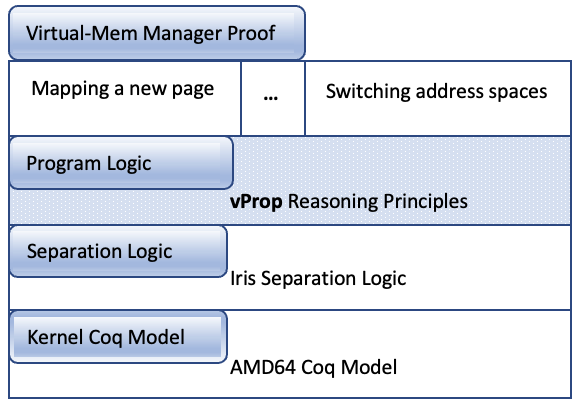
\includegraphics[width=0.5\columnwidth]{architecture.png}
%  \caption{Layers of Implementation}
%  \todo[inline]{Colin says: I don't think this figure helps readers; it is too abstract}
%  \label{fig:architecture}
%\end{figure}

\begin{itemize}
\item We develop these ideas in the form of a logic for working with virtual-address-space-relative assertions,
      implemented as an embedded separation logic within the Iris~\cite{jung2018iris} separation logic.
      The result is a separation logic that lifts a number of major semantic restrictions present in the few
      prior logics tackling virtual address translation.
\item We prove the soundness of our \textsf{vProp} logic with respect to a RISC-like fragment of \textsf{AMD64} instructions.
\item We verify simplified versions of several critical virtual-memory-related pieces of OS functionality, 
      including software page table walks, mapping  pages, and the assembly code for switching address spaces. 
      The latter in particular goes beyond the capabilities of prior work, and reveals unexpected
	subtleties.
\end{itemize}

The logic we develop here covers core reasoning principles for reasoning about memory configurations and code
reliant upon or manipulating those memory configurations in the presence of in-memory page tables, the primary
memory protection mechanism across Intel/AMD's x86-64 processors, ARM's application class processors including
aarch64 CPUs, POWER, RISC-V, and other architectures.
% One aspect of virtual memory management we do not address in this paper is updates to the translation lookaside
% buffer (TLB) present in most CPUs. Like CertiKOS~\cite{?}, seL4~\cite{sel4tocs}, and most other OS verification
% efforts we currently trust insertion of TLB flush operations, whose locations are critical but also few and
% well-known (after unmapping memory, or changing address spaces). Tackling correctness of TLB invalidation
% rigorously is an additional challenging project unto itself~\cite{...} with similarities to but
% significant divergences from reasoning about weak memory models, which future work should combine
% with the present work.

%\section{Motivation}
\label{sec:motivation}

IGNORE THIS FILE, WILL DO IN INTRO

\section{Background}
\label{sec:background}
This section briefly recalls both fundamentals of page-table-based address translation in
general-puspose OS kernels, 
high-level background on separation logics and the \iris~\cite{jung2018iris} framework
we build on,
and some material on modal logic that informs our development.

\subsection{Machine Model}
\label{sec:backgroundonmachinemodel}

In typical system configurations, all memory addresses seen by programs running on modern computers are \emph{virtualized}: the address observed by a running
program generally will not correspond directly to the physical location in memory, and may not even correspond to a physical location that \emph{exists} 
in the machine. Instead, these \emph{virtual} addresses are translated to \emph{physical} addresses that correspond directly to locations in RAM. On most 
modern architectures, this translation is performed through cooperation of the hardware and OS kernel: while executing an instruction that dereferences a 
(virtual) address, the CPU's \emph{memory management unit} (\textsc{MMU}) hardware performs \emph{address translation},
resulting in a physical address used to access the cache\footnote{Technically, for performance reasons most caches are indexed with parts of the virtual 
address, but tagged with the physical data addresses, so cache lookups and address translations can proceed in parallel.} and/or memory-bus.

\begin{figure}
%    \begin{framed}
%\column{.59\textwidth}    
\begin{subfigure}



\tikzset{every picture/.style={line width=0.75pt}} %set default line width to 0.75pt        

\begin{tikzpicture}[x=0.75pt,y=0.75pt,yscale=-0.5,xscale=0.5]
%uncomment if require: \path (0,430); %set diagram left start at 0, and has height of 430

%Shape: Rectangle [id:dp9406932326447903] 
\draw   (33,141) -- (123,141) -- (123,292) -- (33,292) -- cycle ;
%Shape: Rectangle [id:dp7682116051394419] 
\draw   (166,141) -- (256,141) -- (256,292) -- (166,292) -- cycle ;
%Shape: Rectangle [id:dp07376733516930423] 
\draw   (295,141) -- (385,141) -- (385,292) -- (295,292) -- cycle ;
%Shape: Rectangle [id:dp7106629147891306] 
\draw   (427,141) -- (517,141) -- (517,292) -- (427,292) -- cycle ;
%Shape: Rectangle [id:dp1342906826203598] 
\draw   (115,54) -- (185,54) -- (185,94) -- (115,94) -- cycle ;
%Shape: Rectangle [id:dp08072439007207399] 
\draw   (185,54) -- (255,54) -- (255,94) -- (185,94) -- cycle ;
%Shape: Rectangle [id:dp8282933603833216] 
\draw   (255,54) -- (325,54) -- (325,94) -- (255,94) -- cycle ;
%Shape: Rectangle [id:dp8416255090865326] 
\draw   (325,54) -- (395,54) -- (395,94) -- (325,94) -- cycle ;
%Shape: Rectangle [id:dp22911958218529804] 
\draw   (395,54) -- (465,54) -- (465,94) -- (395,94) -- cycle ;
%Shape: Rectangle [id:dp33732955213990756] 
\draw   (465,54) -- (535,54) -- (535,94) -- (465,94) -- cycle ;
%Curve Lines [id:da6688730321284677] 
\draw    (211.5,96) .. controls (-36.44,98.94) and (15.75,190.24) .. (30.17,213.65) ;
\draw [shift={(31,215)}, rotate = 238.24] [color={rgb, 255:red, 0; green, 0; blue, 0 }  ][line width=0.75]    (10.93,-3.29) .. controls (6.95,-1.4) and (3.31,-0.3) .. (0,0) .. controls (3.31,0.3) and (6.95,1.4) .. (10.93,3.29)   ;
%Shape: Rectangle [id:dp6044747978986409] 
\draw   (33,191) -- (123,191) -- (123,231) -- (33,231) -- cycle ;
%Curve Lines [id:da8867562998134584] 
\draw    (289.5,95) .. controls (115.15,110.76) and (137.77,175.03) .. (163.33,197.98) ;
\draw [shift={(164.5,199)}, rotate = 220.24] [color={rgb, 255:red, 0; green, 0; blue, 0 }  ][line width=0.75]    (10.93,-3.29) .. controls (6.95,-1.4) and (3.31,-0.3) .. (0,0) .. controls (3.31,0.3) and (6.95,1.4) .. (10.93,3.29)   ;
%Shape: Rectangle [id:dp8861153167245819] 
\draw   (166,177) -- (256,177) -- (256,217) -- (166,217) -- cycle ;
%Shape: Rectangle [id:dp05979844200848894] 
\draw  [dash pattern={on 4.5pt off 4.5pt}] (295,156) -- (385,156) -- (385,196) -- (295,196) -- cycle ;
%Shape: Rectangle [id:dp17403733244247843] 
\draw   (427,212) -- (517,212) -- (517,252) -- (427,252) -- cycle ;
%Curve Lines [id:da20581124900573955] 
\draw [color={rgb, 255:red, 0; green, 0; blue, 0 }  ,draw opacity=1 ] [dash pattern={on 4.5pt off 4.5pt}]  (357,97) .. controls (262.92,110.72) and (272.56,148.45) .. (291.81,173.48) ;
\draw [shift={(293,175)}, rotate = 231.34] [color={rgb, 255:red, 0; green, 0; blue, 0 }  ,draw opacity=1 ][line width=0.75]    (10.93,-3.29) .. controls (6.95,-1.4) and (3.31,-0.3) .. (0,0) .. controls (3.31,0.3) and (6.95,1.4) .. (10.93,3.29)   ;
%Curve Lines [id:da07589611603635316] 
\draw    (425.5,95) .. controls (380.42,119.5) and (406.41,202.58) .. (422.53,224.72) ;
\draw [shift={(423.5,226)}, rotate = 231.34] [color={rgb, 255:red, 0; green, 0; blue, 0 }  ][line width=0.75]    (10.93,-3.29) .. controls (6.95,-1.4) and (3.31,-0.3) .. (0,0) .. controls (3.31,0.3) and (6.95,1.4) .. (10.93,3.29)   ;
%Curve Lines [id:da6852167546673456] 
\draw    (497.5,95) .. controls (564.48,91.06) and (565,230.71) .. (567.87,269.31) ;
\draw [shift={(568,271)}, rotate = 265.24] [color={rgb, 255:red, 0; green, 0; blue, 0 }  ][line width=0.75]    (10.93,-3.29) .. controls (6.95,-1.4) and (3.31,-0.3) .. (0,0) .. controls (3.31,0.3) and (6.95,1.4) .. (10.93,3.29)   ;
%Curve Lines [id:da017521077423665377] 
\draw    (39.5,359) .. controls (-12.71,369.84) and (17.07,323.43) .. (32.31,293.36) ;
\draw [shift={(33,292)}, rotate = 116.57] [color={rgb, 255:red, 0; green, 0; blue, 0 }  ][line width=0.75]    (10.93,-3.29) .. controls (6.95,-1.4) and (3.31,-0.3) .. (0,0) .. controls (3.31,0.3) and (6.95,1.4) .. (10.93,3.29)   ;
%Curve Lines [id:da6750042432035159] 
\draw    (122,215) .. controls (128.9,254.4) and (131.91,269.54) .. (159.71,289.1) ;
\draw [shift={(161,290)}, rotate = 214.59] [color={rgb, 255:red, 0; green, 0; blue, 0 }  ][line width=0.75]    (10.93,-3.29) .. controls (6.95,-1.4) and (3.31,-0.3) .. (0,0) .. controls (3.31,0.3) and (6.95,1.4) .. (10.93,3.29)   ;
%Curve Lines [id:da14788158682113428] 
\draw    (257,197) .. controls (258.95,236) and (277.06,270.25) .. (293.72,290.47) ;
\draw [shift={(295,292)}, rotate = 229.64] [color={rgb, 255:red, 0; green, 0; blue, 0 }  ][line width=0.75]    (10.93,-3.29) .. controls (6.95,-1.4) and (3.31,-0.3) .. (0,0) .. controls (3.31,0.3) and (6.95,1.4) .. (10.93,3.29)   ;
%Curve Lines [id:da3297977595767969] 
\draw    (386,177) .. controls (392.86,226) and (408.36,270.2) .. (425.92,290.77) ;
\draw [shift={(427,292)}, rotate = 228.01] [color={rgb, 255:red, 0; green, 0; blue, 0 }  ][line width=0.75]    (10.93,-3.29) .. controls (6.95,-1.4) and (3.31,-0.3) .. (0,0) .. controls (3.31,0.3) and (6.95,1.4) .. (10.93,3.29)   ;
%Curve Lines [id:da7710391961792686] 
\draw    (517,229) .. controls (524.76,253.25) and (540.05,269.03) .. (552.82,282.73) ;
\draw [shift={(554,284)}, rotate = 227.12] [color={rgb, 255:red, 0; green, 0; blue, 0 }  ][line width=0.75]    (10.93,-3.29) .. controls (6.95,-1.4) and (3.31,-0.3) .. (0,0) .. controls (3.31,0.3) and (6.95,1.4) .. (10.93,3.29)   ;
%Shape: Rectangle [id:dp1535611125971872] 
\draw   (514,336) -- (584,336) -- (584,376) -- (514,376) -- cycle ;
%Shape: Rectangle [id:dp05427947476226991] 
\draw   (95,338) -- (136.5,338) -- (136.5,378) -- (95,378) -- cycle ;
%Shape: Rectangle [id:dp10511138743752002] 
\draw   (136.5,338) -- (265.5,338) -- (265.5,378) -- (136.5,378) -- cycle ;
%Shape: Rectangle [id:dp8917680919534263] 
\draw   (265.5,338) -- (305,338) -- (305,378) -- (265.5,378) -- cycle ;
\draw   (558,284.5) .. controls (558,279.25) and (562.25,275) .. (567.5,275) .. controls (572.75,275) and (577,279.25) .. (577,284.5) .. controls (577,289.75) and (572.75,294) .. (567.5,294) .. controls (562.25,294) and (558,289.75) .. (558,284.5) -- cycle ; \draw   (558,284.5) -- (577,284.5) ; \draw   (567.5,275) -- (567.5,294) ;
%Curve Lines [id:da9312068388962929] 
\draw    (568,298) .. controls (584.66,309.76) and (586.91,318.64) .. (565.35,335.93) ;
\draw [shift={(564,337)}, rotate = 321.95] [color={rgb, 255:red, 0; green, 0; blue, 0 }  ][line width=0.75]    (10.93,-3.29) .. controls (6.95,-1.4) and (3.31,-0.3) .. (0,0) .. controls (3.31,0.3) and (6.95,1.4) .. (10.93,3.29)   ;

% Text Node
\draw (11,14) node [anchor=north west][inner sep=0.75pt]   [align=left] {{\scriptsize Virtual}};
% Text Node
\draw (570,395) node [anchor=north west][inner sep=0.75pt]   [align=left] {{\scriptsize Physical}};
% Text Node
\draw (104,28) node [anchor=north west][inner sep=0.75pt]   [align=left] {{\scriptsize 63}};
% Text Node
\draw (175,28) node [anchor=north west][inner sep=0.75pt]   [align=left] {{\scriptsize 48}};
% Text Node
\draw (245,28) node [anchor=north west][inner sep=0.75pt]   [align=left] {{\scriptsize 39}};
% Text Node
\draw (314,28) node [anchor=north west][inner sep=0.75pt]   [align=left] {{\scriptsize 30}};
% Text Node
\draw (385,28) node [anchor=north west][inner sep=0.75pt]   [align=left] {{\scriptsize 21}};
% Text Node
\draw (454,28) node [anchor=north west][inner sep=0.75pt]   [align=left] {{\scriptsize 12}};
% Text Node
\draw (523,28) node [anchor=north west][inner sep=0.75pt]   [align=left] {{\scriptsize 0}};
% Text Node
\draw (132,65) node [anchor=north west][inner sep=0.75pt]   [align=left] {{\scriptsize Sign}};
% Text Node
\draw (195,65) node [anchor=north west][inner sep=0.75pt]   [align=left] {{\scriptsize L4 Offset}};
% Text Node
\draw (264,65) node [anchor=north west][inner sep=0.75pt]   [align=left] {{\scriptsize L3 Offset}};
% Text Node
\draw (336,65) node [anchor=north west][inner sep=0.75pt]   [align=left] {{\scriptsize L2 Offset}};
% Text Node
\draw (406,65) node [anchor=north west][inner sep=0.75pt]   [align=left] {{\scriptsize L1 Offset}};
% Text Node
\draw (472,65) node [anchor=north west][inner sep=0.75pt]   [align=left] {{\scriptsize Page Offset}};
% Text Node
\draw (67,63) node [anchor=north west][inner sep=0.75pt]   [align=left] {{\scriptsize va}};
% Text Node
\draw (53,203) node [anchor=north west][inner sep=0.75pt]   [align=left] {{\scriptsize L4 Entry}};
% Text Node
\draw (185,189) node [anchor=north west][inner sep=0.75pt]   [align=left] {{\scriptsize L3 Entry}};
% Text Node
\draw (316,167) node [anchor=north west][inner sep=0.75pt]   [align=left] {{\scriptsize L2 Entry}};
% Text Node
\draw (449,223) node [anchor=north west][inner sep=0.75pt]   [align=left] {{\scriptsize L1 Entry}};
% Text Node
\draw (51,347) node [anchor=north west][inner sep=0.75pt]   [align=left] {{\scriptsize root}};
% Text Node
\draw (465,349) node [anchor=north west][inner sep=0.75pt]   [align=left] {{\scriptsize page}};
% Text Node
\draw (532,346) node [anchor=north west][inner sep=0.75pt]   [align=left] {{\scriptsize 4K Data}};
% Text Node
\draw (156,386) node [anchor=north west][inner sep=0.75pt]   [align=left] {{\scriptsize 51}};
% Text Node
\draw (226,386) node [anchor=north west][inner sep=0.75pt]   [align=left] {{\scriptsize 12}};
% Text Node
\draw (145,350) node [anchor=north west][inner sep=0.75pt]   [align=left] {{\scriptsize Base Addr}};


\end{tikzpicture}
          \caption{Accessing to the Page Referenced by L1 Entry}
        \label{fig:enter-label}
    \end{subfigure}
    \vfill
    \begin{multicols}{2}
%    \begin{figure}
\begin{lstlisting}[mathescape,escapeinside={(*}{*)}]
/*
@param entry: entry whose frame address is used to locate the a-level-lower entry in the page-tree
@return next: return a virtual pointer to the descendant tree
*/
pte_t *pte_get_next_table(pte_t *entry) {
  pte_t *next;
  /*Reading page table entry justified by virtual pte-pointsto*/
  if (!entry->present(*\label{line:read_entry_contentsC}*) (*\label{line:conditional_childrenC}*)) {
    /* Jump if the present bit is not zero; no need to allocate next level (* \label{line:check_entry_presentC} *)(* \label{line:mask_presentC} *)  (*\label{line:after_concluding_qfrac1C}*)*/
    /*Allocation path starts here (*\label{line:pass_addrof_nextC}*)(*\label{line:alloc_path_startC}*)*/
    pte_initialize(entry);(* \label{line:call_to_pte_initializeC} *)
    /*Entry value updates:*/
    entry->pfn = nextpaddr;
    entry->present = 1; (*\label{line:install_new_entryC}*)
    /*Now we know that entry is initialized, so we satisfy the condition to access children list */
  } (*\label{line:end_of_allocation_pathCB}*)
  /*Physical to virtual address mapping code segment starts here (*\label{line:finalpieceSB}*)*/
  uintptr_t next_phys_addr = PTE_PFN_TO_ADDR(entry->pfn)
  uintptr_t next_virt_addr = (uintptr_t) P2V(next_phys_addr); (*\label{line:p2vCB}*);
  next = (pte_t *) next_virt_addr;(*\label{line:finalpieceEB}*)
  return next;
}
\end{lstlisting}
\columnbreak
\begin{lstlisting}[mathescape,escapeinside={(*}{*)}]
pte_t *walkpgdir(pte_t *l4, void *va){ 
 pte_t *l4_entry = &l4[L4Offset(va)];
 pte_t *l3 = pte_nxt_table(l4_entry);
 pte_t *l3_entry = &l3[L3Offset(va)];
 pte_t *l2 = pte_nxt_table(l3_entry);
 pte_t *l2_entry = &l2[L2Offset(va)];  
 pte_t *l1 = pte_nxt_table(l2_entry);
 pte_t *l1_entry = &l1[L1Offset(va)];  
 return l1_entry
}
\end{lstlisting}
%          \caption{Walking page-table tree to locate L1 entry C-source code.}
%        \label{fig:enter-label}
 %   \end{figure}
\end{multicols}
%\end{framed}
    \vspace{-2.5em}
    \caption{x86-64 page table lookups.}
    \label{fig:pagetables}
    \vspace{-1em}
\end{figure}

On the x86-64 architecture, the \textsc{MMU}'s address translation uses a sparse hierarchical set of tables:
\emph{page tables} (referring to pages of memory). As Figure \ref{fig:pagetables} (based on Figure 5-17 of the 
AMD64 architecture manual~\cite{amd64_manual_vol2}\footnote{While x86 up through its 32-bit incarnation were due to Intel,
the x86-64 architecture as a 64-bit extension to x86 was originally due to AMD. As a result, it is sometimes also referred to as the \texttt{amd64} architecture.}) shows, 
address translation proceeds by repeatedly taking designated slices of the virtual address and indexing into a table.
The final lookup in the page tables gives the base physical address of a 4KB page of physical memory, to which the low-order
bits of the accessed virtual address are added to determine the actual physical address retrieved. 
On x86-64, standard configurations use 4 levels of page tables, labelled levels 4 through 1, with lookups in the level 
1 page table resulting in the actual page of physical memory holding the requested data, and the low-order 12 bits 
being used to index into this page.\footnote{Technically levels 1--3 have explicit historical names,
but for brevity and consistency, we simply number them, in keeping with the newer 5th level.
Our formalization
only deals with 4-level page tables, but is straightforwardly extensible to 5.}  
The translation process or algorithm is sometimes referred to as a \emph{page-table walk}. 
While Figure \ref{fig:pagetables} and most of our constants (how many levels, which virtual address bits index which
table levels) are specific to the x86-64 architecture, ARMv8 (a.k.a.\ 
\texttt{aarch64}), RISC-V, and PowerPC use similar hierarchical page tables for address translation.
RISC-V's \texttt{sv48} paging configuration~\cite[\S 4.5]{riscv-privileged} and AArch64's 4-level paging configuration
both split 64-bit virtual addresses at the same points to index into the respective tables, so most of what follows
is equally applicable to those architectures (the only difference is that page table entries place control bits of write access, etc.,
in different orders).

The entries of each table are 64 bits wide, but each points to a physical address aligned to 4KB (4096 byte) boundaries, which leaves 12 bits to spare to 
control a validity bit (called the \emph{present} bit), a read-write bit (which permits write access through the entry if and only if it is set), 
and a range of additional bits which can be used to control caching, write-through, and more. This paper will only consider the present bit (0).

The page tables are managed by the OS, typically by a \emph{virtual memory manager} (VMM).\footnote{Not to be confused with Virtual 
Machine Monitor. We focus on non-hypervisor scenarios, but hardware virtualization extensions for both 
x86-64 and ARM make use of an additional set of page tables translating what a \emph{guest} considers to be its 
(virtualized) physical memory to actual physical memory. Our contributions should offer value in this scenario as well.}
Typically each process has its own 
page table, which the OS registers with the CPU by storing the (page-aligned)
physical address of the root of the page table treethe start of the L4 table) in a 
specific register (\texttt{cr3}) as part of switching to a new process. 
Using different mappings, which map only disjoint portions of physical memory (with some exceptions in the next section) 
is how the OS ensures memory isolation between processes.

If an instruction is executed that accesses a virtual address that either has no mapping, or does not have a mapping permitting 
the kind of access that was performed (e.g., the instruction was a memory write, but the relevant address range was marked read-only in
the relevant page table entry), the hardware triggers a \emph{page fault}, transferring control to a \emph{page fault handler} registered 
with the hardware by the OS, allowing it to take corrective action.
If no mapping was supposed to exist, this is a program bug (e.g., dereferencing virtual address 0 / NULL)
and the faulting program should be terminated. But this can also be used for
specialized functionality and optimizations, such as \emph{paging} (saving room in physical RAM and deferring
unnecessary IO by only reading program code from disk when it is accessed, or even swapping memory that has not
recently been accessed to disk, to read back in when a page fault indicates access).

The key pieces of VMM functionality are
adding a new page mapping (whether the mapped page contains zeros, file data, or swap data), and removing an existing 
page mapping.
While this initially sounds like relatively modest functionality whose implementation may be complicated by hardware 
subtleties, correctness of even these basic operations are actually quite intrictate.
Notably, updates to the page tables are performed as writes to memory --- \emph{which are themselves subject to address translation},
and finding the correct page table to update requires converting between physical and virtual addresses.
In the case of changing the mappings for the currently-active set of page tables, 
\emph{the OS kernel is modifying the tables involved in its
own access of the tables}.

Virtual memory concerns propagate to the OS scheduler, which deals with multiple 
address spaces, so must keep track of which virtual addresses are valid (and in what way) in which address spaces. 
Some virtual addresses are valid in only a single address space (e.g., a code address for a particular usermode 
process), while others are valid in all address spaces (e.g., kernel data structure pointers). 
The VMM must maintain some of these assumptions on behalf of the rest of the kernel, for example by guaranteeing that 
a certain range of virtual addresses (corresponding to the kernel's code and data) are valid in every address space.

\paragraph{Out of Scope: Translation Lookaside Buffers (TLBs)}
CPUs with MMUs typically have an additional \emph{translation lookaside buffer}
(TLB), to cache the (successful) results of page table walks, rather than transforming every virtual
memory access into 5 physical accesses. 
Any time a virtual address that was accessible becomes inaccessible (or has downgraded permissions),
the TLB (or at least entries in affected virtual address ranges) should be flushed.
In most kernels, this occurs in only a few well-known places, which is why existing verified kernels
\textsc{seL4}~\cite{Klein2009seL4,seL4TOCS} and \textsc{CertiKOS}~\cite{gu15,gu2016certikos} currently
trust that TLB flushes are handled correctly rather than actually modeling TLB hardware and verifying.
Eventual verification of TLB handling is a worthwhile long-term goal, but it is a challenging pursuit in its
own right. Based on others' early progress on verifying TLB operations in isolation~\cite{syeda2020formal}, we expect
it to be possible to combine this paper's insights with that support. 
Section \ref{sec:relwork} elaborates briefly on the challenges involved.
Even without TLB modeling,
our logic already enables verification of virtual memory management functionality that prior verified kernel work
either trusts completely (\textsc{seL4}, \textsc{CertiKOS}) or is incapable of reasoning about.
% Appendix \ref{apdx:tlb} gives more details on the challenges involved for the interested reader.
\looseness=-1

% \subsection{Virtual Memory Managers}
% \label{sec:backgroundonvmm}
% Most OS kernels have a component called a \emph{Virtual Memory Manager} (VMM)
% which is responsible for setting up page table mappings and for taking action when a page fault occurs. Often, a page 
% fault indicates a bug in a program --- for example, a null pointer dereference crashes a program not because the hardware
%  designates it an error, but because most OSes refuse to map the first 4K worth of virtual addresses, so dereferencing 
% \texttt{NULL} results in a page fault. In such cases, the OS will terminate the program.

% In other cases the OS uses page faults to implement specialized functionality and optimizations. A key example of this is 
% (confusingly) called \emph{paging}: saving room in physical RAM and avoiding unnecessary IO 
% by waiting until memory addresses for code are accessed 
% before copying them to RAM (in particular, saving process startup time); 
% or copying memory that has not recently been accessed to disk 
% (i.e., in a \emph{swap} file or partition) and marking those page table entries invalid so a future page fault will give 
% the OS the chance to copy the relevant data back into memory when the program tries to access it again.


% \todo[inline]{Colin says: we should chat about the paragraph below. We don't want to advertise too many
% challenges of VMM verification that we don't actually solve (or rather, we'd push them to the and of the paper
% as future work). But some of these I think we could split the difference with, for example by defining
% a variant of virtual-pointsto that allowed virtual address aliasing, but not actually verifying any code examples
% with it (just showing it's compatible with our approach).
% }
% For one, virtual addresses may \emph{alias} when more than one is mapped to the same physical memory. 
% This can occur when a process requests it (e.g., via \texttt{mmap} or \texttt{shm\_open} on UNIX-style kernels). 
% It also occurs automatically in most general-purpose kernels: while for normal programs the OS uses the MMU to isolate 
% and abstract physical memory, the kernel's own functionality is often easier to implement if the kernel can directly 
% access memory given its physical address, for example when interacting with hardware devices. For this reason, most 
% kernels contain an \emph{identity map} of all physical memory in a machine. 
% \todo[inline]{We should try defining an identity map on a whiteboard and see what breaks. If it's feasible we should
% tweak and get a definition in the paper. If not, we should cut the identity map discussion.}
% In some cases this is a literal identity map, 
% where for every virtual address $p$, interpreting $p$ as a virtual address instead will map back to $p$ as a physical 
% address. In other cases there is an offset involved, where to access physical address $p$ the kernel can access virtual
%  address $p+\mathit{offset}$. This identity map saves the kernel the performance cost of having to continually add and
%  remove transient mappings simply to briefly access a specific physical memory region. But this coexists with additional
%  virtual addresses (those used by most kernel code and data structures), in a form of virtual address aliasing. Note 
% that virtual address aliasing is both prevalent in general-purpose kernels, and violates the core assumption of most 
% memory models assumed by verified compilers like CompCert, which assume no virtual address aliasing.

% \todo[inline]{Colin says: Again, let's chat about the next paragraph. This might be another where we can
% split the difference on extension by defining something and proving a $\ast-\ast$ kind of result for sharing
% page table fragments, rather than actually proving any new code. I'm less sure about this one, though.
% }
% Another complicating factor is that portions of page tables can be shared, i.e., trees of page tables can overlap and
% become forests. 
% One common way this used to happen was for one subtree of page tables to map the kernel if linked in appropriately to 
% a higher-level page table, and then to reuse that kernel mapping portion in every process's page tables. This was mostly 
% phased out in the wake of Spectre, but remains relevant on correctly-implemented hardware.

\subsection{Separation Logic}
\label{sec:seplogic}
% \todo{Colin says: I added this b/c prior systems reviewers wanted more verification background...
% not sure how I feel about it}
Separation logic~\cite{reynolds02} is a descendant of classic Hoare logic~\cite{hoare69},
where in addition to pre- and postcondition assertions, assertions themselves pick up a
\emph{separating conjunction} operator $\ast$, such that an assertion $A\ast B$ means $A$ and $B$ are true
of disjoint pieces of state. This allows for local reasoning about updates, because it articulates
that updates to the state backing $A$ do not affect the truth of $B$. This is classically demonstrated
through the \emph{points-to} assertion: $l\mapsto v$ asserts that the memory cell at address $l$ holds value $v$:
knowing $x\mapsto 3\ast y\mapsto 4$ and writing through $x$ means information about $y$ is preserved:
$\{x\mapsto 3\ast P\}\;x\mathrel{:=}5\;\{x\mapsto 5 \ast P\}$ can be derived for any $P$.

We build on the \iris~\cite{jung2018iris} separation logic framework,
an abstract separation logic embedded in Rocq, which is useful for both metatheoretical work
and interactive correctness proofs using the logic. Given an operational
semantics structured a certain way (in our case, semantics for
a fragment of x86-64 assembly including address translation),
if a small number of ``glue'' lemmas are proven, \iris
provides a ready-made separation logic with a number of advanced features, including
higher-order ghost state and impredicative invariants, for no additional work.

We suppress many details of \iris assertions for brevity, but briefly note
a few recurring details used heavily in \iris but not necessarily in traditional
separation logics.
Because \iris is an embedded framework in \rocq, proofs in \iris-derived
logics (including ours) often encapsulate raw \rocq assertions: $\ulcorner P \urcorner$ is an embedding
of the \rocq assertion $P$ into an \iris assertion (used for things like equality and other
general pure logical assertions), similar to prior \rocq-embedded program logics~\cite{Chlipala2013Bedrock}. Newly-defined \iris assertions are in fact
\rocq terms of a particular type, rather than being drawn from a fixed vocabulary.
We introduce other details as they arise.

\iris includes two forms of implication. The magic wand operator $\wand$ is an affine implication:
$A\wand B$ describes a resource which, if combined with a resource satisfying $A$, will satisfy $B$.
Notably, this implication involves no changes to ghost state. \iris, building on the Views framework~\cite{Dinsdale-Young2013Views},
also includes a \emph{view shift} operator $\vs$ which models updates to ghost state: $A \vs B$
means resources satisfying $A$ may be transformed into resources satisfying $B$, intuitively by updating only ghost state.\footnote{\iris
experts may note that this is \emph{technically} mildly misleading given how \iris's update modalities and weakest precondition
are defined, but
this is adequate intuition for non-experts in \iris to follow their use.
}
\looseness=-1

% Of particular interest to us, \iris's machinery is largely agnostic to the particular choice of
% \emph{resource algebra}\footnote{A modern descendant of the venerable partial commutative monoid used
% to abstractly model earlier separation logics~\cite{calcagno2007local}, 
% with additions to support the step-indexing required to solve the recursive domain equations
% that arise with higher-order ghost state and impredicativity~\cite{birkedal2011step,hobor2010theory}.
% }
% used to give algebraic semantics to the connectives of the assertion language.
% This means we can drop in an alternative model that naturally supports working with respect to
% a locally-fixed context, like an address space.

% Also relevant is that \textsc{Iris} naturally decomposes the traditional Hoare triple $\{P\}\;C\;\{Q\}$
% into the precondition implying the weakest precondition of the program with respect to the postcondition ---
% $P \wand \textsf{wp}\;C\;\{v\ldotp Q\}$.\footnote{An idea with long history~\cite{pratt1976semantical}.}
% This is a natural fit for assembly-level verification, where the \emph{Hoare double}

An important limitation here is that to date, every separation logic
has assumed that all pointer addresses are meant for use in a single address space, which avoided the
problem of tracking that certain points-to assertions are true only for certain address spaces, but not others.

\subsection{Modal Logic}
\label{sec:backgroundonmodallogic}
The problem of needing to keep track of things being true in some contexts and not in others is hardly unique to virtual 
memory management, and is the general insight behind most flavors of modal logic, which use
unary operators to express that a logical claim $P$ is \emph{contingently} true 
in certain other circumstances, such as in other times~\cite{pnueli1977temporal} or places~\cite{murphy2008type,gordon2019modal}.

%   A unifying concept across any modality is that they behave as applicative functors, 
% typically satisfying (directly, or as a derived law, depending on the modality):
% \[ (P\rightarrow Q) \rightarrow M(P) \rightarrow M(Q)\]
% %\todo[inline]{Ismail, I think this means we have pure intro, $\square P \mathrel{-\ast} [r](\square P)$ if I'm using the right symbol for pure assertions }
% %\todo[inline,color=red]{The above todo comment isn't quite right.
% %Purity is about being able to duplicate. You had defined another typeclass/property-of-assertions that meant it didn't
% %care what address space it was in (like physical pointstos). That's orthogonal to purity.
% %}
% Many modalities, so-called \emph{normal} modalities also possess introduction rules of the form $P\rightarrow M(P)$, 
% the classic example being that if $P$ is true, then $P$ is \emph{necessarily} true with the contingency picked up.%($\square P$).

Of particular interest for reasoning about virtual memory are modalities that permit \emph{naming} the alternate 
circumstances, prominently \emph{hybrid} modal logics~\cite{blackburn1995hybrid,areces2001hybrid}, which come equipped 
with assertions of the form $[\ell](P)$ indicating that $P$ is true in the specific alternate circumstance (Kripke world)
 named by the \emph{nominal} $\ell$. Note that a distinctive property of hybrid logics is that, rather than hiding
the points at which a modal assertion is evaluated inside the modality's definition, the choice of what world a modalized
assertion should be true in is chosen \emph{in the assertion itself}. This allows assertions to talk about not simply whether some other assertion
is true in some possible future or past world related in a fixed way to the current world, but to talk about \emph{arbitrary}
other worlds. This explicit naming of alternate worlds increases the power of modal logics~\cite{blackburn1995hybrid}, and is actually
necessary for completeness in classical separation logics~\cite{brotherston2014parametric}.
%   A key distinguishing feature of
% hybrid logic is that the logic itself does not fix the set of modalities, but is defined relative to any set of sensible worlds.

For our purposes, these are natural candidates to adapt for virtual memory management. We can reinterpret the notion of 
naming an alternate world slightly more loosely, and instead name \emph{address spaces} by the physical address of the 
page table root, since these structures are the physical representations of page tables. Thus in this paper we develop 
the notion that we can represent contingent truth of an assertion via $[r](P)$ indicating that $P$ holds in the address 
space rooted at physical address $r$. Because OS kernels create and destroy address spaces, it is sensible to use
a hybrid-style logic that is not specialized to a fixed set of modalities, but this introduces
some subtleties from the fact that the existence of certain modalities (address spaces) can change.

% The typical hybrid modality introduction rule, that $P$ and $\ell$ (indicating the current world is $\ell$) imply 
% $[\ell](P)$, has a natural analogue: knowing $P$ and that the current address space is $r$ (i.e., that $r$ is the 
% current \texttt{cr3} value) suggests a way to construct $[r](P)$. 
% We identify an assertion as \emph{contextual} if its validity depends on the choice of address space. Used outside an explicit
% modality, the truth of this assertion depends on the current \texttt{cr3} value. Used under an explicit address space
% modality, its truth depends on both the modality-chosen address space and associated physical resources.
% \begin{itemize}
%   \item as a \textit{contextual} fact if its validity depends on \texttt{cr3} when it is outside the modality (i.e. modal context), and made 
%   \texttt{cr3} independent as a part of custom-tailored modal logic for virtual-memory: a truth representing a virtual-memory addressing depends
%    \texttt{cr3} due to address-translation operation, is dependent on \texttt{cr3} in the ambient-logic (e.g. separation-logic),
%     and is made \textit{independent} of the facts related to \texttt{cr3} by being introduced into the modal context under the assumption that
%     it exhibits the knowledge on its validity with respect to \texttt{cr3} in the ambient logic.
%   \item as a \textit{pure} fact as long as it does not \textit{necessarily} depend on any fact related to \texttt{cr3}: a truth representing a raw physical memory addressing, unlike virtual-address translation, does not need the \textit{knowledge} of \texttt{cr3}, therefore it can be introduce into the modal context as a pure fact
% \end{itemize}

Interaction of hybrid modalities and substructural reasoning is relatively unexplored (see Section \ref{sec:relwork}).
% A relatively under-explored space of modal logics is the interaction of modal and substructural logics, 
% in particular hybrid-style modalities in substructural logics, which has seen only minimal exploration~\cite{dovsen1992modal,restall1993modalities,d1997grafting,kamide2002kripke,licata2017fibrational} and no prior 
% application. 
Our development atop \iris~\cite{jung2018iris} needs to explore some additional subtleties 
that arise where the modality itself may entail ownership of resources, 
as well as interactions between our hybrid-style 
modality and substructural rules.  
% For example, Iris contains a number of modalities that distribute over separating 
% conjunction, or for which resources can freely move into the modality 
% (e.g., $\blacktriangleright(P)\ast Q \wand \blacktriangleright(P\ast Q)$). In our setting some of these rules 
% apply while others do not. For example, 
% In our setting, an assertion that involves no modalities is interpreted as 
% holding in the current (active-on-the-CPU) address space, so clearly cannot move into arbitrary other address spaces,
% while address-space-relative assertions 
% --- unless guarded by another address space modality.
Some prior \iris-based work~\cite{dang2019rustbelt,dang2022compass} has constructed derived modalities in the style we propose, indexed
by thread IDs. However in that setting, the intepretation of those modalities was fully fixed ahead of time (to refer to essentially buffers in operationalized versions of C11
concurrency). In this setting, while our modalities will be indexed by page table roots, it is possible to modify the address translation for an address
space with root $r$ --- thus changing the interpretation of a modality, and even whether a modality is valid --- \emph{while assertions with that modality are active}.
%
%
%Work on modal logic extends back for decades with many widely-varied variations; we discuss here only the pieces most relevant to our work.
%Broadly speaking modal logics incorporate \emph{modal operators}, which take as arguments a proposition expected to be true in another time~\cite{pnueli1977temporal}, place~\cite{gordon2019modal}\todo{other cites}, or circumstance~\cite{hintikka1962knowledge,halpern1985guide}, and result in a proposition true in the \emph{current} time, place, or circumstance at which the truth of the use of the modal operator is being evaluated. Classic examples include modal necessity $\square P$ describing that $P$ is \emph{necessarily} true, $\mathsf{G}~P$ meaning $P$ is true \emph{globally} (i.e., forever from this time onwards), or $K_i(P)$ describing that a particular participant $i$ \emph{knows} that $P$ is true. The latter is an example of of \emph{multimodal} logic, where there is an indexed family of modalities (modal operators) parameterized by some dimension of interest (there, participants).
%A closely related variant of multimodal logic is \emph{dynamic logic}~\cite{pratt1976semantical}, a logic of weakest preconditions~\cite{dijkstra-75} which works with modalities of the form $[p](P)$, which states that \emph{in the current program state}, \emph{if} program $p$ is run then afterwards $P$ will hold (modulo non-termination).
%This same idea is used to encode Hoare triples in the Iris program logic~\cite{krebbers2017essence}, using the same encoding as in Pratt's original presentation, where a Hoare triple $\{P\}C\{Q\}$ is encoded as $P\rightarrow[C](Q)$. Unlike classic work on dynamic logic~\cite{harel2000dynamic}, Iris applies these ideas in a \emph{substructural} setting (separation logic) where distributivity laws over substructural connectives must be considered. For both the dynamic modality and the later modality $\blacktriangleright$ used for guarded recursive predicates, these modalities satisfy axioms of the form $M(P)\ast Q\vdash M(P\ast Q)$, but not the reverse.
%Iris is not the first combination of modal and substructural logic~\cite{dovsen1992modal,restall1993modalities,d1997grafting,kamide2002kripke,licata2017fibrational}, but is certainly the most heavily tested.
%A hallmark of a unary logical operator $M$ being a modality is if $M$ satisfies an property akin to $(\upvarphi\rightarrow\psi)\rightarrow M(\upvarphi)\rightarrow\psi$, which roughly states that modus ponens holds under the modality.\footnote{Afficionados of modal logic will note that this property is not quite Axiom K (which requires the initial implication to also hold under $M$), but follows from K and a necessitation rule $\upvarphi\rightarrow M(\upvarphi)$. Non-necessitive modalities typically satisfy the weaker property we call out above.}
%Another pillar of our work is hybrid logic, a branch of modal logic with \emph{names} (called \emph{nominals} for states in Kripke models~\cite{blackburn1995hybrid,goranko1996hierarchies,areces2001hybrid,gargov1993modal}, in contrast to the typical flavor of modality which refers to an \emph{unspecified} (in the assertion) set of alternative circumstances. 
%
%Our work draws on ideas from hybrid modal logics, applied in the context of Iris's higher-order separation logic~\cite{jung2018iris}. We define our modalities and prove their rules directly within Iris, so there is no model-theoretic novelty in our work. Instead, we show that targeted use of modalities combining the ideas of \emph{named resources} with the power of substructural reasoning enable clear specification of general reasoning principles for data structures. Along the way we take advantage of the fact that modalities need not be injections between the \emph{same} logics, but in fact the propositions that modal operators contextualize can come from \emph{other} logics; in our case we exploit the fact that Iris itself is parameterized by a choice of step-indexed~\cite{ahmed-appel-virga-02} \textsf{BI}-algebra~\cite{ohearn1999bunched} to allow convenient specifications in embedded data-structure-relative logics.

\definecolor{dkgreen}{rgb}{0,0.6,0}
\definecolor{ltblue}{rgb}{0,0.4,0.4}
\definecolor{dkviolet}{rgb}{0.3,0,0.5}

% lstlisting coq style (inspired from a file of Assia Mahboubi)
\lstdefinelanguage{Coq}{ 
    % Anything betweeen $ becomes LaTeX math mode
    mathescape=true,
    % Comments may or not include Latex commands
    texcl=false, 
    % Vernacular commands
    morekeywords=[1]{Section, Module, End, Require, Import, Export,
        Variable, Variables, Parameter, Parameters, Axiom, Hypothesis,
        Hypotheses, Notation, Local, Tactic, Reserved, Scope, Open, Close,
        Bind, Delimit, Definition, Let, Ltac, Fixpoint, CoFixpoint, Add,
        Morphism, Relation, Implicit, Arguments, Unset, Contextual,
        Strict, Prenex, Implicits, Inductive, CoInductive, Record,
        Structure, Canonical, Coercion, Context, Class, Global, Instance,
        Program, Infix, Theorem, Lemma, Corollary, Proposition, Fact,
        Remark, Example, Proof, Goal, Save, Qed, Defined, Hint, Resolve,
        Rewrite, View, Search, Show, Print, Printing, All, Eval, Check,
        Projections, inside, outside, Def},
    % Gallina
    morekeywords=[2]{forall, exists, exists2, fun, fix, cofix, struct,
        match, with, end, as, in, return, let, if, is, then, else, for, of,
        nosimpl, when},
    % Sorts
    morekeywords=[3]{Type, Prop, Set, true, false, option},
    % Various tactics, some are std Coq subsumed by ssr, for the manual purpose
    morekeywords=[4]{pose, set, move, case, elim, apply, clear, hnf,
        intro, intros, generalize, rename, pattern, after, destruct,
        induction, using, refine, inversion, injection, rewrite, congr,
        unlock, compute, ring, field, fourier, replace, fold, unfold,
        change, cutrewrite, simpl, have, suff, wlog, suffices, without,
        loss, nat_norm, assert, cut, trivial, revert, bool_congr, nat_congr,
        symmetry, transitivity, auto, split, left, right, autorewrite},
    % Terminators
    morekeywords=[5]{by, done, exact, reflexivity, tauto, romega, omega,
        assumption, solve, contradiction, discriminate},
    % Control
    morekeywords=[6]{do, last, first, try, idtac, repeat},
    % Comments delimiters, we do turn this off for the manual
    morecomment=[s]{(*}{*)},
    % Spaces are not displayed as a special character
    showstringspaces=false,
    % String delimiters
    morestring=[b]",
    morestring=[d],
    % Size of tabulations
    tabsize=3,
    % Enables ASCII chars 128 to 255
    extendedchars=false,
    % Case sensitivity
    sensitive=true,
    % Automatic breaking of long lines
    breaklines=false,
    % Default style fors listings
    basicstyle=\small,
    % Position of captions is bottom
    captionpos=b,
    % flexible columns
    columns=[l]flexible,
    % Style for (listings') identifiers
    identifierstyle={\ttfamily\color{black}},
    % Style for declaration keywords
    keywordstyle=[1]{\ttfamily\color{dkviolet}},
    % Style for gallina keywords
    keywordstyle=[2]{\ttfamily\color{dkgreen}},
    % Style for sorts keywords
    keywordstyle=[3]{\ttfamily\color{ltblue}},
    % Style for tactics keywords
    keywordstyle=[4]{\ttfamily\color{dkblue}},
    % Style for terminators keywords
    keywordstyle=[5]{\ttfamily\color{dkred}},
    %Style for iterators
    %keywordstyle=[6]{\ttfamily\color{dkpink}},
    % Style for strings
    stringstyle=\ttfamily,
    % Style for comments
    commentstyle={\ttfamily\color{dkgreen}},
    %moredelim=**[is][\ttfamily\color{red}]{/&}{&/},
    literate=
    {\\forall}{{\color{dkgreen}{$\forall\;$}}}1
    {\\exists}{{$\exists\;$}}1
    {<-}{{$\leftarrow\;$}}1
    {=>}{{$\Rightarrow\;$}}1
    {==}{{\code{==}\;}}1
    {==>}{{\code{==>}\;}}1
    %    {:>}{{\code{:>}\;}}1
    {->}{{$\rightarrow\;$}}1
    {<->}{{$\leftrightarrow\;$}}1
    {<==}{{$\leq\;$}}1
    {\#}{{$^\star$}}1 
    {\\o}{{$\circ\;$}}1 
    {\@}{{$\cdot$}}1 
    {\/\\}{{$\wedge\;$}}1
    {\\\/}{{$\vee\;$}}1
    {++}{{\code{++}}}1
    {~}{{\ }}1
    {\@\@}{{$@$}}1
    {\\mapsto}{{$\mapsto\;$}}1
    {\\hline}{{\rule{\linewidth}{0.5pt}}}1
    %
}[keywords,comments,strings]

\section{Machine State \& Syntax}
\label{sec:syntax}
To develop our core logical ideas, we instantiate \textsf{Iris} with a simple language for streams of instructions, 
and a logical machine model corresponding to execution of x86-64 assembly instructions with virtual memory enabled on the 
CPU.

\subsection{Registers and Memory}
Programs we demonstrate in this paper requires accessing two types of computer resource: registers and memory.
 A register identifier, $\reg$, is chosen from a fixed finite set of register identifiers, $\regset$. 
We use these identifiers to access the register values, $\regval \in \regvaltype$.
\begin{figure}[t]
\newcommand{\commentary}[1]{ & \text{\small\it #1} \\}
\[
  \begin{array}{r@{\;}c@{\;}l}
    \loc & \in & \Loc \\
    \reg & \in & \regset \\
    \regval & \in & \regvaltype \\
    \val & ::= & \vunit

\\
    \instrs & ::= &
    \begin{array}[t]{@{}l@{\hspace{10mm}}l@{}}
    \begin{array}[t]{@{}ll@{}}
      \iskip
                   \commentary{no-op}
      \iseq\instr\instrs
                   \commentary{sequencing}
      % \ising\instr
                   % \commentary{executing}             
    \end{array}
    %&
    %\begin{array}[t]{@{}ll@{}}
     % \ialloc\lval\allocsize
      %             \commentary{heap allocation}
    %\end{array}
    \end{array}
    \\

    \ectx & ::= &
      \hole \mid
      \iseq\ectx\instrs 
    \\
  \end{array}
\]
\caption{Syntax}
\Description{Syntax}
\label{fig:syntax}
\end{figure}
Unlike registers, we do not abstract the memory indices as a special type but instead, for the sake of clarity and ease of representation, we show differently masked machine words, $\loc \in \Loc$, with the subscripts showing the length of a 64-bit machine word after masking, e.g. $\kw{w}_{12}$ is a 12-bit resource which can be obtained after masking 52-bit of a 64-bit word.
This simple syntax in Figure \ref{fig:syntax} includes a simple syntax for values because our language is purely \textit{imperative}, i.e. an instruction does not return a value. Intentionally, we restrict any stream of instruction, $\instrs$, to eventually reduce to $\iskip$ instruction. Our syntax capture the no-op ``$\iskip$'' and the sequencing construct ``$\iseq{\instr}{\instrs}$'' in their standard forms.
\subsection{State}
\label{sec:state}
%\todo[inline]{I don't think we need or want to describe the operational semantics in detail in the submission. It adds a lot of formalization that doen'st necessarily contribute to reader understanding. We should describe the runtime \emph{state} $\sigma$ of memory and registers, since that is directly used in interpreting assertions. But the reduction rules will mostly add mental overhead here.}
%\todo[inline,color=red]{Colin says: On the contrary, we must describe assembly instructions in enough detail for readers
%who aren't already assembly programmers to decode our examples! We don't have to talk about details of the formalization
%of the semantics, but we do need to talk about basic instructions we cover, basic patterns (like destination on the left),
%and just a bit about how all memory accesses implement Figure \ref{fig:pagetables}'s semantics.}
We represent the machine state mainly as a finite map of registers to register values and a map of masked physical memory addresses to 64-bit physical memory values. Together with default \textsf{CPU} instantiation, we end up having our state with following pieces:
\begin{itemize}
\item A constant cpu initialized with default value: $\sigma.\mathcal{C}$
\item A register map: $\sigma.\mathcal{R}: \kw{greg} \rightarrow_{\textrm{fin}} \kw{regval} $
\item A memory map: $\sigma.\mathcal{M}: \Locft \rightharpoonup_{\textrm{fin}} (\Loctw \rightharpoonup_{\textrm{fin}} \Locsf )$
\end{itemize}
As one might have already anticipated from the syntax we introduce, we do not bind any value of an evaluated expression. All the indices and accessed values are treated as globally referenced. In align with this design choice, our expression is a stream of instructions, which is not evaluated to a value to be bound, but changes the machine state through the indices (e.g. $\kw{r}\in\kw{greg}$) -- to the global maps.
\subsection{Instructions}
\label{sec:instructions}
Page-table walk shown in Figure \ref{fig:pagetables} is realized with physical memory \texttt{load}s and \textsf{store}s for the entries in the page-tables which are simply modelled as lookup and updates to an instance of a memory map with 64 bit entries. In the address translation,
\begin{lstlisting}[language=Coq]
 Definition translate (m: $\sigma.\mathcal{M}$) (root: word 64) (w: word 64): address :=
      let plm4e := translate_top_level m root  w in
      let pdpte := translate_from_l4e m pml4e w in 
      let pde := translate_from_l3e m pdpte w in
      let pte: = translate_from_l2e m pde w in
      let addr := translate_from_l1e m pte w in
      concat (shift_dropn addr 3 three_lt64) low3.
    end.
\end{lstlisting}
we see translation physical memory $\mathsf{load}$ for each level of page-table-walk, which is basically a table lookup with
\begin{lstlisting}[language=Coq]
   Definition load (mem: $\sigma.\mathcal{M}$) (w: { w: word 64 | aligned w }):word 64 + MemFail :=
    match  $\sigma$.mem !! (pfn (proj1_sig w)) with
      | None => inl (zero 64)
      | Some (inl page) => inl (page (page_off (proj1_sig w)))
      | Some (inr fault) => inr fault
      end.
  Definition store (mem: $\sigma.\mathcal{M}$) (w: { w: word 64 | aligned w }) (v: word 64):mem64 * (unit + MemFail) :=
    match $\sigma$.mem !! (pfn (proj1_sig w)) mem with
      | None =>
        (($\sigma.\mathcal{M}$<[(pfn (proj1_sig w)) := (inl (fun off =>
           if (word_dec off (page_off (proj1_sig w))) then v else zero 64))]> mem), inl tt)
      | Some (inl page) => (* update page contents *)
        (($\sigma.\mathcal{M}$<[(pfn (proj1_sig w)) := (inl (fun off =>
           if (word_dec off (page_off (proj1_sig w))) then v else zero 64))]> mem), inl tt)
      | Some (inr fault) => (mem, inr fault)
    end.
  Program Definition pfn (w : word 64) := shift_dropn w 12 _.
  Program Definition page_off (w : word 64) := bottomn w 12 _.
\end{lstlisting}
with frame and offset masking applied on the physical address being loaded. As expected \textsf{store} would be the update on the memory map entry
\todo[inline,color=yellow]{Colin, could you mention that we simplified the maps here to get rid of MemFail?}
After defining the translation in terms of physical load and store action, now we can define our \lstinline|mov| instructions.


%
%\subsection{Machine State under Address Translation}
%\label{sec:selectedinstrsemantics}
%Althought we give the complete set of operational semantics rule in \sref{appendix:movops}, It is worth building the intuition on the the way some of these rules bahave in the context of address translation. In fact $\readlval\maddr{\storememstar\crval}\locsf$ is unfoled into multiple physical memory lookups for the final page address retrieval -- i.e. address translation traversal as shown in Figure \ref{fig:pagetables}:
%\begin{itemize}
%\item top-level-address translation: with the given root address (64-bit $\crval$) of the address space, performs the address translation, handling the first level (to get the PML4 entry) itself. The next level table address is computed with the fetched PML4 offset value which exhibits itself as 9-bit offset in $\kw{maddr}$. \mytodo{iso: put move}
%\item translating from PML4 entry: performs the second level of address translation, to retrieve starting at the PML4 table entry, and interprets the PML4 entry that references a Page-Directory-Pointer Table (PDPT). We obtain the PDPT offset which exhibits itself as 9 bit offset in $\kw{maddr}$ to obtain the address of the next level page directory table (PDT) \mytodo{iso: put move}
%\item translating from PD entry: performs the third level of address translation, to retrieve starting at the PDP table entry, and interprets a PDPTE that references a PD table. Likewise, we obtain the PD offset which exhibits itself as 9 bit offset in $\kw{maddr}$ to obtain the address of the next level page directory table (PT) \mytodo{iso:put move }
%\item translate from PT entry: performs final level of address translation, starting from the PT entry, with a given 12 bit page offset, we can compute the physical address referencing $\locsf$ \mytodo{ismo: put mov}
%\end{itemize}

\section{Program Logic for Location Virtualization}
\label{sec:logic}
In this section, we describe our high-level reasoning principles for location virtualization whose detailed justification is shown in \sref{sec:soundness}. The principles shown here are mainly shaped around understanding and expressing the fact related the virtual address space, most specifically virtualization and translation of memory locations .
\subsection{Points-To Assertions}
\label{sec:pointsto}

We present three main points-to relations as part of utilization of separation logic \ref{} as an ambient logic:
\begin{enumerate}
\item Physical address points-to, $\pfpointsto\locsf\locsf\qfrac\ppts$
\item Register points-to, $\pfpointsto\rg\rv\qfrac\rpts$
\item Virtual memory address points-to, $\pfpointsto\vaddr\locsf\qfrac\vpts$
\end{enumerate}
\paragraph{Register points-to} The assertion $\pfpointsto\rg\rv\rpts\qfrac$ ensures the ownership of the register $\rg$ naming the register value $\rv$. The fraction $\qfrac$ with value 1 asserts the unique ownership of the register mapping, and grants update permission on it, otherwise, any value $0 < \qfrac <1$ represents partial ownership granting readonly permission on the mapping.
\paragraph{Physical-Memory points-to} The our physical memory points-to relation ($\pfpointsto\locsf\locsf\qfrac\ppts$) exhibits nested-mappings due to masking applied on the indexing address ($\locsf$). The unfolded definition of the physical mapsto 
\begin{figure}[!ht]
\[
\begin{array}{cl}
\pfpointsto\locsf\locsf\qfrac\ppts \stackrel{def}{=} & \nfpointsto{\mask\locsf\tw}{\mask\locsf\ft}\locsf\qfrac\naddr
\end{array}
\]
\caption{Physical Points-to with Nested Masking}
  \label{fig:physicalpointsto}
\end{figure}
where we simply abstract the generation of hierarchical mapping of a physical address ($\locsf$) through the different masks of the address ($\locsf|^{12}$ and $\locsf|^{52}$) as nested map resources.
\paragraph{Virtual-Memory points-to} As we see in Figure \fref{fig:}, virtual address mapping is obtained via traversal of page table, i.e. indirection provided by physical memory lookups. As expected, we define the virtual-points to relation, ($\pfpointsto\vaddr\locsf\qfrac\vpts$), in terms of multiple physical memory mappings representing the indirection shown in Figure \fref{fig:}
\begin{figure*}
\[
\begin{array}{l}
  \ppointsto\vaddr\locsf\vpts \stackrel{def}{=} \lambda \tlf\Loc.\\
  \exists_{\tlfoff\Locn \;, \tltoff\Locn \;, \tltwoff\Locn \;,\tlooff\Locn \;, \tpgoff\Loctw \;, \tlt\Loc \;, \tltw\Loc \;, \tlo\Loc \tpg\Loc} \ldotp \\
  \ulcorner \textsf{aligned } \vaddr \urcorner \star 
   \ulcorner \vaddr = \locsx :: \lfoff :: \ltoff :: 
   \ltwoff :: \looff :: \pgoff \urcorner \star\\
  \pfpointsto{\lvlsum\crt\lfoff}{\lvlbor\lt}\qfracfotsss\ppts \star 
  \pfpointsto{\lvlsum\lt\ltoff}{\lvlbor\ltw}\qfracfotss\ppts \star \\
  \pfpointsto{\lvlsum\ltw\ltwoff}{\lvlbor\lo}\qfracfots\ppts \star 
  \pfpointsto{\lvlsum\lo\looff}{\lvlbor\pg}\qfracfot\ppts \star \\
  \ppointsto{\pageptstosum\pg\pgoff}\locsf\ppts 
\end{array}
\]
\caption{Virtual Points-to Relation}
\todo[inline]{These fractions aren't quite right (though I see you added the variance between levels), I can walk you through in our meeting tomorrow.}
  \label{fig:virtualpointsto}
\end{figure*}
\section{Considering Hoare Doubles in the Context of Switching Address-Space}
An important subtlety arises with supporting \lstinline|mov|s into \lstinline|%cr3|. Consider the hypothetical rule:
\begin{mathpar}
\inferrule[Broken]{ }{
  \{P \ast cr3=r_1 \ast r=r_2 \ast [r_2](Q)\}
  \texttt{mov}~\texttt{\%cr3},~r%\lstinline|mov %cr3, r| 
  \{[r_1](P) \ast cr3=r_2 \ast r = r_2 \ast Q\}
}
\end{mathpar}
This rule captures the intuitive change of address space in a Hoare triple, rather than double, form. The problem with this is that it interacts quite poorly with the traditional frame rule and the modal flavor of virtual points-to assertions:
\begin{mathpar}
  \inferrule*[right=Frame]{
    \inferrule*[right=Broken]{ }{
    \{\mathsf{emp} \ast cr3=r_1 \ast r=r_2 \ast [r_2](Q)\}
    \texttt{mov}~\texttt{\%cr3},~r%\lstinline|mov %cr3, r| 
    \{[r_1](\mathsf{emp}) \ast cr3=r_1 \ast r=r_2 \ast Q\}
    }
  }{
    \{a\mapsto_\mathsf{v} x \ast \mathsf{emp} \ast cr3=r_1 \ast r=r_2 \ast [r_2](Q)\}
    \texttt{mov}~\texttt{\%cr3},~r%\lstinline|mov %cr3, r| 
    \{a\mapsto_\mathsf{v} x \ast [r_1](\mathsf{emp}) \ast cr3=r_1 \ast r=r_2 \ast Q\}
  }
\end{mathpar}
Notice that both the precondition and postcondition assert that $a\mapsto_\mathsf{v} x$ in the current address space, but we have no basis for concluding that address translation is preserved by the change of address space. So this derivation clearly leads to an unsound conclusion. This suggestss that the traditional frame rule and the Hoare triple presentation of the change-of-address-space rule cannot soundly coexist in the same system.
The heart of the problem is that while updating \lstinline|cr3| is \emph{physically} local, it globally changes the interpretation of virtual addresses. So it is simply unsound to frame around \lstinline|cr3| updates.

Switching to Hoare doubles resolves this problem because an under-appreciated subtlety of Hoare doubles is that typically \emph{there is no frame rule}. Instead each verification essentially includes a local frame that it passes to the next instructions (think continuation-passing style), giving each overall rule a \emph{global} (rather than local) precondition. For most rules this is not that important, but it does permit rules that have global effects on their preconditions.

This is then how we justify our actual rule for \lstinline|cr3| updates:
\begin{mathpar}
\inferrule[ChangeAddressSpace]{
  \{[r_1](P) \ast cr3=r_2 \ast r = r_2 \ast Q\}\overline{is}
}{
  \{P \ast cr3=r_1 \ast r=r_2 \ast [r_2](Q)\}
  \texttt{mov}~\texttt{\%cr3},~r;\;\overline{is}
  %\lstinline|mov %cr3, r| 
}
\end{mathpar}
Because the precondition on this rule is global, we avoid issues with framing.

If we wanted to consider a frame rule that would work for this logic, we could consider:
\begin{mathpar}
  \inferrule[Cr3Frame]{
    \{P\ast cr3=v\}\;C\;\{ Q \ast cr3=v\}
  }{
    \{R\ast P\ast cr3=v\}\;C\;\{ R \ast Q \ast cr3=v\}
  }
\end{mathpar}
By demanding that \lstinline|cr3| be held constant (or rather, at least restored to its original value) we could frame almost traditionally. In particular, this rule would work with framing around calls that might lead to address space switches, such as calling blocking operations in the kernel.

Readers familiar with dynamic frames~\cite{parkinson2011relationship} might find it useful to notice that a different perspective on this matter is that virtual points-to assertions are self-stable \emph{except} for changes in \lstinline|cr3|, so framing would then naturally require other means of holding \lstinline|cr3| constant (or saving and restoring it).
Virtual points-to assertions could be made self-stable by also giving them partial ownership over \lstinline|cr3| assertions, but this would require explicitly plumbing that ownership from \emph{all} assertions back to any place an address space change might occur; this would seem to be a far graver loss of modularity than this extra quirk in framing discussions.

%\definecolor{dkgreen}{rgb}{0,0.6,0}
\definecolor{ltblue}{rgb}{0,0.4,0.4}
\definecolor{dkviolet}{rgb}{0.3,0,0.5}

% lstlisting coq style (inspired from a file of Assia Mahboubi)
\lstdefinelanguage{Coq}{ 
    % Anything betweeen $ becomes LaTeX math mode
    mathescape=true,
    % Comments may or not include Latex commands
    texcl=false, 
    % Vernacular commands
    morekeywords=[1]{Section, Module, End, Require, Import, Export,
        Variable, Variables, Parameter, Parameters, Axiom, Hypothesis,
        Hypotheses, Notation, Local, Tactic, Reserved, Scope, Open, Close,
        Bind, Delimit, Definition, Let, Ltac, Fixpoint, CoFixpoint, Add,
        Morphism, Relation, Implicit, Arguments, Unset, Contextual,
        Strict, Prenex, Implicits, Inductive, CoInductive, Record,
        Structure, Canonical, Coercion, Context, Class, Global, Instance,
        Program, Infix, Theorem, Lemma, Corollary, Proposition, Fact,
        Remark, Example, Proof, Goal, Save, Qed, Defined, Hint, Resolve,
        Rewrite, View, Search, Show, Print, Printing, All, Eval, Check,
        Projections, inside, outside, Def},
    % Gallina
    morekeywords=[2]{forall, exists, exists2, fun, fix, cofix, struct,
        match, with, end, as, in, return, let, if, is, then, else, for, of,
        nosimpl, when},
    % Sorts
    morekeywords=[3]{Type, Prop, Set, true, false, option},
    % Various tactics, some are std Coq subsumed by ssr, for the manual purpose
    morekeywords=[4]{pose, set, move, case, elim, apply, clear, hnf,
        intro, intros, generalize, rename, pattern, after, destruct,
        induction, using, refine, inversion, injection, rewrite, congr,
        unlock, compute, ring, field, fourier, replace, fold, unfold,
        change, cutrewrite, simpl, have, suff, wlog, suffices, without,
        loss, nat_norm, assert, cut, trivial, revert, bool_congr, nat_congr,
        symmetry, transitivity, auto, split, left, right, autorewrite},
    % Terminators
    morekeywords=[5]{by, done, exact, reflexivity, tauto, romega, omega,
        assumption, solve, contradiction, discriminate},
    % Control
    morekeywords=[6]{do, last, first, try, idtac, repeat},
    % Comments delimiters, we do turn this off for the manual
    morecomment=[s]{(*}{*)},
    % Spaces are not displayed as a special character
    showstringspaces=false,
    % String delimiters
    morestring=[b]",
    morestring=[d],
    % Size of tabulations
    tabsize=3,
    % Enables ASCII chars 128 to 255
    extendedchars=false,
    % Case sensitivity
    sensitive=true,
    % Automatic breaking of long lines
    breaklines=false,
    % Default style fors listings
    basicstyle=\small,
    % Position of captions is bottom
    captionpos=b,
    % flexible columns
    columns=[l]flexible,
    % Style for (listings') identifiers
    identifierstyle={\ttfamily\color{black}},
    % Style for declaration keywords
    keywordstyle=[1]{\ttfamily\color{dkviolet}},
    % Style for gallina keywords
    keywordstyle=[2]{\ttfamily\color{dkgreen}},
    % Style for sorts keywords
    keywordstyle=[3]{\ttfamily\color{ltblue}},
    % Style for tactics keywords
    keywordstyle=[4]{\ttfamily\color{dkblue}},
    % Style for terminators keywords
    keywordstyle=[5]{\ttfamily\color{dkred}},
    %Style for iterators
    %keywordstyle=[6]{\ttfamily\color{dkpink}},
    % Style for strings
    stringstyle=\ttfamily,
    % Style for comments
    commentstyle={\ttfamily\color{dkgreen}},
    %moredelim=**[is][\ttfamily\color{red}]{/&}{&/},
    literate=
    {\\forall}{{\color{dkgreen}{$\forall\;$}}}1
    {\\exists}{{$\exists\;$}}1
    {<-}{{$\leftarrow\;$}}1
    {=>}{{$\Rightarrow\;$}}1
    {==}{{\code{==}\;}}1
    {==>}{{\code{==>}\;}}1
    %    {:>}{{\code{:>}\;}}1
    {->}{{$\rightarrow\;$}}1
    {<->}{{$\leftrightarrow\;$}}1
    {<==}{{$\leq\;$}}1
    {\#}{{$^\star$}}1 
    {\\o}{{$\circ\;$}}1 
    {\@}{{$\cdot$}}1 
    {\/\\}{{$\wedge\;$}}1
    {\\\/}{{$\vee\;$}}1
    {++}{{\code{++}}}1
    {~}{{\ }}1
    {\@\@}{{$@$}}1
    {\\mapsto}{{$\mapsto\;$}}1
    {\\hline}{{\rule{\linewidth}{0.5pt}}}1
    %
}[keywords,comments,strings]

\section{Implementing Logical Machinery \& Soundness}
We build our program logic, as an instantiation of Iris~\cite{iris}, and construct our reasoning principles including the modal one on top of it. 
\mytodo{we should put some stuff here}
\subsection{Soundness}
\label{sec:soundness}
Our logic, operates on the machine state, which means we do not need to augment the machine state. The invarian that we pick, \textit{central invariant} ($\textsf{x64\_h}$), is just semantic interpretation of stores in the machine state, $\sigma.\mathcal{R}$ and $\sigma.\mathcal{M}$. This semantic interpratation ensures the correct lifting of mappings in the machine state to the assertions that the client of our logic uses, i.e. points-to assertions that are defined as the ownership of a fragment of the logical state.

We prefer to skip explaining the steps used in instantiation of Iris because it is an almost standard procedure, has already been explained for many other logic \ref{}, and we are concerned with the page-count limitation. However, it is worh noting that once you instantiate Iris for your language, it comes with the semantic definition for the weakest-precondition which we can refactor into Hoare-Doubles to specify our  selected \textsf{AMD64} instructions shown in Figure \ref{fig:wpdamd}, and show that these triples are sound.
\subsection{The Soundness Statement}
\label{def:soundness:statement}
The operational semantics of our simple lang just executes sequences of instructions in our x86-64 model. Therefore, our soundness argument is to show that any execution composed of instructions in our machine model (some of which are shown in Figure \sref{sec:semantics}) does not end-up in a invalid state.
\begin{figure*}
\small
\begin{mathpar}
\inferrule[Skip]{}{
  \triple\post\iskip\post
}

\inferrule[Seq]{
  \triple\pre{\instr_1}\midpoint \\
  \triple\midpoint{\instr_2}\post
}{
  \triple\pre{(\iseq{\instr_1}{\instr_2})}\post
}
\end{mathpar}
\caption{Structural Rules for Executing Instructions}
\Description{Reasoning Rules}
\label{fig:structural}
\end{figure*}

\begin{theorem}[Soundness of the Logic]
  \label{th:adequacy}
 Together with the assumptions on the initial state hold,
 the execution of the instruction~$\instrs$, beginning with this initial state, cannot result in a configuration where the execution is stuck.
\end{theorem}
which states that if the program~$\instr$, with the given \textsf{valid\_init} asserting a valid state initialization, satisfies a semantic Hoare
triple, then this program cannot crash: by a direct consequence of Iris's adequacy theorem~\cite[\S6.4]{iris}.

Moreover we need to show the validity of each rules in Figures \fref{fig:reasoning} and \fref{fig:laws}.
\begin{theorem}[Validity of the Reasoning Rules]
\label{th:validity}
  Each of the rules in Figures~\ref{fig:wpdamd}
  and~\ref{fig:structural} is valid.
\end{theorem}
Due to the space limits in this paper, we do not mention each proof for the rules in Figures \ref{fig:wpdamd} and \ref{fig:structural} within this section, but we provide mechanized proofs for all these in Coq as a part of our artifact submission.
However, we would like to give the definitions and constructions used in our proofs, and would like to give an outline of paper proof for \TirNameStyle{WriteToRegFromVirtMem} in Figure \ref{fig:wpdamd} within this section.

Together, Theorems~\ref{th:adequacy} and~\ref{th:validity} guarantee that, if
the Hoare triple $\textsf{valid\_init }\instrs\;\iTrue$ can be obtained by applying
the reasoning rules of our logic, then the program~$\instrs$ is safe.

\subsection{Logical Constructions}
\label{sec:invariant}
We already have the physical and logical stores and a simple invariant between them. Now, we can rely on the following Assumption \ref{assumption} from Iris to utilize its logical constructions.
% The predicate gen_heap_interp.
\newcommand{\genheapinterp}[1]{\mathit{Heap}\;#1}
\newcommand{\genmemheapinterp}[1]{\mathit{MemHeap}\;#1}
% Our predicate pred (defined in ph.v), expanded.
\newcommand{\pred}[1]{\ownGhost\gammaPred{\authfull{(\mapone\predstore)}}}
% A notation for assigning fraction 1 to every element of \predstore.
\newcommand{\mapone}[1]{1.#1}
% The predicate mapsfrom_exact, expanded.
\newcommand{\mapsfromexact}[3]{
  \ownGhost\gammaPred{\authfrag{\singletonMap{#1}{(#2, #3)}}}
}
% A metavariable for a share.
\newcommand{\sh}{L'}
% The predicate mapsfrom, expanded.
\newcommand{\mapsfromdef}[3]{
  \exists\sh.\;
  \mapsfromexact{#1}{#2}{\sh} \star \pure{\sh \subseteq #3}
}

\begin{assumption}
\label{assumption}
Iris defines two pieces of ghost state
\begin{enumerate}
\item  defines a predicate $\textsf{to\_gen\_heap }\store.\mathcal{R}$
  that ties a store~$\store.\mathcal{R}$ to this ghost state,
  and defines the points-to assertion $\ppointsto\rg\rv\qfrac\rpts$
  in terms of this ghost state.
  This is visible in the paper~\cite[\S6.3.2]{iris}
  and in Iris's \texttt{gen\_heap} library~\cite{genheap}.
  %
  We re-use this machinery without change,
  so we do not repeat these definitions.
  We mention the predicate $\genheapinterp\!$
  in our own invariant (Definition~\ref{def:invariant}),
  where it is applied to the \logical store~$\store$.
\item unlike the register points-to relation obtained by direct interpretion of $\textsf{to\_gen\_heap }\store.\mathcal{R}$ using Iris, the existing \textsf{gen\_heap\_heap},
  does not directly helps introducing the ghost we define a new algebra (\textsf{gen\_mem\_UR}) for abstracting the nested maps due to different levels of masking in memory mappings and an interpretation for this algebra. 
\end{enumerate}
\end{assumption}

\begin{definition}[Ghost State - Memory with Nested Mappings]
We define our custom-tailored algebra 
\newcommand\fpfn{\rightarrow_{\textrm{fin}}}
\( \textsf{gen\_memUR} \stackrel{\triangle}{=}
  \authm(\;
  \Locft \;\fpfn\;
  (\Loctw \;\fpfn\;  (\textsc{Frac }, \mathord{+}) \times (\textsc{Agree } \Loc,\mathord{=}) )
  \)
  for our nested memory mapping abstracting two different machine word masking. To interpret this nested ghost map, i.e. obtain points-to assertions out of mappings in an ordinary \textsf{gmap}, we define \textsf{to\_gen\_mem}
  \begin{lstlisting}[language=Coq]
    Definition to_gen_mem : gmap L1 ( gmap L2 V) $\rightarrow$ gen_memUR L1 L2 V := fmap ($\lambda$ m . to_gen_heap m).
    Definition to_gen_heap : gmap L V $\rightarrow$ gen_heapUR L V :=  $\lambda$  v $\ldotp$ (1, to_agree (v :leibnizO V)).
  \end{lstlisting}
 throuh using \textsf{to\_gen\_heap} from previous Iris version. \todo[inline,color=red]{Ismail give exact version commit etc.}
\end{definition}

\begin{definition}[Ghost State - Register Mappings]
We allocate $\theta$ ghost cell which stores an
element of the monoid 
\newcommand\fpfn{\rightarrow_{\textrm{fin}}}
\(
  \authm(\;
    \regset \;\fpfn\;
    (\textsc{Frac}, \mathord{+})
    \times
    (\regvaltype, \mathord{=})
  \;)
\)
% \emph{authoritative camera}
\cite[\S6.3.3]{iris}.
\end{definition}

\begin{definition}[Central Invariant]
\label{def:invariant}
The central invariant of our logic is, due to lack of need for augmenting the machine state, simply the state interpretation: 
\[
\textsf{x64\_h}\;\store \triangleq
\def\arraystretch{1.2}
\begin{array}{l@{\quad\ast\quad}l@{\quad}l}
  \textsf{to\_gen\_heap} \;\store.\mathcal{R} & \textsf{to\_gen\_mem} \; \store.\mathcal{M}
\end{array}
\]
\end{definition}

As a last definition, we give the head step relation required for the Iris instantiation for our simple language in Figure \ref{} to sequence instructions. This relation allows lifting the program expression to enable the application of changes imposed by the operational semantics on the program state (for a certain cpu, a register map, and a selected memory for an address-space) when applied for an insturction (\textsf{i}).
\begin{lstlisting}[language=Coq]
Definition exec_step (i: instr) ($\sigma$:state) : option state :=
    exec_instr i $\sigma\mathcal{C}$ $\sigma.\mathcal{R}$ ((memToPhysMem $\sigma.\mathcal{M}$)  ($\sigma.\mathcal{R}$ !!  cr3)).
\end{lstlisting}
\todo[inline,color=yellow]{Colin, in case needed,not proven, could you simply say that we assume these map equalities or a paper proof etc.}. Again, due to the page limits, we can only give an outline of proof for a selected instruction (\TirNameStyle{WriteToRegFromVirtMem}) from our \textsf{AMD64} model. However, mechanized soundness proofs of other instructions can be found as a part of our submission artifact.

After obtaining ownership (points-to) predicates from application of state interpretation, now, we have well-enough definition for giving an outline for the proof of \TirNameStyle{WriteToRegFromVirtMem}.
 \begin{lemma}[\textsc{\TirNameStyle{WriteToRegFromVirtMem}}]
   \label{lemma:unlink}
\begin{align*}
\inferrule{
  \{P \ast r_d \mapsto_{r}  \textsf{v} \ast r_a \mapsto_{r} \{q\} \textsf{ vaddr} \ast \textsf{vaddr} \mapsto_{\textsf{v,rtv}} \textsf{v} \}_{\textsf{rtv}}\;\overline{is}
}{
  \{P \ast r_d \mapsto_{r}  \textsf{rvd} \ast r_a \mapsto_{r} \{q\} \textsf{ vaddr} \ast \textsf{vaddr} \mapsto_{\textsf{v,rtv}} \textsf{v} \}_{\textsf{rtv}}
  \textsf{mov}~\textsf{r}_d,~\textsf{r}_a;\;\overline{is}
}
\end{align*}
 \end{lemma}
 
 \begin{proof}
   Assuming the inference rule realized with \textsf{wpd\_def}, we expand the precondition with $\textsf{cr3} \mapsto_{\textsf{r}} \rtv$.
   Then we do two proofs, one for head reducibility of atomic step \textsf{mov\_reg64\_mem64}, the second one for the executing the expression and obtaining the new state. Steps taken in the first one are subset of the second one, so we outline the second portion of the proof, but in case of an interest in details of the proof, Coq artifact can be consulted.

   \begin{itemize}
   \item Step 1: we apply the head step relation and obtain the current valid state $\sigma1$ interpretation : $\textsf{x64\_h}\;\store$
   \item Step 2: we unfold the virtual-pointsto ($\vaddr \mapsto_{\textsf{v,rtv}} \textsf{v}$) definition, and for an existential physical page address $\paddr$, we exchange our fragmental toke ($\sumwalkabs\vaddr\qfrac\paddr$) to obtain physical table-pointsto ($\textsf{L}_{4}\_\textsf{L}_{1}\_\textsf{PointsTo}$ in Figure \ref{fig:strongvirtualpointsto}) relation
   \item Step 3: for each physical pointsto inside $\textsf{L}_{4}\_\textsf{L}_{1}\_\textsf{PointsTo}$, there exists a \textsf{load}, i.e. a concrete memory lookup
   \item Step 4: use these concrete lookups to traverse the page tables to obtain the value \textsf{v}
     \item Step 5: do the map update the $\sigma.\mathcal{R}$ for relevant register mapping ($r_d$) with the value \textsf{v} 
   \end{itemize}
   
   \end{proof}

%$\assert{\ulcorner \mathsf{aligned maddr} \urcorner \ast \mathsf{r14} \mapsto_{\textsf{r}} \textsf{r14v} \ast \mathsf{r13} \mapsto_{\textsf{r}} \textsf{maddr} \ast \mathsf{rdi} \mapsto_{\textsf{r}} \textsf{rdiv} \ast \mathsf{rax} \mapsto_{\textsf{r}} \textsf{raxv}}$
%$\assert{\ulcorner \ptablestore !! \textsf{maddr} = \textsf{None} \urcorner \ast \ownGhost\gammaPred{\authfull{\ptableabswalk\ptablestore}} \ast \textsf{Pf}} $
\definecolor{main-color}{rgb}{0.6627, 0.7176, 0.7764}
\definecolor{back-color}{rgb}{0.1686, 0.1686, 0.1686}
\definecolor{string-color}{rgb}{0.3333, 0.5254, 0.345}
\definecolor{key-color}{rgb}{0.8, 0.47, 0.196}

\lstdefinestyle{mystyle}
{
    language = C,
    basicstyle = {\footnotesize,\color{black}},
    backgroundcolor = {\color{white}},
    stringstyle = {\color{string-color}},
    keywordstyle = {\color{key-color}},
    keywordstyle = [2]{\color{lime}},
    keywordstyle = [3]{\color{yellow}},
    keywordstyle = [4]{\color{teal}},
    otherkeywords = {;,<<,>>,++},
    morekeywords = [2]{;},
    morekeywords = [3]{<<, >>},
    morekeywords = [4]{++},
    escapeinside={(*}{*)},
}
\newcommand{\sumwalkabsent}{
  \ownGhost\gammaPred{\authfrag{\singletonMap{\texttt{entry+KERNBASE}}{(\textsf{qfrac}, \textsf{entry})}}}
}


\newcommand{\ventry}{\texttt{entry + KERNBASE}}
\newcommand{\entry}{\texttt{entry}}
\newcommand{\qfraczero}{\textsf{qfrac}}
\newcommand{\true}{\textsf{true}}
\tikzstyle{boxedassert_border} = [sharp corners,line width=0.2pt]
\NewDocumentCommand \boxedassertpv {O{} m o}{%
	\tikz[baseline=(m.base)]{
		%	  \node[rectangle, draw,inner sep=0.8pt,anchor=base,#1] (m) {${#2}\mathstrut$};
		\node[rectangle,inner sep=1.5pt,outer sep=0.2pt,anchor=base] (m) {${\,#2\,}\mathstrut$};
		\draw[#1,boxedassert_border] ($(m.south west)$) rectangle ($(m.north east)$);
	}\IfNoValueF{#3}{^{\,#3}}%
}
\newcommand*{\knowInvpv}[2]{\boxedassertpv{#2}[#1]}
\newcommand*{\ownGhostpv}[2]{\boxedassertpv[dash dot]{#2}[#1]}

\newcommand{\sumpv}[3]{
  \ownGhostpv\gammaPred{\authfrag{\singletonMap{#1}{(#2, #3)}}}
}

\newcommand{\pvmapping}[1]{\mathcal{A}\textsf{PVMappings}(#1)}


\newcommand{\fpaddr}{\texttt{fpaddr}}
\newcommand{\specline}[1]{{\color{blue}\left\{#1\right\}}}
\newcommand{\sumapacesfull}[2]{
  \ownGhost\gammaPreds{\authfull{\singletonMap{#1}{#2}}}
}
\section{Experiments}
\label{sec:experiment}
%To both validate and demonstrate the value of the modal approach to reasoning about virtual memory management, 
% we study several
% We validate our logic by studying
% distillations of key VMM functionality.
% real concerns of virtual memory managers.
% Recall from Section \ref{sec:logic} that virtual points-to assertions work just like regular points-to assertions, by design.
In this section we verify several critical and challenging pieces of VMM code.
First, in several stages, we work up to mapping a new page in the current address space.
This requires a number of independently challenging substeps: dynamically traversing a page table to find
the appropriate L1 entry to update; inserting additional levels of the page table if necessary (updating
the VMM invariants along the way);
converting the physical addresses found in intermediate entries into the corresponding virtual addresses
that can be used for memory access;
installing the new mapping;
and collecting sufficient resources to form a virtual points-to assertion.
Of these, only the second-to-last step (installing the correct mapping into the
current address space) has previously been formally verified with respect to a machine model with address translation.
Second, we formally verify a switch into a new address space as part of a task switch,
the first such verification handling both old and new processes' assertions (in different address spaces) at the time of the switch.

%\begin{comment}
%\todo[inline]{Identity mappings are difficult, and our current approach won't quite work. Consider trying to have a virtual pointsto for an actual page table entry (i.e., that one could use to update a page table mapping), while also having a virtual pointsto for an address that entry mapped. With the current (let's call it v1) solution, we can't actually have both of those simultaneously!  That's because the PTE pointsto will assert full ownership of the physical memory cell holding the PTE as its data value, while the virtual pointsto for the data mapped by that entry will \emph{also} assert (fractional) ownership of all entries a page table walk would traverse.
%}
%\todo[inline,color=violet]{This doesn't seem to cause issues with the mapping/unmapping examples, only with changing intermediate page table pointers. The mapping example requires a virtual pointsto for the blank PTE, and once filled in that ownership can be immediately split to create the 512 new virtual pointsto assertions for the newly mapped page. Conversely, for unmapping we'd assume ownership of all the relevant virtual pointsto assertions for the page we're unmapping, at which point we can (with a bit of work) show that they all correspond to the same L1 PTE, and extract the 512 fractional shares of that entry from the pointsto assertions.  But changing intermediate page tables, as one would do for coallescing or splitting a superpage while preserving the virtual-to-physical mappings, couldn't be done without some really complicated separating implication tricks.}
%\todo[inline,color=green]{One possible approach to resolving this, which we came up with in our Tuesday meeting, is to recognize that the current (v1) virtual points-to is too strong, because it really doesn't care about \emph{owning} those fractional resources, it only cares that \emph{something} ensures the correct page table walk exists. Iris has a ghost map resource where authoritative ownership of an individual key-value pair can be handled as a resource.  (Colin was using this in the filesystem cache.)
%We can use that mechanism to separate the virtual-to-physical translation from the physical memory involved (Kolanski and Klein may have done something similar for different reasons): (fractional) virtual points-to assertions can be defined in terms of (fractional) ownership of these authoritative ghost map entry assertions, plus sharing an invariant that the current installed page table respects all entries of the mapping. Unmapping collects the authoritative map kvpairs from collecting the assertions, and then can remove them from the ghost map and update the page tables. Critically, physical ownership of the page tables then lives in the invariant on the current page table, so some virtual pointsto assertions can refer to memory in those page tables.
%This still works with the modality, since that invariant is also semantically a predicate on a page table root.
%Let's call this v2.
%}
%\end{comment}
\subsection{Traversing Live Page Tables}
\label{sec:traversing}
We build up to the main task of mapping a new page after traversing page tables in software.
The mapping operation of Figure \ref{fig:mapping_code} assumes an operation \textsf{walkpgdir} which must traverse the page tables
in order to locate the address of the L1 entry to update --- 
% possibly allocating tables for levels 3, 2, and 1 in the process,
% installing them into levels 4, 3, and 2, along the way.
possibly allocating new L3, L2, and L1 tables as necessary.
Traversing the page tables is itself challenging functionality to verify: loading the current table root from \lstinline|cr3| is straightforward
(a \lstinline|mov| instruction), however this produces the physical address of \lstinline|cr3|, not the virtual address the kernel code would use to access that memory.
This problem repeats at each level of the page table: assuming the code has \emph{somehow} read the appropriate L4 (or L3, or L2) entry, those entries again
yield physical addresses, not virtual.

\subsubsection{Loading Page-Table Address Value}
We will discuss access to the level 4 table later (Section \ref{wlkpgdir}). But for subsequent levels, the base address of level $n$ must be
fetched from the appropriate entry in the level $n+1$ table.
This is the role of \lstinline|pte_get_next_table| (Figures \ref{fig:calltopteinitialize} and \ref{fig:p2v}):
it is passed the virtual address of the page table entry in level $n+1$, and should return the \emph{virtual} 
address of the \emph{base} of the level $n$ table
indicated by that entry.
If the entry is empty (i.e., this is a sparse part of the page table representation),
the code also allocates a page for the level $n$ table, installs it in the level $n+1$ entry, and establishes appropriate invariants.
Figure \ref{fig:calltopteinitialize} presents the initial part of the function, which performs the allocation if necessary.
Figure \ref{fig:p2v} (discussed in Section \ref{sec:p2v}) deals with the cases where no allocation is necessary \emph{or} the allocation has already
been performed by the code in this figure.
\looseness=-1

Note that the specification does \emph{not} assume a specific page table level --- logical parameter \textsf{v} represents the level
of the entry passed as an argument, and this code
is used for all three level transitions when traversing page tables (4 to 3, 3 to 2, 2 to 1).
This comes into play with a subtlety of the specification of \lstinline|pte_get_next_table| that we will
revisit several times: \lstinline|pte_get_next_table|'s specification
assumes it is given a virtual \emph{vpte-pointsto}
(a virtual points-to exposing the underlying physical address instead of existentially quantifying it;
 see Section \ref{sec:mapnew}) granting access to the specified entry,
but its postcondition does not yield new virtual points-to assertions!
Instead it merely computes the base virtual address of the next table, and returns adequate capabilities (discussed in Section \ref{subsec:identitymappings})
for the \emph{caller} to construct a vpte-pointsto for any entry of the next table level (if this is not an L1 entry ---
the caller knows which level of the table this is for).
\looseness=-1

Within \textsf{get\_next\_table}, after a standard function prologue, the code 
loads the entry pointed to by the argument (logical variable \textsf{entry} in the proof outline).
This is a page table entry: a 64-bit word divided into bit-fields for
the physical address of the next table, and control bits like the valid bit, as discussed in 
Section \ref{sec:backgroundonmachinemodel}.



\ifPLDI
Line \ref{line:mask_present} checks % In the condensed figure, it's all on one line
\else
Lines \ref{line:mask_present}--\ref{line:check_entry_present} check
\fi
if the entry's ``present'' bit is set.
If it is zero, a new page must be allocated for the next level of the table --- which is done by the fall-through
from Line \ref{line:check_entry_present_jump}'s conditional jump. Otherwise the code jumps ahead to
the case for the next level already existing, which is discussed in Section \ref{sec:p2v} and Figure \ref{fig:p2v}.
First, we must discuss another refinement of the address space invariant, establishing
enough structure on the page tables themselves to allow the traversal.
The code for allocating a new level of the page table must establish this extended invariant.

%wshiftll (wshiftll (natToWord 64 entry) (WordImpl.concat (WordImpl.zero 56) (WordImpl.from_nat 8 12 ^& WordImpl.concat (WordImpl.zero 2) WO~1~1~1~1~1~1)) ^& constf)
%(WordImpl.concat (WordImpl.zero 56) (natToWord 8 12 ^& WordImpl.concat (WordImpl.zero 2) WO~1~1~1~1~1~1))
%
%wshiftll
 %      (wshiftll
%          ((((natToWord 64 entry ^& WordImpl.concat (WordImpl.zero 32) consta ^| WordImpl.concat (WordImpl.zero 32) (natToWord 32 2))
%             ^& WordImpl.concat (WordImpl.zero 32) constb ^| WordImpl.concat (WordImpl.zero 32) (natToWord 32 4)) ^& constd
%            ^| wshiftll
%                 (wshiftll (nextpaddr ^+ ^~ (natToWord 64 KERNBASE))
%                    (WordImpl.concat (WordImpl.zero 56) (WordImpl.from_nat 8 12 ^& WordImpl.concat (WordImpl.zero 2) WO~1~1~1~1~1~1))
%                  ^& constf)
%                 (WordImpl.concat (WordImpl.zero 56) (WordImpl.from_nat 8 12 ^& WordImpl.concat (WordImpl.zero 2) WO~1~1~1~1~1~1)))
%           ^& WordImpl.concat (WordImpl.zero 32) conste ^| wone 64)
%          (WordImpl.concat (WordImpl.zero 56) (WordImpl.from_nat 8 12 ^& WordImpl.concat (WordImpl.zero 2) WO~1~1~1~1~1~1)) ^& constf)
%       (WordImpl.concat (WordImpl.zero 56) (natToWord 8 12 ^& WordImpl.concat (WordImpl.zero 2) WO~1~1~1~1~1~1)) 
\begin{figure}%\footnotesize
\ifPLDI
\begin{lstlisting}[firstnumber=1, mathescape, language = C, style=mystyle]
/*
@param entry: entry whose frame address is used to locate the a-level-lower entry in the page-tree
*/
pte_t *pte_get_next_table(pte_t *entry) {
  pte_t *next;
  $\specline{\textsf{P} \ast \mathcal{I}\texttt{ASpace}_{\textsf{id}}(\theta,\Xi\setminus\{\textsf{entry}\},m) \ast \ghostmaptoken{\delta{}s}{\rtv}{\delta}  }_{\rtv}$
  $\specline{ \textsf{entry+KERNBASE} \mapsto_{\textsf{vpte,qfrac}} \textsf{entry entry\_val} \ast \ulcorner  \textsf{qfrac} = 1 \leftrightarrow \; \lnot(\textsf{entry\_present entry\_val})\urcorner}_{\rtv}$ (*\label{line:get_next_vpte_precondition}*)
  $\specline{\ulcorner\textsf{entry\_present(entry\_val)}\urcorner \wand \forall_{i\in\textsf{0..511}} \; \ghostmaptoken{\textsf{id}}{\textsf{table\_root(entry\_val.pfn) + i * 8}}{\textsf{v-1}} }_{\rtv} $ (*\label{line:conditional_children}*)
  /*reading page table entry Justified by virtual pte-pointsto*/
  if (!entry->present(*\label{line:read_entry_contents}*)) {/* Jump if the present bit is not zero; no need to allocate next level (* \label{line:check_entry_present} *)(* \label{line:mask_present} *) */
    /*Store the value of rbp minus 16 bytes (address of (*\textsf{next}*)) into rdi (*\label{line:pass_addrof_next}*)(*\label{line:alloc_path_start}*) */
    $\specline{ \textsf{entry+KERNBASE} \mapsto_{\textsf{vpte,qfrac}} \textsf{entry entry\_val} \ast \ulcorner  \textsf{qfrac} = 1 \land \lnot(\textsf{entry\_present entry\_val})  \urcorner }_{\rtv}$ (*\label{line:after_concluding_qfrac1}*)
    pte_initialize(entry);(* \label{line:call_to_pte_initialize} *)
    $\specline{ \ldots \ast \ulcorner  \textsf{qfrac} = 1 \land \lnot(\textsf{entry\_present entry\_val})  \urcorner \ast \ulcorner  \textsf{qfrac} = 1 \land \lnot(\textsf{entry\_present (pfn\_set (entry\_val nextpaddr))}  \urcorner   }_{\rtv}$
    $\specline{ \begin{array}{l}\textsf{entry\_present (pte\_initialized (pfn\_set(entryv nextpaddr)))} \wand  \\ \;\;\;\;\;\;\;\;\  \forall_{i\in \textsf{0 ... 511} } \ldotp  \ghostmaptoken{\textsf{id}}{((\textsf{table\_root (pte\_initialized (pfn\_set(entry\_val nextpaddr)))}) + \textsf{i * 8})}{\textsf{v-1}} \end{array}  }$ (*\label{line:page_of_caps}*)
    /*... entry value updates:*/
    entry->pfn = nextpaddr; entry->present = 1; (*\label{line:install_new_entry}*)
    /*... now we know that entry is initialized, so we satisfy the condition to access children list */
    $\specline{ \textsf{entry+KERNBASE} \mapsto_{\textsf{vpte,qfrac}}  \textsf{pte\_initialized(pfn\_set(entryv nextpaddr))} \ast \ulcorner  \textsf{qfrac} = 1 \land \lnot(\textsf{entry\_present entry\_val})  \urcorner }_{\rtv}$
    $\specline{\forall_{i\in \textsf{0 ... 511} } \ldotp  \ghostmaptoken{\textsf{id}}{((\textsf{table\_root (pte\_initialized (pfn\_set(entry\_val nextpaddr)))}) + \textsf{i * 8})}{\textsf{v-1}}  }$ (*\label{line:alloc_path_end}*)
  } (*\label{line:end_of_allocation_path}*)
  /*...  Code after conditional continued in Figure (*\ref{fig:p2v}*)*/
  $\specline{\textsf{P} \ast \mathcal{I}\texttt{ASpace}_{\textsf{id}}(\theta,\Xi\setminus \{ \mathsf{entry} \}),m) \ast \textsf{entry} \mapsto_{\textsf{id}} \textsf{\_} \ast \ghostmaptoken{\delta{}s}{\rtv}{\delta}  }_{\rtv}$
  $\specline{ \textsf{entry+KERNBASE} \mapsto_{\textsf{vpte,qfrac}} \textsf{(pte\_initialized (entry\_val.pfn))} \urcorner }_{\rtv}$
  $\specline{\forall_{i\in \textsf{0 ... 511} } \ldotp  \ghostmaptoken{\textsf{id}}{((\textsf{table\_root (pte\_initialized (entry\_val.pfn)))}) + \textsf{i * 8})}{\textsf{v-1}}  }$ (*\label{line:children}*)
  uintptr_t next_phys_addr = PTE_PFN_TO_ADDR(entry->pfn)
  uintptr_t next_virt_addr = (uintptr_t) P2V(next_phys_addr); (*\label{line:p2v}*);
  next = (pte_t *) next_virt_addr;
  return next;
}
\end{lstlisting}
\else
\begin{lstlisting}[mathescape, basicstyle=\footnotesize,escapeinside={(*}{*)}]
;;pte_t *pte_get_next_table(pte_t *entry) {
... ;; setting up the stack
;; pte_t *next;
$\specline{\textsf{P} \ast \mathcal{I}\texttt{ASpace}_{\textsf{id}}(\theta,\Xi\setminus\{\textsf{entry}\},m)  \ast \texttt{rbp-8} \mapsto_{\textsf{v}} \textsf{entry} \ast  \texttt{rbp-16} \mapsto_{\textsf{v}} \textsf{next} \ast \texttt{r8}  \mapsto_{\textsf{r}} \textsf{\_} \ast \texttt{rdi}  \mapsto_{\textsf{r}} \textsf{\_} \ast \ghostmaptoken{\delta{}s}{\rtv}{\delta}  }_{\rtv}$
$\specline{ \textsf{entry+KERNBASE} \mapsto_{\textsf{vpte,qfrac}} \textsf{entry entry\_val} \ast \ulcorner  \textsf{qfrac} = 1 \leftrightarrow \; \lnot(\textsf{entry\_present entry\_val})\urcorner}_{\rtv}$ (*\label{line:get_next_vpte_precondition}*)
$\specline{\ulcorner\textsf{entry\_present(entry\_val)}\urcorner \wand \forall_{i\in\textsf{0..511}} \; \ghostmaptoken{\textsf{id}}{\textsf{table\_root(entry\_val.pfn) + i * 8}}{\textsf{v-1}} }_{\rtv} $ (*\label{line:conditional_children}*)
mov    -0x8[rbp],rdi
$\specline{\textsf{P} \ast \mathcal{I}\texttt{ASpace}_{\textsf{id}}(\theta,\Xi\setminus\{entry\},m)   \ast \textsf{rbp-8} \mapsto_{\textsf{v}} \textsf{entry} \ast \texttt{r8}  \mapsto_{\textsf{r}} \textsf{\_}  \ast  \texttt{rbp-16} \mapsto_{\textsf{v}} \textsf{next} \ast \texttt{rdi}  \mapsto_{\textsf{r}} \textsf{entry} \ast \ghostmaptoken{\delta{}s}{\rtv}{\delta}  }_{\rtv}$
$\specline{ \textsf{entry+KERNBASE} \mapsto_{\textsf{vpte,qfrac}} \textsf{entry entry\_val} \ast \ulcorner  \textsf{qfrac} = 1 \leftrightarrow \; \lnot(\textsf{entry\_present entry\_val})\urcorner}_{\rtv}$
$\specline{\ulcorner\textsf{entry\_present(entry\_val)}\urcorner \wand \forall_{i\in\textsf{0..511}} \; \ghostmaptoken{\textsf{id}}{\textsf{table\_root(entry\_val.pfn) + i * 8}}{\textsf{v-1}} }_{\rtv} $
mov     rdi, r8
$\specline{\textsf{P} \ast \mathcal{I}\texttt{ASpace}_{\textsf{id}}(\theta,\Xi\setminus \{ \mathsf{entry} \},m)  \ast \textsf{rbp-8} \mapsto_{\textsf{v}} \textsf{entry} \ast \texttt{r8}  \mapsto_{\textsf{r}} \textsf{entry}  \ast  \texttt{rbp-16} \mapsto_{\textsf{v}} \textsf{next} \ast \texttt{rdi}  \mapsto_{\textsf{r}} \textsf{entry} \ast \ghostmaptoken{\delta{}s}{\rtv}{\delta}  }_{\rtv}$
$\specline{ \textsf{entry+KERNBASE} \mapsto_{\textsf{vpte,qfrac}} \textsf{entry entry\_val} \ast \ulcorner  \textsf{qfrac} = 1 \leftrightarrow \; \lnot(\textsf{entry\_present entry\_val})\urcorner}_{\rtv}$
$\specline{\ulcorner\textsf{entry\_present(entry\_val)}\urcorner \wand \forall_{i\in\textsf{0..511}} \; \ghostmaptoken{\textsf{id}}{\textsf{table\_root(entry\_val.pfn) + i * 8}}{\textsf{v-1}} }_{\rtv} $
mov    [r8],rdi (*\label{line:read_entry_contents}*)
$\specline{\textsf{P} \ast \mathcal{I}\texttt{ASpace}_{\textsf{id}}(\theta,\Xi\setminus \{ \mathsf{entry} \},m)  \ast \textsf{rbp-8} \mapsto_{\textsf{v}} \textsf{entry} \ast \texttt{r8}  \mapsto_{\textsf{r}} \textsf{entry}  \ast  \texttt{rbp-16} \mapsto_{\textsf{v}} \textsf{next} \ast \texttt{rdi}  \mapsto_{\textsf{r}} \textsf{entry\_val}  \ast \ghostmaptoken{\delta{}s}{\rtv}{\delta}  }_{\rtv}$
$\specline{ \textsf{entry+KERNBASE} \mapsto_{\textsf{vpte,qfrac}} \textsf{entry entry\_val} \ast \ulcorner  \textsf{qfrac} = 1 \leftrightarrow \; \lnot(\textsf{entry\_present entry\_val})  \urcorner }_{\rtv}$
$\specline{\ulcorner\textsf{entry\_present(entry\_val)}\urcorner \wand \forall_{i\in\textsf{0..511}} \; \ghostmaptoken{\textsf{id}}{\textsf{table\_root(entry\_val.pfn) + i * 8}}{\textsf{v-1}} }_{\rtv} $
and    0x1,rdi (* \label{line:mask_present} *)
mov    rdi,rax
cmp    0x0,rax ;;  if (!entry->present) {(* \label{line:check_entry_present} *)
jne    161 <pte_get_next_table+0xa1> (* \label{line:check_entry_present_jump} *) ;; Jump if the present bit is not zero
$\specline{\textsf{P} \ast \mathcal{I}\texttt{ASpace}_{\textsf{id}}(\theta,\Xi\setminus \{ \mathsf{entry} \},m)  \ast \textsf{rbp-8} \mapsto_{\textsf{v}} \textsf{entry} \ast \texttt{r8}  \mapsto_{\textsf{r}} \textsf{entry} \ast \texttt{rbp-16} \mapsto_{\textsf{v}} \textsf{next} \ast \texttt{rdi}  \mapsto_{\textsf{r}} \textsf{entry\_val \& 0x1} }_{\rtv}$
$\specline{  \textsf{entry} \mapsto_{\textsf{id}} \textsf{v} \ast \ghostmaptoken{\delta{}s}{\rtv}{\delta}  \ast \texttt{rax}  \mapsto_{\textsf{r}} \textsf{entry\_val \& 0x1} \ast \ulcorner\textsf{entry\_val \& 0x1}=\textsf{0x0}\urcorner}_{\rtv}$
$\specline{ \textsf{entry+KERNBASE} \mapsto_{\textsf{vpte,qfrac}} \textsf{entry entry\_val} \ast \ulcorner  \textsf{qfrac} = 1 \leftrightarrow  \lnot(\textsf{entry\_val \& 0x1}=\textsf{0x1})  \urcorner }_{\rtv}$ (*\label{line:before_concluding_qfrac1}*)
mov    rbp,rdi (*\label{line:alloc_path_start}*)
sub    0x10, rdi ;; Store the value of rbp minus 16 bytes (address of (*\textsf{next}*)) into rdi (*\label{line:pass_addrof_next}*)
$\specline{\textsf{P} \ast \mathcal{I}\texttt{ASpace}_{\textsf{id}}(\theta,\Xi\setminus \{ \mathsf{entry} \},m)  \ast \textsf{rbp-8} \mapsto_{\textsf{v}} \textsf{entry} \ast \texttt{r8}  \mapsto_{\textsf{r}} \textsf{entry} \ast \texttt{rbp-16} \mapsto_{\textsf{v}} \textsf{next} \ast \texttt{rdi}  \mapsto_{\textsf{r}} \textsf{rbp - 16} }_{\rtv}$
$\specline{  \textsf{entry} \mapsto_{\textsf{id}} \textsf{v} \ast \ghostmaptoken{\delta{}s}{\rtv}{\delta} }_{\rtv}$
$\specline{ \textsf{entry+KERNBASE} \mapsto_{\textsf{vpte,qfrac}} \textsf{entry entry\_val} \ast \ulcorner  \textsf{qfrac} = 1 \land \lnot(\textsf{entry\_present entry\_val})  \urcorner }_{\rtv}$ (*\label{line:after_concluding_qfrac1}*)
callq  70 <pte_initialize> ;;pte_initialize(entry);(* \label{line:call_to_pte_initialize} *)
$\specline{\textsf{P} \ast \mathcal{I}\texttt{ASpace}_{\textsf{id}}(\theta,\Xi\setminus \{ \mathsf{entry} \},m)  \ast \textsf{rbp-8} \mapsto_{\textsf{v}} \textsf{entry} \ast \texttt{r8}  \mapsto_{\textsf{r}} \textsf{entry}  }_{\rtv}$
$\specline{  \textsf{entry} \mapsto_{\textsf{id}} \textsf{v} \ast \ghostmaptoken{\delta{}s}{\rtv}{\delta} }_{\rtv}$
$\specline{ \textsf{entry+KERNBASE} \mapsto_{\textsf{vpte,qfrac}} \textsf{entry entry\_val} \ast \ulcorner  \textsf{qfrac} = 1 \land \lnot(\textsf{entry\_present entry\_val})  \urcorner }_{\rtv}$
$\specline{\ulcorner  \textsf{qfrac} = 1 \land \lnot(\textsf{entry\_present (pfn\_set (entry\_val nextpaddr))}  \urcorner   }_{\rtv}$
$\specline{ \texttt{rbp-16} \mapsto_{\textsf{v}} \textsf{pfn\_set(entry\_val nextpaddr)}   }_{\rtv}$
$\specline{ \begin{array}{l}\textsf{entry\_present (pte\_initialized (pfn\_set(entryv nextpaddr)))} \wand  \\ \;\;\;\;\;\;\;\;\  \forall_{i\in \textsf{0 ... 511} } \ldotp  \ghostmaptoken{\textsf{id}}{((\textsf{table\_root (pte\_initialized (pfn\_set(entry\_val nextpaddr)))}) + \textsf{i * 8})}{\textsf{v-1}} \end{array}  }$ (*\label{line:page_of_caps}*)
... ;;entry value updates: entry->pfn = nextpaddr; entry->present = 1; (*\label{line:install_new_entry}*)
... ;;now we know that entry is initialized, so we satisfy the condition to access children list
$\specline{\textsf{P} \ast \mathcal{I}\texttt{ASpace}_{\textsf{id}}(\theta,\Xi\setminus \{ \mathsf{entry} \},m)  \ast \textsf{rbp-8} \mapsto_{\textsf{v}} \textsf{entry} \ast \texttt{r8}  \mapsto_{\textsf{r}} \textsf{entry}  }_{\rtv}$
$\specline{  \textsf{entry} \mapsto_{\textsf{id}} \textsf{v} \ast \ghostmaptoken{\delta{}s}{\rtv}{\delta} }_{\rtv}$
$\specline{ \textsf{entry+KERNBASE} \mapsto_{\textsf{vpte,qfrac}}  \textsf{pte\_initialized(pfn\_set(entryv nextpaddr))} \ast \ulcorner  \textsf{qfrac} = 1 \land \lnot(\textsf{entry\_present entry\_val})  \urcorner }_{\rtv}$
$\specline{ \texttt{rbp-16} \mapsto_{\textsf{v}} \textsf{pte\_initialized(pfn\_set(entry\_val nextpaddr))}  \ast rax \mapsto_{r} \textsf{table\_root (pte\_initialized (pfn\_set(entry\_val nextpaddr)))}  }_{\rtv}$
$\specline{\forall_{i\in \textsf{0 ... 511} } \ldotp  \ghostmaptoken{\textsf{id}}{((\textsf{table\_root (pte\_initialized (pfn\_set(entry\_val nextpaddr)))}) + \textsf{i * 8})}{\textsf{v-1}}  }$ (*\label{line:alloc_path_end}*)
;;} (*\label{line:end_of_allocation_path}*)
... ;; Code after conditional continued in Figure (*\ref{fig:p2v}*)
\end{lstlisting}
\fi
% ;;uintptr_t next_virt_addr = (uintptr_t) P2V(next_phys_addr);
% movabs KERNBASE,rcx
% add    rcx,rax
% ...
% ;;next = (pte_t *) next_virt_addr;
% ;;clean up the stack and return next
% \end{lstlisting}
\vspace{-1em}
\caption{Ensuring \textsf{entry} points to a valid next table, allocating if necessary.}
\label{fig:calltopteinitialize}
\vspace{-1em}
\end{figure}

\subsubsection{Identity Mappings}
\label{subsec:identitymappings}
Kernels need to convert between physical and virtual addresses, in both directions.
Traversing the page tables in software is the simplest way to convert a virtual address to a physical address; this is the context we are working up to.
However, implementing this virtual-to-physical (V2P) translation in this way ironically requires physical-to-virtual (P2V) translation,
because the addresses stored in page table entries are physical, but memory accesses issued by the OS code use virtual addresses.
% There is no universal way to convert physical addresses to virtual --- doing so relies on the kernel maintaining careful invariants or
% additional data structures to enable P2V translation.
\looseness=-1

Because VMM operations are performance-critical for many workloads, most kernels 
maintain invariants that enable very fast P2V conversions (rather than adding another data structure).
Most kernels maintain an invariant on their page tables that the virtual address of any page used for a page table 
% lives at a virtual address whose value 
is \emph{a constant offset from the physical address} --- a practice sometimes referred to as \emph{identity mapping} 
(even though the physical-to-virtual translation
is typically not literally the identity function, but adding a non-zero constant offset).\footnote{Some kernels do this for all physical memory on the machine, simplifying interaction
with DMA devices.
On newer platforms like RISC-V, this sometimes truly is an identity mapping ---
x86-64 machines are forced into offsets by backwards compatibility with bootloaders that cannot access the full memory space of the
machine.
}

For this reason we extend the per-address-space invariant as in Figure \ref{fig:peraspaceinvariant_with_p2v_extension}, to also track which
addresses we can perform a P2V conversion on by a adding a constant offset.
$\Xi$ is another ghost map, from physical addresses to the level of the page table they represent (1--4).
\emph{Only} physical addresses in $\Xi$ can undergo P2V conversion. 
Section \ref{sec:p2v} describes the actual conversion,
but we describe the invariant here 
because adding new level 3/2/1 tables must maintain the invariant.

\begin{figure*}
\footnotesize
\[
\begin{array}{l}
  \mathcal{I}\textsf{ASpace}_{\textsf{id}}(\ptablestore,\Xi,m)\stackrel{\triangle}{=} \textsf{ASpace\_Lookup}_{\textsf{id}}(\ptablestore,\Xi,m) \ast \mathsf{GhostMap}(\mathsf{id},\Xi)\ast\\
  \left(\bigast{(\vaddr, \textsf{paddr})\in \ptablestore}{\exists\;(\textsf{l4e, l3e, l2e, l1e, paddr})\ldotp \textsf{L}_{4}\_\textsf{L}_{1}\_\textsf{PointsTo}(\vaddr\textsf{, l4e, l3e, l2e, l1e, paddr})}\right)\ast \\
  \bigast{(\paddr,\mathsf{level}) \in \Xi}{\exists\; (\textsf{qfrac, q, val,}\vaddr) \ldotp \ulcorner \vaddr = \paddr + \textsf{KERNBASE} \; \textsf{level} > 1\urcorner \ast  \underbrace{\fracghostmaptoken{\delta}{\vaddr}{\paddr}{\qfrac} }_\text{Ghost translation} \ast \underbrace{\paddr \mapsto_{\mathsf{p}}\{\textsf{qfrac}\}\; \vale}_\text{Physical location}} \ast\\
   \qquad\underbrace{ \ulcorner \textsf{qfrac} = 1 \leftrightarrow \; \lnot\textsf{entry\_present }(\vale) \urcorner}_\text{Entry validity}\ast 
    \underbrace{\left(\ulcorner\textsf{present\_L}(\vale,\mathsf{level})\urcorner \wand \forall_{\textsf{i}\in\textsf{0..511}} \ldotp \ghostmaptoken{\textsf{id}}{((\mathsf{entry\_page}\;\vale) + \textsf{i * 8})}{\textsf{level-1}}\right)}_{\text{Indexing into next level of tables}} \\
  \textsf{ where } \\
   \textsf{ASpace\_Lookup}_{\textsf{id}}(\ptablestore,\Xi,m) \stackrel{\triangle}{=} \lambda\textsf{ cr3val} \ldotp \; \exists \gammaPred \; \ldotp \ulcorner m \; !!\; \textsf{cr3val} = \textsf{Some } \gammaPred \urcorner \ast
   % \ownGhost\gammaPred{\authfull{\ptableabswalk\ptablestore}} \ast  \ownGhostpv\gammaPred{\authfull{\pvmapping\Xi}}
   \ptableabswalk{\delta,\ptablestore} \ast \pvmapping{\delta,\Xi}\\
  \textsf{present\_L}(\vale,\mathsf{level})\stackrel{\triangle}{=} \mathsf{entry\_present}(\vale)\land \mathsf{level} > 0
  
\end{array}
\]
\vspace{-1em}
\caption{Global Address-Space Invariant in Figure \ref{fig:peraspaceinvariant} extended with a ghost map bookkeeping identity mappings }
  \label{fig:peraspaceinvariant_with_p2v_extension}
\vspace{-1em}
\end{figure*}

For each $\paddr\mapsto \textsf{v} \in\Xi$, the invariant tracks a virtual points-to justifying that virtual address $\paddr+\textsf{KERNBASE}$ maps to physical address $\paddr$
(the ``Ghost translation'' in Figure \ref{fig:peraspaceinvariant_with_p2v_extension});
fractional ownership of the physical memory for that page table entry;
and for valid entries (with the present bit set) above L1, ghost map tokens for every entry in the table pointed to by the entry, which can be used
to repeat the process one level down. 
% (L1 entries point to data pages, whose physical memory ownership resides in some virtual points-to).
The assertion on Line \ref{line:conditional_children} of Figure \ref{fig:calltopteinitialize} comes from the invariant one level up; 
if the valid bit is set,
the code can return those child tokens without the conditional guard.
\looseness=-1

The fractional ownership of the entry's physical memory is subtle. Recall that $\textsf{L}_{4}\_\textsf{L}_{1}\_\textsf{PointsTo}$ retains some physical
ownership of each page table entry that is traversed (proportional to how many virtual addresses share the entry).
So in general the invariant cannot keep full permission to the memory in this part of the invariant, or it would overlap the page table walk for virtual points-to
assertions. But in the case where the entry is invalid, we may need to write to it (e.g., to install a reference to a next-level table, as we do in Figure \ref{fig:calltopteinitialize}),
which requires full permission. Fortunately, the entry can only be in use if its valid bit is set; if the valid bit is not set we know
that no virtual points-to entry in $\delta$/$\theta$ holds any partial ownership.
Thus we use the invariant portion annotated as ``Entry validity'' in Figure \ref{fig:peraspaceinvariant_with_p2v_extension} to capture this:
if the entry is invalid the invariant holds full ownership of the entry, so it can be updated; while if the entry is valid,
the invariant owns only a constant non-zero fragment sufficient to read the entry, but not modify it (which would invalidate some virtual points-to assertions):
\begin{equation*}
 \ulcorner \textsf{qfrac} = 1 \leftrightarrow \; \lnot\textsf{entry\_present }(\vale) \urcorner \tag{*}
\end{equation*}
Thus the fractional ownership of the physical location is enough for Line \ref{line:read_entry_contents} in Figure \ref{fig:calltopteinitialize} to access the entry, though in \lstinline|get_next_table|
the caller has pulled that piece of information out of the invariant and passed it for the entry at hand.
This removal appears explicitly in assertions,
as the argument to the invariant is $\Xi\setminus\{\mathsf{entry}\}$ (indexing by the set $\Xi$ allows us to borrow the physical resources
for a specific page table entry out of the invariant, and later put them back).
Line \ref{line:check_entry_present_jump}'s conditional then determines in the fall-through case that the bit is not set, which 
together with other facts entails $\textsf{qfrac} = 1$ at Line \ref{line:after_concluding_qfrac1},
and permits storing a new entry (in ellided code around Line \ref{line:install_new_entry}).
\looseness=-1

This seemingly-simple piece of code has a highly non-trivial correctness argument, which depends critically on detailed invariants on how access to page table
entries is shared between parts of the kernel. No prior work has engaged with this problem.

% Concretely speaking, going back to Line 15 in Figure \ref{fig:calltopteinitialize}, to read the value referenced by physical address \textsf{entry} while preserving the soundness of memory mappings, our extended invariant introduces the side condition (*)
% \begin{equation*}
%  \ulcorner \textsf{qfrac} = 1 \leftrightarrow \; \lnot\textsf{entry\_present }(\vale) \urcorner \tag{*}
% \end{equation*}
% assuring that looking the identity mapping for \textsf{entry} is safe under the subtle justification which equates the full ownership to the non/presence of the entry which can only be known when investigated in Line 21 in Figure \ref{fig:calltopteinitialize}.
\begin{comment}
 \begin{figure*}
   \footnotesize
   \[
 \begin{array}{l}
   \specline{\textsf{P} \ast \mathcal{I}\texttt{ASpace}_{\textsf{id}}(\theta,\Xi,m) \ast \textsf{rbp-8} \mapsto_{\textsf{v}} \textsf{entry} \ast \texttt{r8}  \mapsto_{\textsf{r}} \textsf{entry} \textsf{\_} \ast \ulcorner \Xi !! \textsf{entry} = \textsf{Some V} \urcorner  }_{\rtv}  \\
\sqsubseteq \\
   \specline{\textsf{P} \ast \mathcal{I}\texttt{ASpace}_{\textsf{id}}(\theta,\Xi\setminus \{ \mathsf{entry} \},m)  \ast \textsf{rbp-8} \mapsto_{\textsf{v}} \textsf{entry} \ast \texttt{r8}  \mapsto_{\textsf{r}} \textsf{entry}  \ast  \texttt{rbp-16} \mapsto_{\textsf{v}} \textsf{next} \ast \texttt{rdi}  \mapsto_{\textsf{r}} \textsf{entry} \ast \ghostmaptoken{\delta{}s}{\rtv}{\delta}  }_{\rtv} \\
\specline{ \textsf{entry+KERNBASE} \mapsto_{\textsf{vpte,qfrac}} \textsf{entry entry\_val} \ast \ulcorner  \textsf{qfrac} = 1 \leftrightarrow \; \lnot(\textsf{entry\_present entry\_val})\urcorner}_{\rtv} \\
\mathsf{mov} \;   [ \mathsf{r8} ],\mathsf{rdi}\\
 \specline{\textsf{P} \ast \mathcal{I}\texttt{ASpace}_{\textsf{id}}(\theta,\Xi\setminus \{ \mathsf{entry} \},m)  \ast \textsf{rbp-8} \mapsto_{\textsf{v}} \textsf{entry} \ast \texttt{r8}  \mapsto_{\textsf{r}} \textsf{entry}  \ast  \texttt{rbp-16} \mapsto_{\textsf{v}} \textsf{next} \ast \texttt{rdi}  \mapsto_{\textsf{r}} \textsf{entry} \ast \ghostmaptoken{\delta{}s}{\rtv}{\delta}  }_{\rtv} \\
\specline{ \textsf{entry+KERNBASE} \mapsto_{\textsf{vpte,qfrac}} \textsf{entry entry\_val} \ast \ulcorner  \textsf{qfrac} = 1 \leftrightarrow \; \lnot(\textsf{entry\_present entry\_val})\urcorner}_{\rtv} \\
 \end{array}
 \]
 \vspace{-1em}
\caption{Peel-out the resources needed for the virtual-pte pointsto relation for physical address \textsf{entry} to be accessed in Line 7 in Figure \ref{fig:calltopteinitialize}. }
  \label{fig:lookingupidpampping}
 \end{figure*}
\end{comment}


 \subsubsection{Installing a New Table}
 After obtaining the identity mapping for \textsf{entry}, we are able to load the \textsf{entry\_val} into \textsf{rdi}, and check the presence bit through
\ifPLDI
Line \ref{line:mask_present} % in condensed version, all on same line
\else
Lines \ref{line:mask_present}--\ref{line:check_entry_present} 
\fi
in Figure \ref{fig:calltopteinitialize}.
Accessing the presence bit and checking the value allows us to exploit the condition (*) that was just discussed when verifying the allocation
path (i.e., when the entry is invalid  and Lines \ref{line:alloc_path_start}--\ref{line:alloc_path_end} in Figure \ref{fig:calltopteinitialize}
must allocate the next level of tables).
This operation is subtle. To reiterate: the operation requires that the relevant table entry is readable, but the exact portion of ownership 
returned must be determined by inspecting the valid bit of the value in memory --- so full ownership is returned only for unused entries.
When the bit is not set, that entails full ownership of the entry's memory ($\textsf{qfrac} = 1$) and justifies writing to that memory.
Otherwise, the code jumps past the end of this listing, to the following code at the top of Figure \ref{fig:p2v} (which is also the
continuation of this code).

\begin{figure}\footnotesize
  \begin{lstlisting}[mathescape,escapeinside={(*}{*)}]
/*
@param entry: page entry whose frame is initialized with a new physical page 
*/
$\specline{\textsf{P} \ast \mathcal{I}\texttt{ASpace}_{\textsf{id}}(\theta,\Xi,m) \ast \lnot(\textsf{entry\_present entry\_val} }_{\rtv}$
$\specline{\textsf{entry+KERNBASE} \mapsto_{\textsf{vpte,1}} \textsf{entry entryv} \ast \ghostmaptoken{\textsf{id}}{(\mathsf{entry})}{\textsf{level}} }$
void pte_initialize(pte_t *entry) {
  /*allocate a full zeroed page for 512 8-byte entries(*\label{line:call_to_kalloc}*)*/
  pte_t *local = kalloc();
  entry->pfn = PTE_ADDR_TO_PFN((uintptr_t) local);
  $\specline{\textsf{P} \ast \mathcal{I}\texttt{ASpace}_{\textsf{id}}(\theta,\Xi,m) \ast \lnot(\textsf{entry\_present entry\_val}) }$
  $\specline{ \textsf{entry+KERNBASE} \mapsto_{\mathsf{vpte,1}} \mathsf{entry} \; \textsf{pfn\_set(entryv nextpaddr)}}$
  $\specline{\ghostmaptoken{\delta{}s}{\rtv}{\delta} \ast \begin{array}{l} \ulcorner\textsf{entry\_present (pte\_initialize(pfn\_set(entry\_val nextpaddr)),level)}\urcorner \wand \\  \;\;\;\;\;\;\; \forall_{i\in\textsf{0..511}} \; \textsf{table\_root (pte\_initialized (pfn\_set (entry\_val nextpaddr))) + i * 8} \mapsto_{\textsf{id}} \textsf{level-1}    \end{array}  }_{\rtv}$
  return;
}
\end{lstlisting}
\vspace{-1em}
\caption{Allocating a physical page }
\label{pteinitializespec}
\vspace{-1em}
\end{figure}

If the entry is not set, \textsf{pte\_initialize} (Line \ref{line:call_to_pte_initialize} in Figure \ref{fig:calltopteinitialize}) 
allocates a physical page (internally utilizing the only unverified (trusted) code in our case studies, the page-allocator's \textsf{kalloc},\footnote{
  This is an allocator for regions of pre-zeroed physical memory that is mapped, but not accessed by the allocator itself,
  as is typical for slab allocators~\cite{bonwick1994slab}.
  Its verification would be similar to verifying a usermode \textsf{malloc} verifications~\cite{Chlipala2013Bedrock,wickerson2010explicit},
  just with additional invariants on the memory pool.
} 
on Line \ref{line:call_to_kalloc} in Figure \ref{pteinitializespec}). 
Since we are using \textsf{pte\_initialize} for page-table address allocation, we must relate this newly
allocated physical address to the identity mapping map $\Xi$ --- 
see Line \ref{line:page_of_caps} in Figure \ref{fig:calltopteinitialize}, where
\texttt{kalloc}'s specification guarantees it has returned memory from a designated memory
pool that is already mapped
\ifPLDI
\else
\footnote{A reasonable reader might wonder where this pool
initially comes from, and how it might grow when needed. Typically an initial mapping subject to this identity mapping
constraint is set up prior to transition to 64-bit kernel code (notably,
a page table must exist \emph{before} virtual memory is enabled during boot, as part of enabling it is setting
a page table root).
Growing this pool later requires cooperation of physical memory range allocation and virtual memory range allocation,
typically by starting general virtual address allocation at the highest physical memory address plus the identity mapping offset.
This reserves the virtual addresses corresponding to all physical addresses plus the offset for later use in this pool,
as needed.
} 
\fi
and satisfies the offset invariants.
% \todo[inline,color=blue]{colin frontier.
% Stuck with line 31 onwards in Figure 7. rax holds nextpaddr, but I think that should be entrypfn, and 
% the explicit entrypfn id token assertion should go away, as its covered by the forall assertion.
% then the postcondition for pte-initialize should have a specific level now for the entries,
% like 0, which can be updated in the view shift on line 42.
% }
% Focusing on the specification of \textsf{pte\_initialize} separately in Figure \ref{fig:pteinitializespec}, 
% we right immediately realize that instead of seeing see a physical pointsto for the fresly page-table address 
% (e.g. $\mathsf{nextpaddr} \mapsto_{\mathsf{p}} \mathsf{w64\_0}$) deliberately in the post-conditoin in Lines 15-16,
%  we observe a full-ownership token representing the knowledge that a frame and all the entries indexed from this 
% frame are freshly allocated with full-ownership to be a part of the identity map, $\Xi$. 
The soundness argument of this specification relies on the fact that these freshly allocated resources are part 
of an entry construction that has not been completed yet: the presence bit is set 
(Line \ref{line:install_new_entry} in Figure \ref{fig:calltopteinitialize}) after these freshly allocated resources are incorporated to the 
entry construction via the page-frame portion of the PTE. In other words, the side condition, (*),
 formalizes that any access to the entry with these resources is \textit{invalid} (in the sense of not necessarily
having accompanying resources) until the entry is marked present (and thus the memory returned from \textsf{kalloc}
moves into the page table invariant.

\subsubsection{Physical-to-Virtual Conversion with \textsf{P2V}}
\label{sec:p2v}
Once we know the entry refers to a physical address in the identity mapping range ($\Xi$)
(via the branch at Line \ref{line:check_entry_present_jump}, or  by allocating and installing a new entry
as just discussed for Lines \ref{line:check_entry_present_jump}--\ref{line:end_of_allocation_path}), 
we can convert this frame address to a corresponding virtual address via the identity mappings
discussed in Section \ref{subsec:identitymappings} and Figure \ref{fig:peraspaceinvariant_with_p2v_extension}.
in the last lines of \lstinline|pte_get_next_table| shown in Figure \ref{fig:p2v} (the continuation of Figure \ref{fig:calltopteinitialize}).
This is a critical piece of the full page table walk verification.
In our small kernel (Line \ref{line:p2v} in Figure \ref{fig:p2v}), as in larger kernels, the C macro \texttt{P2V} common to many kernels
is actually just addition by the constant offset mentioned in Section \ref{subsec:identitymappings}.
But the correctness of this simple instruction is quite subtle.
%  and cannot be proven 
% without the extended invariant (Figure \ref{fig:peraspaceinvariant_with_p2v_extension})
% worked out Section \ref{subsec:identitymappings}.

%\begin{figure}\footnotesize
%  \begin{lstlisting}[mathescape,escapeinside={(*}{*)}]
%  /*... Continued from Figure (*\ref{fig:calltopteinitialize}*); assertions below specialized to non-allocating path for clarity */
%  $\specline{\textsf{P} \ast \mathcal{I}\texttt{ASpace}_{\textsf{id}}(\theta,\Xi\setminus \{ \mathsf{entry} \}),m)  \ast \textsf{rbp-8} \mapsto_{\textsf{v}} \textsf{entry} \ast \texttt{rcx}  \mapsto_{\textsf{r}} \textsf{\_}  \ast \textsf{entry} \mapsto_{\textsf{id}} \textsf{\_} \ast \ghostmaptoken{\delta{}s}{\rtv}{\delta}  }_{\rtv}$
%  $\specline{ \textsf{entry+KERNBASE} \mapsto_{\textsf{vpte,qfrac}} \textsf{(pte\_initialized (entry\_val.pfn))} \urcorner }_{\rtv}$
%  $\specline{ \texttt{rbp-16} \mapsto_{\textsf{v}} \textsf{(pte\_initialized (entry\_val.pfn)))} \ast \texttt{rax} \mapsto_{\textsf{r}} \textsf{ table\_root (pte\_initialize(entry\_val.pfn))} }_{\rtv}$
%  $\specline{\forall_{i\in \textsf{0 ... 511} } \ldotp  \ghostmaptoken{\textsf{id}}{((\textsf{table\_root (pte\_initialized (entry\_val.pfn)))}) + \textsf{i * 8})}{\textsf{v-1}}  }$ (*\label{line:children}*)
%  uintptr_t next_phys_addr = PTE_PFN_TO_ADDR(entry->pfn)
%  uintptr_t next_virt_addr = (uintptr_t) P2V(next_phys_addr); (*\label{line:p2v}*) 
%  /*... clean up the stack and return the rax value*/
%  return next
%}
%\end{lstlisting}
%\vspace{-1em}
%\caption{Converting a physical address of a PTE to a virtual address (w/o instruction pointer or flag updates).
% % Abreviating the other relevant resources (including the lower entries) peeled-out of the invariant as $\textsf{R}_{\textsf{children}}$
%\vspace{-1em}
%}
%\label{fig:p2v}
%\end{figure}
Figure \ref{fig:p2v} shows the verification of the end of \lstinline|pte_get_next_table| specialized to the case where 
where no allocation was necessary (i.e., the conditional on Line \ref{line:check_entry_present} of Figure \ref{fig:calltopteinitialize} was taken).
In this case, the true present bit allows access to the child tokens from Line \ref{line:conditional_children} of Figure \ref{fig:calltopteinitialize},
which is then refined to the assertion on Line \ref{line:children} of Figure \ref{fig:p2v}.
The code loads \lstinline|rcx| with the offset value \textsf{KERNBASE}, which gives us the value of the virtual address ($\textsf{entry}_{\textsf{pfn}}$ \textsf{+KERNBASE})
of the \emph{base} of the next level of the page table.
% \todo[inline]{the next sentence depends on having figure 10 updated to reflect the page-worth of tokens}
While we could now convert this address to a virtual points-to, this is not necessarily the correct thing to do.
The caller \lstinline|walkpgdir| (discussed next) uses \lstinline|pte_get_next_table| to retrieve just the base address,
because only the caller knows which entry in the subsequent table will be accessed (it depends on the corresponding bits from the virtual
address being translated). So instead we pass back the per-address-space invariant with the identity mapping resources for \lstinline|entry|
pulled out. The caller determines which entry in that table must actually
be accessed --- by selecting the appropriate index into the 512 ghost map tokens returned in the postcondition,
and using the ghost translation and physical location portions of the invariant to assemble a vpte-pointsto
that justifies the caller's subsequent access to a particular entry of the returned table.
% in the identity map ($\Xi\setminus\{entry\}$) of the kernel invariant.
% the logical update in Specification  Lines 5-10 to 10-14 for obtaining virtual-pointsto resource for the frame 
% ($\textsf{entry}_{\textsf{pfn}}$) by removing it from the ghost map ($\Xi\setminus\{entry\}\cup \{\textsf{entry}_{\textsf{pfn}}) \}$) 
% in Line 5 and compute the identity mapping for this physical frame address in Line 13 in Figure \ref{fig:p2v}).



\subsubsection{Walking Page-Table Tree: Calling \textsf{pte\_get\_next\_table} for Each Level}
\label{wlkpgdir}
\begin{figure}\footnotesize
\ifPLDI
\begin{lstlisting}[mathescape,escapeinside={(*}{*)}]
/*
@param plm4: the root address of the page-table tree
@param va: virtual address to be translated and mapped
*/
pte_t *walkpgdir(pte_t *pml4, const void *va) {
  $\specline{\textsf{P} \ast \ulcorner\textsf{rtv+KERNBASE}=\textsf{pml4}\urcorner \ast \forall_{i\in\textsf{0..511}}\ghostmaptoken{\textsf{id}}{(\textsf{rtv}+i*8)}{\textsf{4}} \ast \mathcal{I}\texttt{ASpace}_{\textsf{id}}(\theta,\Xi,m) \ast \ghostmaptoken{\delta{}s}{\rtv}{\delta}}_{\rtv}$
  pte_t *pml4_entry = &pml4[PML4EX(va)]; // Virtual address of L4 entry(*\label{line:start_pml4_calc}*)
  /*Load pml4 and va:*/
  /*Extract 9-bit (0x1ff=511) L4 index from va, multiply by 8 (byte index), add to pml4 for entry address (*\label{line:end_pml4_calc}*) */
  /*Store virt. addr. to local var pml4_entry; logical pml4_entry is physical!*/
  $\specline{\textsf{P} \ast \mathcal{I}\texttt{ASpace}_{\textsf{id}}(\theta,\Xi\setminus\{\textsf{pml4\_entry}\},m) \ast \forall_{i\in\textsf{0..511}\setminus\{\textsf{PML4EX(va)}\}}\ghostmaptoken{\textsf{id}}{(\textsf{rtv}+i*8)}{\textsf{4}}\ast \ghostmaptoken{\delta{}s}{\rtv}{\delta}  }_{\rtv}$
  $\specline{\textsf{entry\_present(l4e\_val)} \wand \forall_{i\in\textsf{0..511}} \; \ghostmaptoken{\textsf{id}}{\textsf{table\_root(l4e\_val)+ i * 8}}{\textsf{3}} }_{\rtv} $
  $\specline{ \textsf{pml4\_entry+KERNBASE} \mapsto_{\textsf{vpte,qfrac}} \textsf{pml4\_entry l4e\_val} \ast \ulcorner  \textsf{qfrac} = 1 \leftrightarrow \; \lnot(\textsf{entry\_present l4e\_val})\urcorner}_{\rtv}$    
  pte_t *pdp = pte_get_next_table(pml4_entry); /*(*\label{line:first_getnext_call}*) save the physical next table address in rax*/
  $\specline{\textsf{P} \ast \mathcal{I}\texttt{ASpace}_{\textsf{id}}(\theta,\Xi\setminus\{\textsf{pml4\_entry}\},m)  \ast \ghostmaptoken{\delta{}s}{\rtv}{\delta}  }_{\rtv}$
  $\specline{\forall_{i\in\textsf{0..511}} \ghostmaptoken{\textsf{id}}{\textsf{table\_root(l4e\_val'.pfn) + i * 8}}{\textsf{3}}  \ast \ulcorner\textsf{pdp-KERNBASE}=\textsf{table\_root(l4e\_val'.pfn)}\urcorner} $
  $\specline{ \textsf{pml4\_entry+KERNBASE} \mapsto_{\textsf{vpte,qfrac}} \textsf{pml4\_entry l4e\_val'} \ast \ulcorner  \textsf{qfrac} = 1 \leftrightarrow \; \lnot(\textsf{entry\_present l4e\_val})\urcorner}_{\rtv}$(*\label{line:first_pte_pointsto}*)
  /*pte_get_next_table may have allocated a new page, updating entry*/
  pte_t *pdp_entry = &pdp[PDPEX(va)]; /* Virtual address of L3 entry*/
  $\specline{\ulcorner\textsf{pdp}+\textsf{PDPEX(va)*8} = \textsf{pdp\_entry} \land \textsf{table\_root(l4e\_val'.pfn)}  = \textsf{pdp} \urcorner }_{\rtv}$
  $\specline{\textsf{P} \ast \mathcal{I}\texttt{ASpace}_{\textsf{id}}(\theta,\Xi\setminus\{\textsf{pml4\_entry},\textsf{pdp\_entry}\},m)  \ast \ghostmaptoken{\delta{}s}{\rtv}{\delta}  }_{\rtv}$
  $\specline{\forall_{i\in\textsf{0..511}\setminus\{\textsf{PDPEX(va)}\}} \; \textsf{table\_root(pml4\_entry}_{\textsf{pfn}}) \textsf{ + i * 8} \mapsto_{\textsf{id}} \textsf{3} }_{\rtv}$
  $\specline{ \textsf{pml4\_entry+KERNBASE} \mapsto_{\textsf{vpte,qfrac4}}\textsf{pml4\_entry}\; \textsf{l4e\_val'} \ast \ulcorner  \textsf{qfrac4} = 1 \leftrightarrow \; \lnot(\textsf{entry\_present l4e\_val'})\urcorner}_{\rtv}$(*\label{line:ex_l4_vpte}*)
  $\specline{ \textsf{pdp\_entry+KERNBASE} \mapsto_{\textsf{vpte,qfrac3}}\textsf{pdp\_entry}\; \textsf{l3e\_val} \ast \ulcorner  \textsf{qfrac3} = 1 \leftrightarrow \; \lnot(\textsf{entry\_present l3e\_val})\urcorner}_{\rtv}$(*\label{line:ex_l3_vpte}*)
  $\specline{\textsf{entry\_present(l3e\_val)} \wand \forall_{i\in\textsf{0..511}} \;\ghostmaptoken{\textsf{id}}{\textsf{table\_root(pdp\_entry.pfn) + i * 8}}{ \textsf{2}} } _{\rtv} $
  /*... ;; Similar assembly & proofs for levels 3 and 2*/
  pte_t *pd = pte_get_next_table(pdp_entry);
  pte_t pd_entry = &pd[PDEX(va)];
  pte_t *pt = pte_get_next_table(pd_entry);
  /* return address of L1 entry, similar index computation*/
  return &pt[PTEX(va)]; 
}
$\specline{\textsf{R}_{\textsf{walk}} \ast \textsf{R}_{\textsf{l1e}} }_{\rtv}$
\end{lstlisting}

\else
\todo[inline]{this is dead code, we're using the PLDI flag set to true}
% \begin{lstlisting}[mathescape,escapeinside={(*}{*)}]
% ;;pte_t *walkpgdir(pte_t *pml4, const void *va) {
% ... ;; Stack setup
% $\specline{\textsf{P} \ast \ulcorner\textsf{rtv+KERNBASE}=\textsf{pml4}\urcorner \ast \forall_{i\in\textsf{0..511}}\ghostmaptoken{\textsf{id}}{(\textsf{rtv}+i*8)}{\textsf{4}} \ast \mathcal{I}\texttt{ASpace}_{\textsf{id}}(\theta,\Xi,m) \ast \ghostmaptoken{\delta{}s}{\rtv}{\delta}}_{\rtv}$
% ;;set up the stack for root address and virtual address    
% ;;pte_t *pml4_entry = &pml4[PML4EX(va)]; // Virtual address of L4 entry(*\label{line:start_pml4_calc}*)
% mov    -0x8[rbp],rsi
% mov    -0x10[rbp],rdi
% shr    0x27,rdi       ;; Shift L4 index to lowest bits
% and    0x1ff,rdi      ;; Mask to just lower 9 bits (0x1ff=511)
% shl    0x3,rdi        ;; Multiply by 8
% add    rdi,rsi        ;; Add to pml4 (virtual) table base(*\label{line:end_pml4_calc}*)
% mov    rsi,-0x18[rbp] ;; Store to local variable pml4_entry; logical pml4_entry is physical, program variable is virtual
% $\specline{\textsf{P} \ast \mathcal{I}\texttt{ASpace}_{\textsf{id}}(\theta,\Xi\setminus\{\textsf{pml4\_entry}\},m) \ast \forall_{i\in\textsf{0..511}\setminus\{\textsf{PML4EX(va)}\}}\ghostmaptoken{\textsf{id}}{(\textsf{rtv}+i*8)}{\textsf{4}}\ast \ghostmaptoken{\delta{}s}{\rtv}{\delta}  }_{\rtv}$
% $\specline{\textsf{entry\_present(l4e\_val)} \wand \forall_{i\in\textsf{0..511}} \; \ghostmaptoken{\textsf{id}}{\textsf{table\_root(l4e\_val)+ i * 8}}{\textsf{3}} }_{\rtv} $
% $\specline{ \textsf{pml4\_entry+KERNBASE} \mapsto_{\textsf{vpte,qfrac}} \textsf{pml4\_entry l4e\_val} \ast \ulcorner  \textsf{qfrac} = 1 \leftrightarrow \; \lnot(\textsf{entry\_present l4e\_val})\urcorner}_{\rtv}$    
% ;;pte_t *pdp = pte_get_next_table(pml4_entry);
% mov    -0x18[rbp],rdi
% ...
% callq  c0 <pte_get_next_table>(*\label{line:first_getnext_call}*)
% ;;save the physical next table address in rax
% $\specline{\textsf{P} \ast \mathcal{I}\texttt{ASpace}_{\textsf{id}}(\theta,\Xi\setminus\{\textsf{pml4\_entry}\},m)  \ast \ghostmaptoken{\delta{}s}{\rtv}{\delta}  }_{\rtv}$
% $\specline{\forall_{i\in\textsf{0..511}} \ghostmaptoken{\textsf{id}}{\textsf{table\_root(l4e\_val'.pfn) + i * 8}}{\textsf{3}}  \ast \ulcorner\textsf{pdp-KERNBASE}=\textsf{table\_root(l4e\_val'.pfn)}\urcorner} $
% $\specline{ \textsf{pml4\_entry+KERNBASE} \mapsto_{\textsf{vpte,qfrac}} \textsf{pml4\_entry l4e\_val'} \ast \ulcorner  \textsf{qfrac} = 1 \leftrightarrow \; \lnot(\textsf{entry\_present l4e\_val})\urcorner}_{\rtv}$(*\label{line:first_pte_pointsto}*)
% $\specline{\texttt{rax}  \mapsto_{\textsf{r}} \textsf{table\_root(l4e\_val'.pfn)} }_{\rtv}$ ;; pte_get_next_table may have allocated a new page, updating entry
% ;;pte_t *pdp_entry = &pdp[PDPEX(va)]; // Virtual address of L3 entry
% $\specline{\ulcorner\textsf{pdp}+\textsf{PDPEX(va)*8} = \textsf{pdp\_entry} \land \textsf{table\_root(l4e\_val'.pfn)}  = \textsf{pdp} \urcorner }_{\rtv}$
% $\specline{\textsf{P} \ast \mathcal{I}\texttt{ASpace}_{\textsf{id}}(\theta,\Xi\setminus\{\textsf{pml4\_entry},\textsf{pdp\_entry}\},m)  \ast \ghostmaptoken{\delta{}s}{\rtv}{\delta}  }_{\rtv}$
% $\specline{\forall_{i\in\textsf{0..511}\setminus\{\textsf{PDPEX(va)}\}} \; \textsf{table\_root(pml4\_entry}_{\textsf{pfn}}) \textsf{ + i * 8} \mapsto_{\textsf{id}} \textsf{3} }_{\rtv}$
% $\specline{ \textsf{pml4\_entry+KERNBASE} \mapsto_{\textsf{vpte,qfrac4}}\textsf{pml4\_entry}\; \textsf{l4e\_val'} \ast \ulcorner  \textsf{qfrac4} = 1 \leftrightarrow \; \lnot(\textsf{entry\_present l4e\_val'})\urcorner}_{\rtv}$(*\label{line:ex_l4_vpte}*)
% $\specline{ \textsf{pdp\_entry+KERNBASE} \mapsto_{\textsf{vpte,qfrac3}}\textsf{pdp\_entry}\; \textsf{l3e\_val} \ast \ulcorner  \textsf{qfrac3} = 1 \leftrightarrow \; \lnot(\textsf{entry\_present l3e\_val})\urcorner}_{\rtv}$(*\label{line:ex_l3_vpte}*)
% $\specline{\textsf{entry\_present(l3e\_val)} \wand \forall_{i\in\textsf{0..511}} \;\ghostmaptoken{\textsf{id}}{\textsf{table\_root(pdp\_entry.pfn) + i * 8}}{ \textsf{2}} } _{\rtv} $
% ;;pte_t *pd = pte_get_next_table(pdp_entry);
% ... ;; Similar assembly to reach next level
% ;;pte_t *pd_entry = &pd[PDEX(va)]; // Virtual address of L2 entry
% ;;pte_t *pt = pte_get_next_table(pd_entry);
% $\specline{ \left( \begin{array}{l} \textsf{pdp}+\textsf{PDPEX(va)} = \textsf{pdp\_entry} \land \textsf{table\_root(pml4\_entry}_{\textsf{pfn}})  = \textsf{pdp} \\ \textsf{pd}+\textsf{PDEX(va)} = \textsf{pd\_entry} \land \textsf{table\_root(pml3\_entry}_{\textsf{pfn}})  = \textsf{pd} \\ \textsf{pt}+\textsf{PDPEX(va)} = \textsf{pt\_entry} \land \textsf{table\_root(pml2\_entry}_{\textsf{pfn}})  = \textsf{pt} \\  \textsf{P} \ast \mathcal{I}\texttt{ASpace}_{\textsf{id}}(\theta,\Xi\setminus\{\textsf{pml4\_entry},\textsf{pdp\_entry},\textsf{pd\_entry},\textsf{pt\_entry}\},m)  \\ \ghostmaptoken{\delta{}s}{\rtv}{\delta} \\
% \ghostmaptoken{\textsf{id}}{(\mathsf{pml4\_entry})}{\textsf{4}}\ast \ghostmaptoken{\textsf{id}}{(\mathsf{plm3\_entry})}{\textsf{3}} \ast \ghostmaptoken{\textsf{id}}{(\mathsf{plm2\_entry})}{\textsf{2}}  \\ \forall_{i\in\textsf{0..511}} \; \textsf{table\_root(pml4\_entry}_{\textsf{pfn}}) \textsf{ + i * 8} \mapsto_{\textsf{id}} \textsf{3}  \\ \forall_{i\in\textsf{0..511}} \; \textsf{table\_root(pdp\_entry}_{\textsf{pfn}}) \textsf{ + i * 8} \mapsto_{\textsf{id}} \textsf{2}  \\ \forall_{i\in\textsf{0..511}} \; \textsf{table\_root(pd\_entry}_{\textsf{pfn}}) \textsf{ + i * 8} \mapsto_{\textsf{id}} \textsf{1}  \\  \textsf{pml4\_entry+KERNBASE} \mapsto_{\textsf{vpte,qfrac}} \textsf{l4e\_val} \\  \textsf{pdp\_entry+KERNBASE} \mapsto_{\textsf{vpte,qfrac}} \textsf{l3e\_val} \\  \textsf{pd\_entry+KERNBASE} \mapsto_{\textsf{vpte,qfrac}} \textsf{l2e\_val} \\   \textsf{pt\_entry+KERNBASE} \mapsto_{\textsf{vpte,qfrac}} \textsf{l1e\_val} \ast \ulcorner  \textsf{qfrac} = 1 \leftrightarrow \; \lnot(\textsf{entry\_present l1e\_val})\urcorner    \end{array} \right)  =\textsf{R}_{\textsf{walk}}}$
% ;;access and return L1 entry
% ;;return &pt[PTEX(va)]; // Virtual address of L1 entry
% ...
% ;; clean up the stack 
% \end{lstlisting}
\fi
\vspace{-1em}
\caption{Walking page-table directory via calls to \textsf{pte\_get\_next\_table} in Figure \ref{fig:calltopteinitialize}}
\label{walkpgdir}
\vspace{-1em}
\end{figure}

\begin{figure}\footnotesize
  \vspace{-1em}
$\begin{array}{l}\left( \begin{array}{l} \ulcorner \textsf{pdp}+\textsf{PDPEX(va)} = \textsf{pdp\_entry} \land \textsf{table\_root(pml4\_entry}_{\textsf{pfn}})  = \textsf{pdp} \\ \land \textsf{pd}+\textsf{PDEX(va)} = \textsf{pd\_entry} \land \textsf{table\_root(pml3\_entry}_{\textsf{pfn}})  = \textsf{pd} \\ \land \textsf{pt}+\textsf{PDPEX(va)} = \textsf{pt\_entry} \land \textsf{table\_root(pml2\_entry}_{\textsf{pfn}})  = \textsf{pt} \urcorner  \ast \\  \textsf{P} \ast \mathcal{I}\texttt{ASpace}_{\textsf{id}}(\theta,\Xi\setminus\{\textsf{pml4\_entry},\textsf{pdp\_entry},\textsf{pd\_entry},\textsf{pt\_entry}\},m)  \\ \ghostmaptoken{\delta{}s}{\rtv}{\delta} \ast  
      \ghostmaptoken{\textsf{id}}{(\mathsf{pml4\_entry})}{\textsf{4}}\ast \ghostmaptoken{\textsf{id}}{(\mathsf{plm3\_entry})}{\textsf{3}} \ast \ghostmaptoken{\textsf{id}}{(\mathsf{plm2\_entry})}{\textsf{2}}  \ast \\  \textsf{pml4\_entry+KERNBASE} \mapsto_{\textsf{vpte,qfrac}} \textsf{pml4\_entry} \; \textsf{l4e\_val}  \ast \\  \textsf{pdp\_entry+KERNBASE} \mapsto_{\textsf{vpte,qfrac}} \textsf{pdp\_entry}\;\textsf{l3e\_val}  \ast \\  \textsf{pd\_entry+KERNBASE} \mapsto_{\textsf{vpte,qfrac}} \textsf{pd\_entry} \; \textsf{l2e\_val}  \end{array} \right)  =\textsf{R}_{\textsf{walk} } 
    \\ \ast \left(\begin{array}{l}  \textsf{pt\_entry+KERNBASE} \mapsto_{\textsf{vpte,qfrac}} \textsf{pt\_entry}\;\textsf{l1e\_val} \ast \\ \ulcorner  \textsf{qfrac} = 1 \leftrightarrow \; \lnot(\textsf{entry\_present l1e\_val})\urcorner \end{array}\right) =\textsf{R}_{\textsf{l1e}}\end{array} $
\caption{\textsf{R}$_{\textsf{walk}}$: Resources obtained from invariant for walking page-table directory with \emph{non-existing entries} via calls to \textsf{l1e\_get\_next\_table} in Figure \ref{fig:calltopteinitialize}}
\label{fig:rwalk}
\vspace{-1em}
\end{figure}
Implementing a software page-table walk amounts to calling \textsf{pte\_get\_next\_table} for each level as shown in Figure \ref{walkpgdir}. 
The key part of the specification and proof for a page table walk is accumulation of memory mappings for the page-table entries 
visited and frame addresses for page-tables. 
For example, Lines \ref{line:ex_l4_vpte} and \ref{line:ex_l3_vpte} in Figure \ref{walkpgdir} show the virtual pte-pointsto assertions for L4 and L3 entries.
In the final post-condition, we expect the accumulation of these resources from each level -- $\textsf{R}_{\textsf{walk}}$ -- 
which allows us to construct and return the path to the L1 entry in the tree to insert a new page.  

This is the code which performs most actual physical-to-virtual conversions using the identity mapping portion of the per-address-space invariant.
\lstinline|walkpgdir| accepts a \emph{virtual} pointer to the base of the L4 table, and the address to translate.
The precondition provides knowledge that the virtual base of the L4 is at the appropriate offset from the current \lstinline|cr3| value,
but does not provide a virtual points-to assertion --- because the function must calculate (Lines \ref{line:start_pml4_calc}--\ref{line:end_pml4_calc})
which entry it needs access to.
Instead the precondition has 512 identity map tokens, guaranteeing that every entry on the page is subject to the identity mapping invariant.
Line \ref{line:end_pml4_calc} calculates the virtual address of the relevant entry, and the subsequent view shift
pulls that entry out of the identity mapping ($\Xi$) and fetches its corresponding resources as
described by Figure \ref{fig:peraspaceinvariant_with_p2v_extension} and Section \ref{subsec:identitymappings}.
The ghost translation and physical location are used to form the virtual pte-pointsto for the L4 entry
(Line \ref{line:first_pte_pointsto}), with the entry validity and next-level indexing
satisfying the rest of the precondition for \lstinline|pte_get_next_table|.
\lstinline|pte_get_next_table| then, as described earlier, checks the valid bit in the indicated
entry and either returns the (unconditional) tokens for the L3 entry physical addresses (if valid), or
allocates into the entry and returns new (also unconditional) tokens for the L3 entry physical addresses.
\lstinline|pte_get_next_table|'s first call (Line \ref{line:first_getnext_call}) returns
the virtual address of the base of the L3 table (a \emph{page directory pointer}, so PDP, in official
x86-64 terminology). Then the situation to move from that pointer to the base of the L2
is just like the process just followed: the proof calculates the address of the relevant
L3 entry, uses the appropriate L3 identity mapping token to construct a virtual pte-pointsto to that entry,
and passes that along with additional resources pulled out of the invariant to another call to
\lstinline|pte_get_next_table|. That call then returns the base of an L2 table, and the process
repeats until the function returns the virtual address of the relevant L1 entry.
That will then be used in the next section by the caller of \lstinline|walkpgdir|
to install a new mapping.


% \textsf{walkpgdir}, as a client, holds the knowledge that there exists an identity mapping for the physical entry address (\textsf{entry})
%  in the root page table ($\textsf{L}_{4}$):  $\mathsf{entry} \mapsto_{\textsf{id}} \textsf{\_}$ in Specification Line 3 is a partially owned
%  token for accessing and looking up the resources in the identity map, $\Xi$, to construct the \textit{virtual-to-physical} pointsto relation 
% $\textsf{entry+KERNBASE} \mapsto_{\textsf{vpte,qfrac}} \textsf{entry \entry\_val}$ with the virtual address (\textsf{entry+KERNBASE}) obtained 
% by offsetting the physical address (\textsf{entry}). With this knowledge on the root-page-table-entry, we can start traversing the page-table 
% tree which requires locating the address of the next table -- a call to \textsf{pte\_get\_next\_table} shown in Figure \ref{fig:calltopteinitialize}. 
% Beyond a frame, the precondition before Line 15 requires the current address space invariant, and knowledge that \textsf{entry} is mapped to a 
% random entry value, subtly, 
% the operation also, at least, requires that the relevant table entry is readable, but the exact portion of ownership 
% returned must be determined by inspecting the valid bit
% of the value in memory --- so full ownership is returned only for unused entries.
% This is a simple piece of code whose functionality is critical and whose correctness is highly non-trivial. No prior work engages with this problem.



%\begin{figure}\footnotesize
%\begin{lstlisting}[mathescape]
%;;if (!entry->present) {
%  ...
%
%;;}
%...
%$\specline{\textsf{P} \ast \mathcal{I}\texttt{ASpace}_{\textsf{id}}(\theta,\Xi,m)  \ast \texttt{rbp-8} \mapsto_{\textsf{v}} \textsf{entry} \ast \texttt{r8}  \mapsto_{\textsf{r}} \textsf{\_} \ast \texttt{rdi}  \mapsto_{\textsf{r}} \textsf{\_} \ast \sumpv\paddr\qfrac\true  \ghostmaptoken{\delta{}s}{\rtv}{\delta}  }_{\rtv}$ 
%mov    rax,-0x18[rbp]
 % 
%;;uintptr_t next_virt_addr = (uintptr_t) P2V(next_phys_addr);
%mov    -0x18[rbp],rax
%movabs KERN_BASE,rcx
%add    rcx,rax
%mov    rax,-0x20[rbp]
%\end{lstlisting}
%\vspace{-1em}
%\caption{Converting a physical address, whose exsitence is made certain, of a PTE to a virtual address (w/o instruction pointer or flag updates). $R$ abbreviates the resources
%associated with \paddr\ by $\Xi$ in Figure \ref{fig:peraspaceinvariant_with_p2v_extension}.}
%\label{fig:p2v}
%\end{figure}



%\caption{Traversing page-tables, and allocating entries as needed while mapping-a-page in Figure \ref{fig:mappingcode}.}
% \citet{kolanski08vstte,kolanski09tphols} verified a single code block with their logic which was roughly Figure \ref{fig:mapping_code} for a 2-level ARM
% page table, but several critical complexities our work deals with were not addressed.
% First, beyond the limitations discussed in Section \ref{sec:overly-restrictive}, Kolanski and Klein assumed that virtual addresses
% for page tables at each level were given as parameters rather than verifying any conversion from physical addresses to virtual addresses (or even axiomatizing their lookup).
% In contrast, our verification articulates the address space invariant from which the physical-to-virtual translation can be implemented.
% Second, our proof deals with the construction of a valid virtual points-to \emph{to the PTE to update} in mapping, which Kolanski and Klein also
% assumed was given.
% \todo{some of this is really an argument for our verification being more thorough, rather than being about our logic}

% Reasoning about the page table walk in their logic would have required 
% could reason about the walk, but would need to explicitly prove that all other invariants
% of the kernel, the current address space, and all other address spaces of interest were preserved by each update, because their model
% only supports separation within a single address space. In our model, this follows for free from making
% our separation logic directly aware of address translation and internalizing assumptions about other address spaces as further separable assertions.
% Kolanski and Klein did address part of the walk information for a 2-level page table (a possible ARM configuration), but 

% \textsc{seL4} currently still trusts address translations; it models page tables as a data structure in regular memory, thus not capturing the possibility that even
% temporarily destroying the mappings and restoring them can actually crash the OS. \textsc{CertiKOS} papers share little in the way of precise details about
% their virtual memory management, but because their core technology is based on a fork of \textsc{CompCert}, whose model of memory is
% a set of unordered block allocations, we can infer their proofs must also trust these translations.


\subsection{Mapping a New Page}
\label{sec:mapnew}
One of the key tasks of a page fault handler in a general-purpose OS kernel is
to map new pages into an address space by writing into an existing page table via a call\\
\centerline{\textsf{vaspace\_mappage(pte\_t *pml4, void *va,uintptr\_t fpaddr)}}\\
in Figure \ref{fig:mapping_code}.
To do so, with a given allocated a fresh page (\textsf{fpaddr}), then calculate the appropriate
known-valid page table walks (via \textsf{walkpgdir} Line \ref{line:call_walkpgdir} in Figure \ref{fig:mapping_code})  and update 
the appropriate L1 page table entry (Line 35 in Figure \ref{fig:mapping_code});
unmapping is the reverse of the logic we discuss here.
\looseness=-1
%\lstset{
%  columns=fullflexible,
%  numbers=left,
%  basicstyle=\ttfamily,
%  keywordstyle=\color{blue}\bfseries,
%  morekeywords={mov,add,call},
%  emph={rsp,rdx,rax,rbx,rbp,rsi,rdi,rcx,r8,r9,r10,r11,r12,r13,r14,r15},
%  emphstyle=\color{green},
%  emph={[2]cr3},
%  emphstyle={[2]\color{violet}},
%  morecomment=[l]{;;},
%  mathescape
%}
\begin{figure}\footnotesize
  \begin{lstlisting}[mathescape,escapeinside={(*}{*)}]
/*
@param plm4: the root address of the page-table tree
@param va: virtual address to be translated and mapped
@param fpaddr: physical page address 
*/
void vaspace_mappage(pte_t *pml4, void *va,uintptr_t fpaddr ) {
  /*... ;;setting up the stack */ 
  $\specline{\textsf{P} \ast \textsf{pml4} \mapsto_{\textsf{id}} \textsf{\_} \ast \mathcal{I}\texttt{ASpace}_{\textsf{id}}(\theta,\Xi,m) \ast \ghostmaptoken{\delta{}s}{\rtv}{\delta} \ast \ulcorner\theta \; !!\; \vaddr = \texttt{None}\urcorner}_{\rtv}$      
  pte_t *pteaddr = walkpgdir(pml4, a); (*\label{line:call_walkpgdir}*)
  $\specline{ \textsf{R}_{\textsf{walk}} \ast \textsf{R}_{\textsf{l1e}} }$
  if (!pteaddr->present){ (*\label{line:mappage_pte_present_start}*)
    /*... ;; Not present(*\label{line:mappage_pte_present_end}*)*/
    pteaddr->pfn = PTE_ADDR_TO_PFN(fpaddr); /*Store updated entry back to L1 entry (*\label{line:l1entry_store}*)*/
    $\specline{ \textsf{pt\_entry+KERNBASE} \mapsto_{\textsf{vpte,1}} \textsf{pt\_entry} \; (\textsf{set\_pfn}(\textsf{l1e\_val}, \textsf{PTE\_ADDR\_TO\_PFN}(\textsf{fpaddr}))) \ast  \ulcorner \lnot(\textsf{entry\_present l1e\_val}) \urcorner \ast \textsf{P}}$
    /*... ;;set present bit in entry, then clean up the stack*/
    pteaddr->present = 1;
  }
  /*
  ... ;;and return either unaccessible pte pointsto or one with fresh page (fpaddr)
  */
  return error;
  $\specline{ \begin{array}{l}\textsf{pt\_entry+KERNBASE} \mapsto_{\textsf{vpte,qfrac}} \textsf{pt\_entry} \; \textsf{l1e\_val} \ast \ulcorner (\textsf{entry\_present l1e\_val}) \urcorner \ast \textsf{P} \\
 \lor \; \;  \textsf{pt\_entry+KERNBASE} \mapsto_{\textsf{vpte,1}} \textsf{pt\_entry} \; (\textsf{set\_pfn}(\textsf{l1e\_val}, \textsf{PTE\_ADDR\_TO\_PFN}(\textsf{fpaddr}))) \ast  \ulcorner \lnot(\textsf{entry\_present l1e\_val}) \urcorner \ast P \end{array} }$
}
\end{lstlisting}
\vspace{-1em}
  \caption{Specification of updating L1 entry (\textsf{pt\_entry}) to reference a new page (\textsf{fpaddr}).}
\label{fig:mapping_code}
\end{figure}

In Figure \ref{fig:mapping_code}, we see an address ($\vaddr$) currently not
mapped to a page ($\theta \; !!\; \vaddr = \texttt{None}$). Mapping a fresh
physical page to back the desired virtual page first requires ensuring
the existence of a memory location for an appropriate L1 table entry.
The code uses a helper function \lstinline{walkpgdir} (discussed again in Section \ref{sec:traversing}).
\textsf{walkpgdir}'s postcondition contains virtual \emph{PTE} pointsto assertions ($\mapsto_{\textsf{vpte}}$)
both for ensuring partial page table walk reaching the
L1 entry (l1e) by asserting that higher levels of the page table exist (R$_{\textsf{walk}}$ in Figure \ref{fig:rwalk}), 
and for allowing access to the memory of the L1 entry via virtual address (R$_{\textsf{l1e}}$ in Figure \ref{fig:rwalk}).

A PTE points-to, as we already brifly mentioned, is defined just like the normal virtual points-to of Figure \ref{fig:virtualpointstosharing}, except the physical address (here, \textsf{pa}) is explicit in the assertion 
rather than existentially quantified:\\
\centerline{$
    \vaddr\mapsto_{\textsf{vpte,q}} \; \paddr \; \vpage : \mathsf{vProp}~\Sigma \stackrel{\triangle}{=} 
    \exists \delta\ldotp
	(\lambda \mathit{cr3val}\ldotp
	\ghostmaptoken{\delta{}s}{\mathit{cr3val}}{\delta}) \ast 
  \fracghostmaptoken{\delta}{\vaddr}{\paddr}{\qfrac} \ast \paddr \mapsto_{\mathsf{p}} \vpage
$}\\
This supports rules for accessing memory
at that virtual address, but exposing the physical location being modified
makes this convenient to use for page table modifications, since we must ensure
the modified data is at the specific physical location that will be used as the L1 entry.
% After obtaining a virtual address \textsf{pte\_addr} in \textsf{rax} backed 
% by the physical memory for the L1 entry that will be used to translate the virtual addresses
% we are mapping, we save it to \textsf{r14} to be updated later in Line 9.

%In the precondition, we see Line 12 allocates a fresh page-aligned, zero-initialized page  (at \textsf{fpaddr}),
%returning a pre-filled PTE entry in \textsf{rax} ($+3$ sets the lower 2 bits).

% , to hold the freshly
% allocated physical page address (\textsf{fpaddr}) in Line X.

We already discussed for the upper level page-tables how the entry-present checks are handled.
However, for L1 entries this check is left to the caller of the 
traversal function \textsf{walkpgdir}. In other words, unlike what we see in R$_{\textsf{walk}}$ for the upper levels where all entry-present
checks have already been performed, the specification in R$_{\textsf{l1e}}$ ensures that page table entry for L1 needs to be checked at the caller site. 
By doing so, as we see in Figure \ref{fig:mapping_code}, the page reference \textsf{fpaddr} is linked to back the virtual address \textsf{va} 
only if it is not already referring to a physical resource (Lines \ref{line:mappage_pte_present_start}--\ref{line:mappage_pte_present_end} in Figure \ref{fig:mapping_code}). 

The crucial step in addition to traversing the page table in Figure \ref{walkpgdir} is actually updating the L1 entry (Line \ref{line:updatepfn} in Figure \ref{fig:mapping_code}),
via the virtual address (\textsf{pt\_entry+KERNBASE}) known to translate to the appropriate physical address, in our example the L1
table entry address ($\textsf{PTE\_ADDR\_TO\_PFN(fpaddr)}$).

Unlike the only prior work verifying analogous code for mapping a new page~\cite{kolanski08vstte,kolanski09tphols}, our proof above
does \emph{not} need to reason directly over the operational semantics,
making this the first verification we know of for mapping a virtual memory page that 
stays entirely at the program logic level.
\looseness=-1
% By incorporating verification of the
% \lstinline|ensure_L1| function (see Section \ref{sec:traversing}), our verification also directly handles several subtle aspects which
% were axiomatized in prior work.
\ifPLDI
\else
\subsection{Unmapping a Page}
\todo[inline]{update (esp. line refs) for new mapping code}
The reverse operation, unmapping a designated page that is currently mapped,
would essentially be the reverse of
the reasoning around line 22 above: given the virtual points-to assertions for all 512
machine words of memory that the L1 entry would map,
and information about the physical location, 
full permission on the L1 entry could be obtained, allowing the construction of a
full virtual PTE pointer for it, setting to 0, and reclaiming the now-unmapped physical memory.
\fi


\begin{figure}\footnotesize
\begin{lstlisting}[mathescape,escapeinside={(*}{*)}]
$\specline{\textsf{P} \ast \mathcal{I}\texttt{ASpace}(\theta,\Xi,m) \ast [\rtv'](\mathcal{I}\texttt{ASpace}(\theta',\Xi',m') \ast \texttt{Pother}) \ast \texttt{rsi}\mapsto_{\textsf{r}} new \ast \texttt{rdi}\mapsto_{\textsf{r}} old \ast \texttt{rbx}\mapsto_{\textsf{r}} \texttt{rbxv} }_{\rtv}$
$\specline{\texttt{rsp}\mapsto_{\textsf{r}} \texttt{rspv} \ast \texttt{rbp}\mapsto_{\textsf{r}} \texttt{rbpv} \ast \texttt{r12}\mapsto_{\textsf{r}} \texttt{r12v} \ast \texttt{r13}\mapsto_{\textsf{r}} \texttt{r13v} \ast \texttt{r14}\mapsto_{\textsf{r}} \texttt{r14v} \ast \texttt{r15}\mapsto_{\textsf{r}} \texttt{r15v}}_{\rtv}$
$\specline{\mathsf{ContextAt}(old,\_) \ast \mathsf{ContextAt}(new,[\mathsf{rbxv}',\ldots,\rtv']) }_{\rtv}$
mov 0[rdi], rbx ... ;; also save rsp, rbp, r12, r13, r14, to offsets 8, 16, 24, 32, and 40 from rdi (*\label{line:start_save}*)
mov 48[rdi], r15
$\specline{\textsf{P} \ast \mathcal{I}\texttt{ASpace}(\theta,\Xi,m) \ast [\rtv'](\mathcal{I}\texttt{ASpace}(\theta',\Xi',m') \ast \texttt{Pother})  \ast  \texttt{rsi}\mapsto_{\textsf{r}} new \ast \texttt{rdi}\mapsto_{\textsf{r}} old \ast \texttt{rbx}\mapsto_{\textsf{r}} \texttt{rbxv} }_{\rtv}$
$\specline{ \texttt{rsp}\mapsto_{\textsf{r}} \texttt{rspv} \ast \texttt{rbp}\mapsto_{\textsf{r}} \texttt{rbpv} \ast \texttt{r12}\mapsto_{\textsf{r}} \texttt{r12v} \ast \texttt{r13}\mapsto_{\textsf{r}} \texttt{r13v} \ast \texttt{r14}\mapsto_{\textsf{r}} \texttt{r14v} \ast \texttt{r15}\mapsto_{\textsf{r}} \texttt{r15v}}_{\rtv}$
$\specline{\mathsf{ContextAt}(old,[\mathsf{rbxv,\ldots,\rtv}]) \ast \mathsf{ContextAt}(new,[\mathsf{rbxv}',\ldots,\rtv']) }_{\rtv}$
mov 56[%rdi], %cr3 $\specline{\ldots \ast \texttt{rdi+56} \mapsto_{\textsf{v}} \rtv \ast \ldots }_{\rtv}$   (*\label{line:end_save}*) 
mov rbx, 0[rsi] (*\label{line:start_restore}*)
mov rsp, 8[rsi] ;; Switch to new stack, which may not be mapped in the current address space!
... ;; load rbp, r12, r13, r14, from offsets 16, 24, 32, and 40 from rsi
mov r15, 48[rsi]
$\specline{\textsf{P} \ast \mathcal{I}\texttt{ASpace}(\theta,\Xi,m) \ast [\rtv'](\mathcal{I}\texttt{ASpace}(\theta',\Xi',m') \ast \texttt{Pother})  \ast  \texttt{rsi}\mapsto_{\textsf{r}} new \ast \texttt{rdi}\mapsto_{\textsf{r}} old \ast \texttt{rbx}\mapsto_{\textsf{r}} \texttt{rbxv}' }_{\rtv}$
$\specline{\texttt{rsp}\mapsto_{\textsf{r}} \texttt{rspv}' \ast \texttt{rbp}\mapsto_{\textsf{r}} \texttt{rbpv}' \ast \texttt{r12}\mapsto_{\textsf{r}} \texttt{r12v}' \ast \texttt{r13}\mapsto_{\textsf{r}} \texttt{r13v}' \ast \texttt{r14}\mapsto_{\textsf{r}} \texttt{r14v}' \ast \texttt{r15}\mapsto_{\textsf{r}} \texttt{r15v}'}_{\rtv}$
$\specline{\mathsf{ContextAt}(old,[\mathsf{rbxv,\ldots,\rtv}]) \ast \mathsf{ContextAt}(new,[\mathsf{rbxv}',\ldots,\rtv']) }_{\rtv}$
mov cr3, 56[rsi] ;; <-- Switch to the new address space (*\label{line:end_restore}*)
$\specline{ [\rtv](\textsf{P} \ast \mathcal{I}\texttt{ASpace}(\theta,\Xi,m) \ast \mathsf{ContextAt}(old,[\mathsf{rbxv,\ldots,\rtv}]) \ast \mathsf{ContextAt}(new,[\mathsf{rbxv}',\ldots,\rtv']))  }_{\rtv}$ (*\label{line:modality_switch}*)
$\specline{ \mathcal{I}\texttt{ASpace}(\theta',\Xi',m') \ast \texttt{Pother} \ast  \texttt{rsi}\mapsto_{\textsf{r}} new \ast \texttt{rdi}\mapsto_{\textsf{r}} old \ast \ldots }_{\rtv'}$
\end{lstlisting}
\vspace{-1em}
\caption{Basic task switch code that switches address spaces.}
\label{fig:swtch}
\end{figure}

\subsection{Change of Address Space}
A critical piece of \emph{trusted} code in current verified OS kernels is the assembly code to change the current address space; current verified OS kernels currently 
lack effective ways to specify and reason about this low-level operation, for reasons outlined in Section \ref{sec:relwork}.

Figure \ref{fig:swtch} gives simplified code for a basic task switch, the heart of an OS scheduler implementation. This is code that saves the context (registers and stack)
of the running thread (here in a structure pointed to by \lstinline|rdi|'s value shown in Lines \ref{line:start_save}--\ref{line:end_save} of Figure \ref{fig:swtch}) and restores the context of 
an existing thread (from \lstinline|rsi| shown in abbreviated Lines \ref{line:start_restore}--\ref{line:end_restore}), including the corresponding change of address space for a target thread in another process.
This code assumes the System V AMD64 ABI calling convention, where the normal registers not mentioned are caller-save, and therefore saved on the stack of the thread
that calls this code, as well as on the new stack of the thread that is restored, thus only the callee-save registers and \texttt{cr3} must be 
restored.\footnote{We are simplifying by ignoring non-integer registers (e.g., floating point, vector registers),
and the caller-save registers should be initialized to 0 to avoid leaking information across processes, but this captures the key challenges.}
With the addition of a return instruction, this code would satisfy the C function signature\footnote{This is the function in UNIX 6th Edition 
with the infamous ``You are not expected to understand this'' comment~\cite{lions1996lions}.}
\centerline{\lstinline[language=C]|void swtch(context_t* save, context_t* restore);|}\\
A call to this code begins executing one thread (until just before Line \ref{line:end_save}) in one address space ($\rtv$), whose information will be saved in a structure at address $old$,
and finishes execution executing a different thread in a different address space (Line \ref{line:end_restore} on) whose information is initially in $new$.

Because this code does not directly update the instruction pointer, it is worth explaining \emph{how} this switches threads: by switching address spaces and stacks. 
This is meant to be called with a return address for the current thread stored on the current stack when called. 
The precondition of the return address on the initial stack requires the callee-save register values at the time of the call: those stored in the first 
half of the code.
Likewise, part of the invariant of the stack of the second thread, the one being restored, is that the return address on \emph{that} stack requires the saved 
callee-save registers stored in that context to be in registers as its precondition.

The wrinkle, and the importance of the modal treatment of assertions, is that the target thread's precondition is \emph{relative to its address space}, 
not the address space of the calling thread, which is reflected by
the other-space modality 
$[\rtv'](\mathcal{I}\texttt{ASpace}(\theta,\Xi,m) \ast \texttt{Pother})$
in the specfication. 
The precondition of this code,
in context, would include that the initial stack pointer (before \lstinline|rsp| is updated)
has a return address expecting the then-current callee-save register values and 
suitably updated (i.e., post-return) stack in the \emph{current} (initial) address space;
this would be part of \textsf{P} in the precondition.
The specification also requires that
the stack pointer saved in the context to restore expects the same of the saved registers and stack 
\emph{in the other address space}. 
The other-space modality plays a critical role here; \textsf{Pother} would contain these assumptions in the other
address space.
\looseness=-1

% Lines 10--16 save the current context into memory (in the current address space).
% Line 22 saves the initial page table root.
% Lines 33--38 begin restoring the target context, including the stack pointer (line 33),
% which may not be mapped in the address space at that time: it is the stack for the context being
% loaded into the CPU.
% The actual address switch occurs on line 45, which is verified with our modal rule for updating \lstinline|cr3|,
% and thus shifts resources in and out of other-space modalities as appropriate.

The postcondition is analagous to the precondition, but interpreted \emph{in the new address space}: the then-current (updated) stack would have a return address expecting the new (restored) register values (again, in \textsf{Pother}),
and the saved context's invariant captures the precondition for restoring its execution \emph{in the previous address space} (as part of \textsf{P}). 

Immediately after the page table switch, assertions about the saved and restored contexts are
guarded by a modality for the retiring
address space \rtv{} (Line \ref{line:modality_switch}), per
\textsc{WriteToRegCtlFromRegModal} (Figure \ref{fig:wpdamd}),
because
there is no guarantee that the data structures of the previous address space are mapped in the new address space.
The ability to transfer that points-to information out of that modality is specific to a given kernel's design. 
Kernels that map kernel memory into all address spaces would need invariants
that justified moving those assertions out of the other-space modality.
% Following Spectre and Meltdown, this kernel design became less prevalent because speculative execution of accesses to kernel addresses could leak information even if the access did eventually cause a fault (the user/kernel mode permission check was done after fetching data from memory). Thus many modern kernels have reverted to the older kernel design where the kernel inhabits its own unique address space, and user processes have only enough extra material mapped in their address spaces to switch into the kernel (CPUs do not speculate past updates to \texttt{cr3}).
\looseness=-1

While prior work has verified context switches within a single address space~\cite{ni2007contexts}, and context switches
without any code before or after~\cite{syeda2020formal} (i.e., not reasoning about the impact of address space change
on what data was accessible), this is the first verification handling both.
\looseness=-1

\begin{comment}
\[  
$\specline{\exists (\entryf ,\;\entrytr,\; \entrytw,\; \entryo,\;\textsf{pte\_addr },\paddr) \; \ldotp\textsf{P} \ast \mathcal{I}\texttt{ASpace}(\theta,m) \ast  \texttt{r14}\mapsto_{\textsf{r}} \_ \ast \texttt{rdi}\mapsto_{r} \vaddr \ast \texttt{rax}\mapsto_{\textsf{r}} \textsf{ pte\_addr} \; \ast }_{\rtv}$
$\specline{ \ulcorner  \texttt{addr\_L1 }(\vaddr, \entryo) = \paddr \urcorner \ast \ulcorner \texttt{entry\_present } \entryf \land \texttt{entry\_present } \entrytr \land  \texttt{entry\_present } \entrytw \urcorner \; \ast}_{\rtv}$
$\specline{\nfpointsto{\mask\vaddr\maskfour\rtv}{\mask\vaddr\maskfouroff\rtv}\entryf\qone\naddr \; \ast \nfpointsto{\mask\vaddr\maskthree\entryf}{\mask\vaddr\maskthreeoff\entryf}\entrytr\qtwo\naddr \ast}_{\rtv}$ 
$\specline{  \nfpointsto{\mask\vaddr\masktwo\entrytr}{\mask\vaddr\masktwooff\entrytr}\paddr\qthree\entryo \;\ast \texttt{pte\_addr} \mapsto_{\texttt{vpte}} \paddr \;(\texttt{wzero 64}) \ast \texttt{rax}\mapsto_{\textsf{r}} \texttt{pte\_addr}  }_{\rtv}$
mov r14, rax ;; Save that before another call
$\specline{\textsf{P} \ast \mathcal{I}\texttt{ASpace}(\theta,m) \ast  \texttt{r14}\mapsto_{\textsf{r}} \texttt{pte\_addr} \ast \texttt{rdi}\mapsto_{\textsf{r}} \vaddr \ast \texttt{rax}\mapsto_{\textsf{r}} \textsf{ pte\_addr} \; \ast }_{\rtv}$
$\specline{ \nfpointsto{\mask\vaddr\maskfour\rtv}{\mask\vaddr\maskfouroff\rtv}\entryf\qone\naddr \ast \ulcorner \texttt{entry\_present } \entryf \land \texttt{entry\_present } \entrytr \land  \texttt{entry\_present } \entrytw \urcorner \ast}_{\rtv}$ 
$\specline{  \nfpointsto{\mask\vaddr\maskthree\entryf}{\mask\vaddr\maskthreeoff\entryf}\entrytr\qtwo\naddr \ast \nfpointsto{\mask\vaddr\masktwo\entrytr}{\mask\vaddr\masktwooff\entrytr}\paddr\qthree\entryo \;\ast}_{\rtv}$
$\specline{\texttt{pte\_addr} \mapsto_{\texttt{vpte}} \paddr \;(\texttt{wzero 64}) \ast \texttt{rax}\mapsto_{\textsf{r}} \texttt{pte\_addr}  }_{\rtv}$
call alloc_phys_page_or_panic
$\specline{\textsf{P} \ast \mathcal{I}\texttt{ASpace}(\theta,m) \ast  \texttt{r14}\mapsto_{\textsf{r}} \texttt{pte\_addr} \ast \texttt{rdi}\mapsto_{\textsf{r}} \vaddr \;\ast \nfpointsto{\mask\vaddr\maskfour\rtv}{\mask\vaddr\maskfouroff\rtv}\entryf\qone\naddr \ast}_{\rtv}$ 
$\specline{  \nfpointsto{\mask\vaddr\maskthree\entryf}{\mask\vaddr\maskthreeoff\entryf}\entrytr\qtwo\naddr \ast \nfpointsto{\mask\vaddr\masktwo\entrytr}{\mask\vaddr\masktwooff\entrytr}\paddr\qthree\naddr \;\ast}_{\rtv}$
$\specline{\texttt{pte\_addr} \mapsto_{\texttt{vpte}} \paddr\; (\texttt{wzero 64})  \ast \ulcorner \texttt{entry\_present } \entryf \land \texttt{entry\_present } \entrytr \land  \texttt{entry\_present } \entrytw \urcorner}_{\rtv}$
$\specline{\exists \texttt{ fpaddr} \ldotp \ulcorner \texttt{aligned fpaddr} \urcorner \ast \texttt{rax}\mapsto_{\textsf{r}} \texttt{fpaddr+3} \ast \texttt{fpaddr} \mapsto_{\textsf{p}} (\texttt{wzero 64}) \ast \ulcorner \texttt{entry\_present (fpaddr+3)}\urcorner}_{\rtv}$
;; Calculate new L1 entry
mov [r14], rax ;; store the page table entry, mapping the page
$\specline{\textsf{P} \ast \mathcal{I}\texttt{ASpace}(\theta,m) \ast  \texttt{r14}\mapsto_{\textsf{r}} \texttt{pte\_addr} \ast \texttt{rdi}\mapsto_{\textsf{r}} \vaddr \;\ast \nfpointsto{\mask\vaddr\maskfour\rtv}{\mask\vaddr\maskfouroff\rtv}\entryf\qone\naddr \ast}_{\rtv}$ 
$\specline{  \nfpointsto{\mask\vaddr\maskthree\entryf}{\mask\vaddr\maskthreeoff\entryf}\entrytr\qtwo\naddr \ast \nfpointsto{\mask\vaddr\masktwo\entrytr}{\mask\vaddr\masktwooff\entrytr}\paddr\qthree\entryo \;\ast}_{\rtv}$
$\specline{\texttt{pte\_addr} \mapsto_{\texttt{vpte}} \paddr \;(\texttt{fpaddr+3}) \; \ast \ulcorner \texttt{entry\_present } \entryf \land \texttt{entry\_present } \entrytr \land  \texttt{entry\_present } \entrytw \urcorner }_{\rtv}$
$\specline{\ulcorner \texttt{aligned fpaddr} \urcorner \ast \texttt{rax}\mapsto_{\textsf{r}} \texttt{fpaddr+3} \ast \texttt{fpaddr} \mapsto_{\textsf{p}} (\texttt{wzero 64}) \ast \ulcorner \texttt{entry\_present fpaddr+3}\urcorner}_{\rtv}$
$\;\;\;\;\;\;\;\;\;\;\;\;\;\;\;\;\;\;\;\;\;\;\;\;\;\;\;\;\;\;\;\;\;\;\;\;\;\;\;\;\;\;\;\; \sqsubseteq $
$\specline{\textsf{P} \ast \mathcal{I}\texttt{ASpace}(\theta,m) \ast  \texttt{r14}\mapsto_{\textsf{r}} \texttt{pte\_addr} \ast \texttt{rdi}\mapsto_{\textsf{r}} \vaddr \ast }_{\rtv}$
$\specline{\textsf{L}_{4}\_\textsf{L}_{1}\_\textsf{PointsTo}(\vaddr,\entryf,\entrytr,\entrytw,\fpaddr+3) \ast \ulcorner \theta \;!!\;\vaddr = \texttt{None}\urcorner \; \ast}_{\rtv}$
$\specline{\ulcorner \texttt{aligned fpaddr} \urcorner \ast \texttt{rax}\mapsto_{\textsf{r}} \texttt{fpaddr+3} \ast \texttt{fpaddr} \mapsto_{\textsf{p}} (\texttt{wzero 64}) }_{\rtv}$
$\;\;\;\;\;\;\;\;\;\;\;\;\;\;\;\;\;\;\;\;\;\;\;\;\;\;\;\;\;\;\;\;\;\;\;\;\;\;\;\;\;\;\;\; \sqsubseteq $
$\specline{\textsf{P} \ast \mathcal{I}\texttt{ASpace} (<[\vaddr:=\texttt{fpaddr}]> \theta,m) \ast}_{\rtv}$
$\specline{\ulcorner \texttt{aligned fpaddr} \urcorner \ast \texttt{fpaddr} \mapsto_{\textsf{p}} \textsf{ wzero 64} \ast \ghostmaptoken{\delta{}s}{\rtv}{\delta}  \ast\sumwalkabs\vaddr\qfrac\fpaddr}_{\rtv}$
$\;\;\;\;\;\;\;\;\;\;\;\;\;\;\;\;\;\;\;\;\;\;\;\;\;\;\;\;\;\;\;\;\;\;\;\;\;\;\;\;\;\;\;\; \sqsubseteq $
  $\specline{\textsf{P} \ast \mathcal{I}\texttt{ASpace} (<[\vaddr:=\texttt{fpaddr}]> \theta,m) \ast \vaddr \mapsto_{\textsf{vpte}}\; \{\qfrac\} \;\fpaddr \textsf{ wzero 64}}_{\rtv}$
$\;\;\;\;\;\;\;\;\;\;\;\;\;\;\;\;\;\;\;\;\;\;\;\;\;\;\;\;\;\;\;\;\;\;\;\;\;\;\;\;\;\;\;\; \sqsubseteq $
$\specline{\textsf{P} \ast \mathcal{I}\texttt{ASpace} (<[\vaddr:=\texttt{fpaddr}]> \theta,m) \ast \vaddr \mapsto_{\textsf{v}}\; \{\qfrac\} \textsf{wzero 64}}_{\rtv}$
\end{comment}

%\section{Discussion}
\label{sec:discussion}
\mytodo{Ismail's Part} % not necessary
\section{Related Work}
\label{sec:relwork}
\todo[inline]{Colin must incorporate stuff from response}

We will discuss two streams of related work: OS verification, and 
program logics with modalities.

\subsection{OS Kernel Verification}
There has been relatively little prior work on formal verification of virtual memory.
\replace{Instead, m}Most OS verification work \replace{has focused on minimizing}{minimizes} reasoning about virtual memory management.
The original \textsc{Verisoft} project~\cite{alkassar2008verisoft,alkassar2010pervasive,alkassar2008formal,dalinger2005verification,hillebrand2005address,alkassar2008formal,starostin2010formal} 
relied on custom hardware\del{,} which\del{, among other things,} always ran kernel code with virtual memory disabled, removing the circularity that is a key challenge of verifying
VMM code for real hardware: \replace{A}{a}t that point page tables become a basic partial map data structure to represent user program address translations,
with an idiosyncratic format. \replace{It turns out that s}{S}ubsequent OS verification work
\add{targets real hardware that uses virtual addressing in the kernel, but unsoundly
uses hardware models that do not.} \del{also treats page tables this way, but
unsoundly given that \replace{other projects}{their} target hardware \del{that} \emph{does} run the kernel with address translation:}
\add{Thus} they \emph{trust}
that the particular page table manipulations do not, for example, unmap kernel code\footnote{\add{A ``fun'' bug one author encountered in
an industrial prototype kernel.}}
 (which can crash the machine even if done ``temporarily'').
% \footnote{A bug
% one author has personally encountered in a research kernel, though not one discussed here.}).
This is true for \textsc{seL4}~\cite{Klein2009seL4,seL4TOCS,Sewell2013translation}, whose formal machine model omits address translation,
and \textsc{CertiKOS}~\cite{gu15,gu2016certikos,gu2018certikos,chen2016interrupts}, whose refinement proofs rely on
\textsc{CompCert}'s usermode-oriented memory model~\cite{leroy2008formal,leroy2009formally} which assumes
updates to one memory address are independent of updates to another ---
which is not true of page table updates.
Other work on OS verification either never progressed far enough to address VMM verification
(\textsc{Verisoft XT}~\cite{cohen2009vcc,cohen2010local,dahlweid2009vcc,cohen2013SOFSEM}), or uses memory-safe languages to enable safe cohabitation 
of a single address space by all processes (\textsc{Singularity}~\cite{Fahndrich2006language,Hunt2007singularity,Hunt2007sealing,Barnett2011specsharp}, \textsc{Verve}~\cite{Yang2010Verve},
and \textsc{Tock}~\cite{levy2017multiprogramming}). The latter approach ensures memory safety, but ignores other functional uses of virtual memory
hardware, like swapping~\cite{Denning1970VM} or exploiting copy-on-write techniques for dynamic migration of virtual machines~\cite{clark2005live}.
\looseness=-1

\add{
 These limitations motivate work like ours on reasoning soundly about virtual memory management.
 As discussed earlier, 
}
\citet{kolanski08vstte} are the only other researchers to study VMM verification against a realistic hardware
model, where page table updates are performed through virtual memory accesses (later adding C-level type modeling~\cite{kolanski09tphols}).
As noted in Section \ref{sec:overly-restrictive}, Kolanski and Klein's virtual points-to is similar to that in Figure \ref{fig:strongvirtualpointsto},
with the attendant problems discussed earlier and lifted by our model. Their approach had modal elements,
but
\replace{the work never addressed the issues of managing multiple address spaces, switching address spaces, or
invariants referring to other address spaces, which our explicitly modal approach and case studies do address.
They verified a fraction of an ARM version of our Figure ??, which assumed that they already had the virtual address
of the L1 entry (which they assumed existed), thereby skipping the physical-to-virtual conversion issues we treat in Section ??.
}{
 did not tackle evaluations that would benefit from modality.
}
\looseness=-1

\add{
 Our work improves significantly on the technical capabilities of ther logic and
 evaluates on kernel code that is more complete and more challenging than theirs.
 Our modal approach makes it possible to specify address space changes cleanly, which their logic cannot do at all.
 Our use of virtual pte-points-to assertions enables nearly the same proof rules\todo{if this stays, we should typeset one of the vpte-pointsto rules to justify this}
 as standard memory accesses, and constructing virtual points-to information within the logic
 (c.f.\ the logical entailment between $\textsf{R}_\textsf{walk}$ and $\textsf{L}_{4}\_\textsf{L}_{1}\_\textsf{PointsTo}$)
 rather than reasoning semantically about when the model state supports new virtual points-to assertions.
}

\add{
While Kolanski and Klein verify the critical step of updating an already-located L1 entry to map a new page
(ARM assembly corresponding roughly to Lines \ref{line:l1entry_storeC} and \ref{line:l1entry_set_present}
in our Figure \ref{fig:mapping_codeC}), they ignore the essential code
preceding that step, which as our \lstinline|walkpgdir| and \lstinline|pte_get_next_table| verifications
demonstrate, side-steps a significant amount of complexity and critical reasoning tasks.
We have verified the entirety of the software page table walk up to mapping a new page, aside from a trusted physical memory allocator.\footnote{
 \add{Which works quite similarly to verified \lstinline|malloc|~\cite{Chlipala2013Bedrock,wickerson2010explicit}}
}
 As a consequence of tackling this larger verification challenge, we are also the first to formally specify large
 segments of the self-referential portion of an OS kernel's virtual memory management invariants (per Sections \ref{sec:p2vC} and \ref{sec:selfconditional}),
 and to reason about converting back from physical addresses to virtual addresses efficiently.
}

Due to a lack of fractional permissions in their formalism, they incidentally pick up other limitations orthogonal to their
foundational focus: by requiring
a virtual points-to have \emph{full} ownership of the page table walk memory, they limit their system to having only as many
virtual points-to assertions as there are entries in the top-level table (\replace{4096}{512}) because they cannot share access to entries.
We inherit fractional permission support form \iris, and use it extensively (the overly-restrictive
Figure \ref{fig:strongvirtualpointsto} is already an improvement in this way).
\add{While we cannot claim credit for \textsc{Iris}'s extensive feature set, the fact that the model of our
assertions is based on a classic algebraic tool (pointwise lifting) makes our approach compatible with
other logical bases as well, such as \textsc{PulseCore}~\cite{ebner2025pulsecore} or \textsc{VST}~\cite{appel2014program}.
}
\looseness=-1
 
\replace{Unlike our work, Kolanski and Klein prove very useful embedding theorems stating that code that does not modify page table 
entries can be verified in a VM-ignorant program logic, and that proofs in that logic can be embedded into the VM-aware logic 
(essentially by interpreting ``normal'' points-to relations as virtual points-to facts).}{
 Kolanski and Klein prove that updates to any memory locations that are not part of the page tables
 do not affect the interpretation of other memory addresses.
 This implies that programs that do not modify memory mappings could be reasoned about without
 concern for mappings.
}
While we have not \add{formally} proven such a result \add[of our machine model, it holds (just as for real hardware)],
an analagous result \replace{{should} hold}{holds} of our work: consider that the doubles for the \texttt{mov} instructions
that access memory behave just as one would expect for a VM-ignorant logic~\cite{Chlipala2013Bedrock}.
With our general approach to virtual points-to assertions being inspired by Kolanski and Klein, \emph{both}
 our approach and theirs could in principle be extended to account for pageable points-to assertions by adding \del{additional}
disjunctions to an extended points-to definition; embedding ``regular'' separation logic into such a variant
is the appropriate next step to extend reasoning to usermode programs running with a kernel that may demand-page the program's
memory.

\add{
 No prior work has dealt with combined address space changes and context switching. \textsc{XCAP}~\cite{ni2007contexts} deals
 only with usermode threading (in a single process). \textsc{CertiKOS} and \textsc{seL4} trust assembly primitives for
 context switches, in addition to not modeling address translation for executing code.
}
\todo[inline]{author response talks about syeda and klein here briefly, and it fits, but we also want the longer discussion}

\paragraph{Translation Lookaside Buffers}
As noted in Section \ref{sec:backgroundonmachinemodel}, we do not formally model or reason about TLBs.
\replace{TLB flushes are required only when addresses are removed from a virtual address space, or when changing
virtual address spaces.}{
 TLB flushes are necessary when a page is \emph{un}mapped, or when switching address spaces.
}
\replace{Because t}{T}his occurs in few places in \replace{the}{uniprocessor} kernel\add{s} (in some, only 3 locations), \add{so} full verified
kernels including \textsc{seL4}~\cite{Klein2009seL4,seL4TOCS} and \textsc{CertiKOS}~\cite{gu15,gu2016certikos}
trust TLB management. Neither of the aforementioned systems has a hardware model including a TLB, so neither is able
to verify TLB management in any form --- they \emph{must} trust its operation.
\replace{
The only place TLB code becomes particularly challenging is in multiprocessor kernels, where
not only must the running CPU flush its own TLB with special instructions, but it must send an inter-processor interrupt (IPI) to all
other cores to ensure they also flush the relevant ranges of their own TLBs.
Currently no formal hardware model exists with sufficient detail to reason about IPIs in full detail,
which would require extensions to model interactions with ACPI tables populated by firmware on desktop and server machines,
or flattened device trees for (semi-)embedded systems like single-board ARM and RISC-V machines, which tell the OS
important information about how to control other CPU cores;
plus the memory-mapped IO used to trigger those IPIs.
As a result, multicore extensions of \textsc{seL4}~[?] and \textsc{CertiKOS}~[?] also trust this functionality.
}{
 This is true of multicore verified kernels as well~\cite{von2013clustered,gu2016certikos}, though there
 the situation becomes much more challenging: when unmapping pages, the running CPU must invalidate the relevant TLB entries locally,
 but also send an inter-procesor interrupt (IPI) to all other cores to ensure they also invalidate affected entries on their TLBs.
 No formal hardware model currently exists for IPIs on any architecture, or even for the memory-mapped IO
 used to trigger those IPIs.
}

The only other attempt to verify a change of address space was by \citet{syeda2018program,syeda2020formal}, whose focus was on TLB maintenance (which we
do not model). However, they verified only the 4 instructions to switch address spaces and update the TLB on an ARM processor, in isolation
(i.e., not the full context switch including changing stacks with address spaces).
The specification they proved for those instructions did not address program invariants that may be valid in one address space and not the other,
so is not flexible enough to extend directly to a full context switching primitive as in Figure \ref{fig:swtchC}\replace{,}{.}
\del{in addition to inheriting other limitations from {the work they extend, discussed above}.}
\add{Their logic adds an assertion tracking known-inconsistent addresses (i.e., recently-unmapped by a table update or change in page table root)
and their memory access rules require accessed memory to lie outside that set.
However their logic is proven sound against a generalized semantics where any page table change adds \emph{all}
addresses to the inconsistent set, which is too imprecise for finer-grained unmapping.
}
The right \replace{eventual}{general} solution would be to combine our work
and \add{an extension of} theirs, \add{a substantial project} which we leave to future work\replace{,}{.}\del{ as combining both the models and reasoning principles would be highly non-trivial.}

\subsection{Program Logics with Modalities}
Modalities have long been a staple of program logics, at least as far back as Dijkstra's weakest precondition calculus~\cite{dijkstra1975guarded}
and Pratt's observation the Hoare triples
could be decomposed using the weakest-precondition modality of dynamic logic~\cite{pratt1976semantical},
in a form quite similar to what \iris uses today~\cite{jung2018iris}.
Variants of Nakano's later modality~\cite{nakano2000modality} have long been used to deal with step-indexing 
for impredicative and recursive features of logics and type systems~\cite{Appel2007,hobor2010theory,birkedal2011step,birkedal2013intensional,jung2018iris}.

As noted earlier, our other-space modality derives from hybrid logic~\cite{areces2001hybrid,blackburn1995hybrid,gargov1993modal,goranko1996hierarchies},
where modalities are indexed by \emph{nominals} which are names for specific individual states in a Kripke model.
\add{Readers mostly familiar with modalities in prominent program verification approaches~\cite{Appel2007,birkedal2013intensional,birkedal2011step,hobor2010theory,jung2018iris,nakano2000modality,pnueli1977temporal,pratt1976semantical}
may not recognize hybrid logics, but as we discuss in Section \ref{sec:relwork}, they (like temporal logics) trace their roots back to Arthur Prior in the 1950s.
}
Little prior work combines these ideas with program logics. \citet{brotherston2014parametric} show that traditional
nominals extends the expressive power of separation logic. \citet{gordon2019modal}
uses nominals to refer to states of other actors in an actor language.
In parallel with our work, \citet{wagner2024realistic} use a hybrid-logic-inspired modality
to abstract reference-counting specifics from specifications of a low-level application binary interface (ABI)
--- their $@_l(P)$ indicates that $l$ is the location of a reference count for resources satisfying $P$.
% As noted throughout the paper, the inspiration for our other-space modality comes from hybrid logic~\cite{areces2001hybrid,blackburn1995hybrid,gargov1993modal,goranko1996hierarchies},
% where modalities are indexed by \emph{nominals} which are names for specific individual states in a Kripke model.
% We are aware of only two prior works combining hybrid logics with program logics specifically. 
% Brotherston and Villard~\cite{brotherston2014parametric} demonstrated that may properties true of various 
% separation logics are not definable in boolean \BI (\BBI), and showed that a hybrid extension \HyBBI allows
% most such properties to be defined (e.g., the fact that separating conjunction is cancellative is unprovable 
% in boolean \BI, but provable in \HyBBI). There, nominals named resources 
% (roughly, but not exactly, heap fragments). 
% Gordon~\cite{gordon2019modal} described a use of hybrid logic in the verification of actor programs, 
% where nominals named the local state of individual actors (with such assertions stabilized with a 
% rely/guarantee approach). 
Beyond these, there is limited work on the interaction of hybrid logic with general substructural logics, in restricted forms
that do not affect expressivity~\cite{despeyroux2014hybrid,chaudhuri2019hybrid}.\looseness=-1
% Primarily there is a line of work on hybrid linear logic (\HyLL)~\cite{despeyroux2014hybrid}, 
% originally used as a way to more conveniently express aspects of transition systems in linear logic. 
% However, \HyLL's proof rules offer no non-trivial interactions with multiplicative connectives 
% (every \HyLL proof can in fact be embedded into regular linear logic~\cite{chaudhuri2019hybrid}, 
% unlike Brotherston and Villard's \HyBBI, which demonstrably increases expressive power over its base \BBI.

% In both \HyLL and \HyBBI, nominals denote worlds with monoidal structure (as worlds in Kripke semantics
% for either LL or \BBI necessarily have monoidal structure). Our nominals, by contrast, 
% do not name worlds in the same sense with respect to Iris's CMRAs, 
% but in fact \emph{classes} of worlds, because the names are locations 
% (a means of \emph{selecting} resources) rather than resources.  
% A key difference is that the use of nominals in those logics corresponds specifically to hypothetical 
% reasoning about resources (until a nominal is connected to a current resource, in which case conclusions 
% can be drawn about the current resource), which means the modalities themselves do not ``own'' resources. 
% Instead, assertions under our other-space modality can and do
% have resource footprints.
% Pleasantly, we sidestep most of the metatheoretical complexity of those other substructural hybrid
% systems by building our logic within a substructural metatheory (\iris).

Some logics for weak memory models~\cite{dang2019rustbelt,dang2022compass} have been formalized
in \iris using pointwise lifting, parameterizing by thread-local views of events (an operationalization of the release-acquire + nonatomic
portion of the repaired C11 memory model~\cite{lahav2017repairing}). 
There modalities $\Delta_\pi(P)$ and $\nabla_\pi(P)$
represent that $P$ held before or will hold after certain memory fences by thread $\pi$.
The definitions of those specific modalities existentially quantify over other views, related to the ``current'' view (the one where
the current thread's assertions are evaluated), and evaluate $P$ with respect to those other views. This approach to parameterizing
assertion semantics by a point of evaluation, and evaluating modalized assertions at other points quanfied in the definition of a modality,
is the classic notion of modal assertions, 
whereas hybrid logics expose the choice of evaluation point in assertions,
allowing statements of more properties. 
In these weak memory examples this additional expressive power would not be useful,
because any relevant points of evaluation (thread views) are intimately tied to memory fences performed by the program, whereas
for virtual memory management the kernel must be able to choose or construct arbitrary other address spaces.
\looseness=-1

%   is what it means
% to have a modality at all.
% It is \emph{not}, however, an instance of hybrid logic, which is specifically demarcated by an assertion language where
% \emph{assertions}, not their semantics, choose and name the evaluation points for modal assertions.
% A hybrid extension of the aforementioned logics would include assertions which named specific views at which to evaluate
% $P$, in the syntax of the assertion (e.g., $\Delta_\pi^v(P):=\lambda\_\ldotp (P\;v)$) rather than the 
% $\Delta_\pi(P):= \lambda v\ldotp (\exists v_{rel}\ldotp \ownGhost{\pi}{\mathsf{RelV}(v_{rel})\;v} \ast (P\;v_{rel})))$ actually used.
% Note the hybrid version takes the place to evaluate $P$ as a parameter, and therefore allows the \emph{derived} (modal) logic to explicitly
% reason in terms of evaluation points, rather than hiding all points of evaluation in the internal definitions of modalities.
% This prior \iris-based work also uses modalities where the interpretations are fixed a priori by logic designers. In contrast, our
% address space modalities' interpretations can be changed by program behaviors via page table updates; the equivalent in the prior work would
% be if programs could directly manipulate the buffers used to model weak memory behaviors,
% which they cannot.\footnote{Note that the views modelled modally in this prior work are abstractions of a wide range of hardware, so such
% manipulation of corresponding hardware resources is in fact impossible,
% while the address space mappings in our work reflect known hardware components present in a variety of CPUs.}



\section{Conclusions}
This paper advances the state of the art in formal verification of programs manipulating virtual memory mappings.
We treat assertions about virtual
memory locations explicitly as assertions in a modal logic, where the notion of context
is a particular address space, named by the page table root.
We improved the modularity of our reasoning about virtual address translation and virtual points-to assertions
to permit page table modifications that
preserve mappings without collecting all affected virtual points-to assertions.
To specify of code involving other address spaces, we adapt 
hybrid logic's notion of explicitly naming alternative conditions.
We implemented these ideas in a derived separation logic within \iris, and proved soundness of
the rules for essential memory- and address-space-change-related x86-64 instructions 
against a hardware model of 64-bit 4-level address translation.
Finally, we used our rules to verify the correctness of key VMM instruction sequences,
including giving the first assembly-level proof of correctness for a change
of address space expressing which assertions hold in which address space, 
and the first physical-to-virtual translation proof.
\looseness=-1
% In the future we plan to 
% extend our work in multiple directions, such as generalizing our assertions and proof rules
% to support large-page functionality common to virtual memory subsystems (superpages, hugepages),
% implementing 

% This is required for OOPSLA 2025
\section*{Data Availability Statement}
This work is backed by a substantial \rocq development, including
(1) formalization of a subset of supervisor-mode x86-64 semantics;
(2) specification and soundness proofs for the rules discussed in Section \ref{sec:logic}
as well as additional rules covering arithmetic and bitwise operations,
and fixed-offset variants of the memory access rules from Figure \ref{fig:wpdamd};
and (3) proofs of the examples of Section \ref{sec:experiment}.

The main limitation is \replace{the use of several axioms in the development, which are are currently
in the process of removing. A}{that, a}s noted in Section \ref{sec:soundness}, control transfer instruction
specifications are trusted (though again, entirely standard for assembly-level program logics~\cite{ni2007contexts,Ni2006codeptrs},
aside from using our virtual points-to assertions in place of points-to assertions that assume flat memory).
We also do not explicitly model instruction
encoding and decoding, which is instead handled by an axiomatization of the relationship between
byte sequences and instruction sequences, used in the definition of virtual code points-to
assertions (i.e., assertions stating that a certain virtual address stores bytes
encoding a valid instruction sequence with a given precondition, used for branches, call, and return instruction
specifications). 
\del{There are also a small number of axioms for a few bit-twiddling equivalences which are proving difficult to discharge
with our XCAP-derived model of machine words.}

% There are two main limitations.
% The first is that our formalization does not explicitly model instruction
% encoding and decoding, which is instead handled by an axiomatization of the relationship between
% byte sequences and instruction sequences, used in the definition of virtual code points-to
% assertions (i.e., assertions stating that a certain virtual address stores bytes
% encoding a valid instruction sequence with a given precondition, used for branches, call, and return instruction
% specifications). 
% The second, as noted in Section \ref{sec:soundness}, is that control transfer
% specifications are trusted (though again, entirely standard for assembly-level program logics~\cite{ni2007contexts,Ni2006codeptrs},
% aside from using our virtual points-to assertions in place of points-to assertions that assume flat memory).
\replace{We intend to submit this to artifact evaluation.
We have attached a zip as supplementary material to the submission, though it does not
currently include
a guide for artifact evaluators.}{
  Unfortunately we missed the single line in the Major Revision notification that stated 
  that we could submit an artifact this cycle; the notification also pointed to the call for papers
  which explicity states that Major Revisions were not allowed to submit artifacts.
  If we are able to submit to a subsequent artifact evaluation cycle we will.
  In either case, we will upload our artifact to Zenodo to obtain a DOI and archival storage,
  and will cite it from the final version.
}

%% The next two lines define the bibliography style to be used, and
%% the bibliography file.
\bibliographystyle{ACM-Reference-Format}
\bibliography{vmm}

\appendix
%$\assert{\ulcorner \mathsf{aligned maddr} \urcorner \ast \mathsf{r14} \mapsto_{\textsf{r}} \textsf{r14v} \ast \mathsf{r13} \mapsto_{\textsf{r}} \textsf{maddr} \ast \mathsf{rdi} \mapsto_{\textsf{r}} \textsf{rdiv} \ast \mathsf{rax} \mapsto_{\textsf{r}} \textsf{raxv}}$
%$\assert{\ulcorner \ptablestore !! \textsf{maddr} = \textsf{None} \urcorner \ast \ownGhost\gammaPred{\authfull{\ptableabswalk\ptablestore}} \ast \textsf{Pf}} $
\newcommand{\sumwalkabsent}{
  \ownGhost\gammaPred{\authfrag{\singletonMap{\texttt{entry+KERNBASE}}{(\textsf{qfrac}, \textsf{entry})}}}
}


\newcommand{\ventry}{\texttt{entry + KERNBASE}}
\newcommand{\entry}{\texttt{entry}}
\newcommand{\qfraczero}{\textsf{qfrac}}
\newcommand{\true}{\textsf{true}}
\tikzstyle{boxedassert_border} = [sharp corners,line width=0.2pt]
\NewDocumentCommand \boxedassertpv {O{} m o}{%
	\tikz[baseline=(m.base)]{
		%	  \node[rectangle, draw,inner sep=0.8pt,anchor=base,#1] (m) {${#2}\mathstrut$};
		\node[rectangle,inner sep=1.5pt,outer sep=0.2pt,anchor=base] (m) {${\,#2\,}\mathstrut$};
		\draw[#1,boxedassert_border] ($(m.south west)$) rectangle ($(m.north east)$);
	}\IfNoValueF{#3}{^{\,#3}}%
}
\newcommand*{\knowInvpv}[2]{\boxedassertpv{#2}[#1]}
\newcommand*{\ownGhostpv}[2]{\boxedassertpv[dash dot]{#2}[#1]}

\newcommand{\sumpv}[3]{
  \ownGhostpv\gammaPred{\authfrag{\singletonMap{#1}{(#2, #3)}}}
}

\newcommand{\pvmapping}[1]{\mathcal{A}\textsf{PVMappings}(#1)}


\newcommand{\fpaddr}{\texttt{fpaddr}}
\newcommand{\specline}[1]{{\color{blue}\left\{#1\right\}}}
\newcommand{\sumapacesfull}[2]{
  \ownGhost\gammaPreds{\authfull{\singletonMap{#1}{#2}}}
}
\section{Experiments}
\label{sec:experiment}
To both validate and demonstrate the value of the modal approach to reasoning about virtual memory management, we study several
distillations of real concerns of virtual memory managers.
Recall from Section \ref{sec:logic} that virtual points-to assertions work just like regular points-to assertions, by design.
In this section we work through two critical and challenging aspects of virtual memory management.
First, in several stages, we work up to mapping a new page in the current address space.
This requires a number of challenging substeps: dynamically traversing a page table to find
the appropriate L1 entry to update; inserting additional levels of the page table if necessary (updating
the VMM invariants along the way);
converting the physical addresses found in intermediate entries into the corresponding virtual addresses
that can be used for access;
installing the new mapping;
and collecting sufficient resources to form a virtual points-to assertion.
Of these, only the second-to-last step (installing the correct mapping into the
current address space) has previously been formally verified with respect to a machine model with address translation.
Second, we formally verify a switch into a new address space as part of a task switch.\todo{Colin will double-check the TLB work's details before claiming this is the first}

%\begin{comment}
%\todo[inline]{Identity mappings are difficult, and our current approach won't quite work. Consider trying to have a virtual pointsto for an actual page table entry (i.e., that one could use to update a page table mapping), while also having a virtual pointsto for an address that entry mapped. With the current (let's call it v1) solution, we can't actually have both of those simultaneously!  That's because the PTE pointsto will assert full ownership of the physical memory cell holding the PTE as its data value, while the virtual pointsto for the data mapped by that entry will \emph{also} assert (fractional) ownership of all entries a page table walk would traverse.
%}
%\todo[inline,color=violet]{This doesn't seem to cause issues with the mapping/unmapping examples, only with changing intermediate page table pointers. The mapping example requires a virtual pointsto for the blank PTE, and once filled in that ownership can be immediately split to create the 512 new virtual pointsto assertions for the newly mapped page. Conversely, for unmapping we'd assume ownership of all the relevant virtual pointsto assertions for the page we're unmapping, at which point we can (with a bit of work) show that they all correspond to the same L1 PTE, and extract the 512 fractional shares of that entry from the pointsto assertions.  But changing intermediate page tables, as one would do for coallescing or splitting a superpage while preserving the virtual-to-physical mappings, couldn't be done without some really complicated separating implication tricks.}
%\todo[inline,color=green]{One possible approach to resolving this, which we came up with in our Tuesday meeting, is to recognize that the current (v1) virtual points-to is too strong, because it really doesn't care about \emph{owning} those fractional resources, it only cares that \emph{something} ensures the correct page table walk exists. Iris has a ghost map resource where authoritative ownership of an individual key-value pair can be handled as a resource.  (Colin was using this in the filesystem cache.)
%We can use that mechanism to separate the virtual-to-physical translation from the physical memory involved (Kolanski and Klein may have done something similar for different reasons): (fractional) virtual points-to assertions can be defined in terms of (fractional) ownership of these authoritative ghost map entry assertions, plus sharing an invariant that the current installed page table respects all entries of the mapping. Unmapping collects the authoritative map kvpairs from collecting the assertions, and then can remove them from the ghost map and update the page tables. Critically, physical ownership of the page tables then lives in the invariant on the current page table, so some virtual pointsto assertions can refer to memory in those page tables.
%This still works with the modality, since that invariant is also semantically a predicate on a page table root.
%Let's call this v2.
%}
%\end{comment}
\subsection{Traversing Live Page Tables}
\label{sec:traversing}
We build up to the main 
The mapping operation of Figure \ref{fig:mapping_code} assumes an operation \textsf{pte\_walkpgdir} which must traverse the page tables
in order to locate the address of the L1 entry to update --- possibly allocating tables at levels 3, 2, and 1 in the process.
Traversing the page tables is itself challenging functionality to verify: loading the current table root from \lstinline|cr3| is straightforward
(a \lstinline|mov| instruction), however this produces the physical address of \lstinline|cr3|, not the virtual address the kernel code would use to access that memory.
This problem repeats at each level of the page table: assuming the code has \emph{somehow} read the appropriate L4 (or L3, or L2) entry, those entries again
yield physical addresses, not virtual.

\subsubsection{Loading Page-Table Address Value}
We will discuss access to the level 4 table later. But for subsequent levels, the base address of level $n$ must be
fetched from the appropriate entry in the level $n+1$ table. This is the role of \lstinline|pte_get_next_table| (Figures \ref{fig:calltopteinitialize} and \ref{fig:p2v}):
it is passed the virtual address of the page table entry in level $n+1$, and should return the \emph{virtual} address of the \emph{base} of the level $n$ table
indicated by that entry. If the entry is empty (i.e., this is a sparse part of the page table representation),
the code also allocates a page for the level $n$ table, installs it in the level $n+1$ entry, and establishes appropriate invariants.
Figure \ref{fig:calltopteinitialize} presents the initial part of the function, which performs the allocation if necessary.
Figure \ref{fig:p2v} (discussed in Section \ref{sec:p2v}) deals with the cases where no allocation is necessary \emph{or} the allocation has already
been performed by the code in this figure.
Note that none of the verification for this function assumes specific page table levels (it is not even a parameter to the verification);
it is used for all three level transitions when traversing page tables (4 to 3, 3 to 2, 2 to 1).

Within \textsf{get\_next\_table}, after a standard function prologue, the code 
loads the entry \textsf{entry} pointed to by the argument.
This is a page table entry: a 64-bit word divided into bit-fields for
the physical address of the next table, and control bits like the valid bit, as discussed in 
Section \ref{sec:backgroundonmachinemodel}.



Lines \ref{line:mask_present}--\ref{line:check_entry_present} check if the entry's ``present'' bit is set.
If it is zero, a new page must be allocated for the next level of the table --- which is done by the fall-through
from Line \ref{line:check_entry_present_jump}'s conditional jump. Otherwise the code jumps ahead to
the case for the next level already existing, which is discussed in Section \ref{sec:p2v} and Figure \ref{fig:p2v}.
\todo[inline,color=blue]{Colin revision frontier}
In the very first precondition on the client side -- e.g.\textsf{pte\_walkpgdir} in Figure \ref{walkpgdir} -- 
we see that \textsf{vpte-ptsto} for the entry being accessed (\textsf{entry}) is constructed -- in Specification Line \ref{line:get_next_vpte_precondition} of Figure \ref{fig:calltopteinitialize} for \textsf{entry}. Intuitively speaking, we start traversal from a certain entry address at the current level for which we know ($\textsf{entry} \mapsto_{\textsf{id}} \textsf{\_}$ in Line 3 in Figure \ref{walkpgdir}) that there is a memory mapping ($\textsf{entry+KERNBASE} \mapsto_{\textsf{vpte,qfrac}} \textsf{entry entry\_val}$  Line 15 in Figure \ref{walkpgdir}) that can be used to explore deeper in the page-tree.
%wshiftll (wshiftll (natToWord 64 entry) (WordImpl.concat (WordImpl.zero 56) (WordImpl.from_nat 8 12 ^& WordImpl.concat (WordImpl.zero 2) WO~1~1~1~1~1~1)) ^& constf)
%(WordImpl.concat (WordImpl.zero 56) (natToWord 8 12 ^& WordImpl.concat (WordImpl.zero 2) WO~1~1~1~1~1~1))
%
%wshiftll
 %      (wshiftll
%          ((((natToWord 64 entry ^& WordImpl.concat (WordImpl.zero 32) consta ^| WordImpl.concat (WordImpl.zero 32) (natToWord 32 2))
%             ^& WordImpl.concat (WordImpl.zero 32) constb ^| WordImpl.concat (WordImpl.zero 32) (natToWord 32 4)) ^& constd
%            ^| wshiftll
%                 (wshiftll (nextpaddr ^+ ^~ (natToWord 64 KERNBASE))
%                    (WordImpl.concat (WordImpl.zero 56) (WordImpl.from_nat 8 12 ^& WordImpl.concat (WordImpl.zero 2) WO~1~1~1~1~1~1))
%                  ^& constf)
%                 (WordImpl.concat (WordImpl.zero 56) (WordImpl.from_nat 8 12 ^& WordImpl.concat (WordImpl.zero 2) WO~1~1~1~1~1~1)))
%           ^& WordImpl.concat (WordImpl.zero 32) conste ^| wone 64)
%          (WordImpl.concat (WordImpl.zero 56) (WordImpl.from_nat 8 12 ^& WordImpl.concat (WordImpl.zero 2) WO~1~1~1~1~1~1)) ^& constf)
%       (WordImpl.concat (WordImpl.zero 56) (natToWord 8 12 ^& WordImpl.concat (WordImpl.zero 2) WO~1~1~1~1~1~1)) 
\begin{figure}%\footnotesize
  \begin{lstlisting}[mathescape, basicstyle=\footnotesize,escapeinside={(*}{*)}]
;;pte_t *pte_get_next_table_succ(pte_t *entry) {
;; setting up the stack
;; pte_t *next;
$\specline{\textsf{P} \ast \mathcal{I}\texttt{ASpace}_{\textsf{id}}(\theta,\Xi\setminus\{\textsf{entry}\},m)  \ast \texttt{rbp-8} \mapsto_{\textsf{v}} \textsf{entry} \ast  \texttt{rbp-16} \mapsto_{\textsf{v}} \textsf{next} \ast \texttt{r8}  \mapsto_{\textsf{r}} \textsf{\_} \ast \texttt{rdi}  \mapsto_{\textsf{r}} \textsf{\_}  \ast \textsf{entry} \mapsto_{\textsf{id}} \textsf{v} \ast \ghostmaptoken{\delta{}s}{\rtv}{\delta}  }_{\rtv}$
$\specline{ \textsf{entry+KERNBASE} \mapsto_{\textsf{vpte,qfrac}} \textsf{entry entry\_val} \ast \ulcorner  \textsf{qfrac} = 1 \leftrightarrow \; \lnot(\textsf{entry\_present entry\_val})\urcorner}_{\rtv}$ (*\label{line:get_next_vpte_precondition}*)
mov    -0x8[rbp],rdi
$\specline{\textsf{P} \ast \mathcal{I}\texttt{ASpace}_{\textsf{id}}(\theta,\Xi\setminus\{entry\},m)  \ast \textsf{entry}\mapsto_{\textsf{pte,q}}\textsf{entryv} \ast \textsf{rbp-8} \mapsto_{\textsf{v}} \textsf{entry} \ast \texttt{r8}  \mapsto_{\textsf{r}} \textsf{\_}  \ast  \texttt{rbp-16} \mapsto_{\textsf{v}} \textsf{next} \ast \texttt{rdi}  \mapsto_{\textsf{r}} \textsf{entry}  }_{\rtv}$
$\specline{ \textsf{entry} \mapsto_{\textsf{id}} \textsf{v} \ast\urcorner \ast \ghostmaptoken{\delta{}s}{\rtv}{\delta}  }_{\rtv}$
$\specline{ \textsf{entry+KERNBASE} \mapsto_{\textsf{vpte,qfrac}} \textsf{entry entry\_val} \ast \ulcorner  \textsf{qfrac} = 1 \leftrightarrow \; \lnot(\textsf{entry\_present entry\_val})\urcorner}_{\rtv}$
mov     rdi, r8
$\specline{\textsf{P} \ast \mathcal{I}\texttt{ASpace}_{\textsf{id}}(\theta,\Xi\setminus \{ \mathsf{entry} \},m)  \ast \textsf{rbp-8} \mapsto_{\textsf{v}} \textsf{entry} \ast \texttt{r8}  \mapsto_{\textsf{r}} \textsf{entry}  \ast  \texttt{rbp-16} \mapsto_{\textsf{v}} \textsf{next} \ast \texttt{rdi}  \mapsto_{\textsf{r}} \textsf{entry} }_{\rtv}$
$\specline{ \textsf{entry} \mapsto_{\textsf{id}} \textsf{v} \ast \ghostmaptoken{\delta{}s}{\rtv}{\delta}  }_{\rtv}$
$\specline{ \textsf{entry+KERNBASE} \mapsto_{\textsf{vpte,qfrac}} \textsf{entry entry\_val} \ast \ulcorner  \textsf{qfrac} = 1 \leftrightarrow \; \lnot(\textsf{entry\_present entry\_val})\urcorner}_{\rtv}$
mov    [r8],rdi
$\specline{\textsf{P} \ast \mathcal{I}\texttt{ASpace}_{\textsf{id}}(\theta,\Xi\setminus \{ \mathsf{entry} \},m)  \ast \textsf{rbp-8} \mapsto_{\textsf{v}} \textsf{entry} \ast \texttt{r8}  \mapsto_{\textsf{r}} \textsf{entry}  \ast  \texttt{rbp-16} \mapsto_{\textsf{v}} \textsf{next} \ast \texttt{rdi}  \mapsto_{\textsf{r}} \textsf{entry\_val}   }_{\rtv}$
$\specline{  \textsf{entry} \mapsto_{\textsf{id}} \textsf{v} \ast \ghostmaptoken{\delta{}s}{\rtv}{\delta}  }_{\rtv}$
$\specline{ \textsf{entry+KERNBASE} \mapsto_{\textsf{vpte,qfrac}} \textsf{entry entry\_val} \ast \ulcorner  \textsf{qfrac} = 1 \leftrightarrow \; \lnot(\textsf{entry\_present entry\_val})  \urcorner }_{\rtv}$
and    0x1,rdia (* \label{line:mask_present} *)
mov    rdi,rax
;;  if (!entry->present) {
cmp    0x0,rax (* \label{line:check_entry_present} *)
jne    161 <pte_get_next_table_succ+0xa1> (* \label{line:check_entry_present_jump} *) ; Jump if the present bit is not zero
$\specline{\textsf{P} \ast \mathcal{I}\texttt{ASpace}_{\textsf{id}}(\theta,\Xi\setminus \{ \mathsf{entry} \},m)  \ast \textsf{rbp-8} \mapsto_{\textsf{v}} \textsf{entry} \ast \texttt{r8}  \mapsto_{\textsf{r}} \textsf{entry} \ast \texttt{rbp-16} \mapsto_{\textsf{v}} \textsf{next} \ast \texttt{rdi}  \mapsto_{\textsf{r}} \textsf{entry\_val} }_{\rtv}$
$\specline{  \textsf{entry} \mapsto_{\textsf{id}} \textsf{v} \ast \ghostmaptoken{\delta{}s}{\rtv}{\delta}  }_{\rtv}$
$\specline{ \textsf{entry+KERNBASE} \mapsto_{\textsf{vpte,qfrac}} \textsf{entry entry\_val} \ast \ulcorner  \textsf{qfrac} = 1 \leftrightarrow \; \land \lnot(\textsf{entry\_present entry\_val})  \urcorner }_{\rtv}$
mov    rbp,rdi
sub    0x10, rdi
$\specline{\textsf{P} \ast \mathcal{I}\texttt{ASpace}_{\textsf{id}}(\theta,\Xi\setminus \{ \mathsf{entry} \},m)  \ast \textsf{rbp-8} \mapsto_{\textsf{v}} \textsf{entry} \ast \texttt{r8}  \mapsto_{\textsf{r}} \textsf{entry} \ast \texttt{rbp-16} \mapsto_{\textsf{v}} \textsf{next} \ast \texttt{rdi}  \mapsto_{\textsf{r}} \textsf{entry\_val}  }_{\rtv}$
$\specline{  \textsf{entry} \mapsto_{\textsf{id}} \textsf{v} \ast \ghostmaptoken{\delta{}s}{\rtv}{\delta} }_{\rtv}$
$\specline{ \textsf{entry+KERNBASE} \mapsto_{\textsf{vpte,qfrac}} \textsf{entry entry\_val} \ast \ulcorner  \textsf{qfrac} = 1 \land \lnot(\textsf{entry\_present entry\_val})  \urcorner }_{\rtv}$
;;pte_initialize(&next);
callq  70 <pte_initialize> (* \label{line:call_to_pte_initialize} *)
$\specline{\textsf{P} \ast \mathcal{I}\texttt{ASpace}_{\textsf{id}}(\theta,\Xi\setminus \{ \mathsf{entry} \},m)  \ast \textsf{rbp-8} \mapsto_{\textsf{v}} \textsf{entry} \ast \texttt{r8}  \mapsto_{\textsf{r}} \textsf{entry}  \ast \texttt{rdi}  \mapsto_{\textsf{r}} \textsf{entry\_val}  }_{\rtv}$
$\specline{ \textsf{entry} \mapsto_{\textsf{id}} \textsf{\_} \ast \textsf{entry}_{\textsf{pfn}} \mapsto_{\textsf{id}} \textsf{\_} \ast \ulcorner  \textsf{qfrac} = 1 \land \lnot(\textsf{entry\_present entry\_val}_{\textsf{pfn}})  \urcorner  \ast \ghostmaptoken{\delta{}s}{\rtv}{\delta}  }_{\rtv}$
$\specline{ \textsf{entry+KERNBASE} \mapsto_{\textsf{vpte,qfrac}} \mathsf{entry entry\_val} \ast \ulcorner  \textsf{qfrac} = 1 \land \lnot(\textsf{entry\_present entry\_val})  \urcorner }_{\rtv}$
$\specline{ \texttt{rbp-16} \mapsto_{\textsf{v}} \textsf{entry}_{\textsf{pfn}}  \ast \texttt{rax} \mapsto_{\textsf{r}} \textsf{nextpaddr}  }_{\rtv}$
$\specline{ \forall_{i\in \textsf{0 ... 511} } \ldotp  \textsf{entry }_{\textsf{pfn}} + \textsf{i * 8} \mapsto_{\textsf{id}} \textsf{\_} \ast  \textsf{qfrac} = 1 \land \lnot(\textsf{entry\_present entry\_val }_{\textsf{pfn}} + \textsf{i * 8})  }$
... ;;entry value updates: entry->pfn = next; entry->present = 1;
$\specline{\textsf{P} \ast \mathcal{I}\texttt{ASpace}_{\textsf{id}}(\theta,\Xi\setminus \{ \mathsf{entry} \},m)  \ast \textsf{rbp-8} \mapsto_{\textsf{v}} \textsf{entry} \ast \texttt{r8}  \mapsto_{\textsf{r}} \textsf{entry}  \ast \texttt{rdi}  \mapsto_{\textsf{r}} \textsf{entry\_val}  }_{\rtv}$
$\specline{ \textsf{entry} \mapsto_{\textsf{id}} \textsf{\_} \ast \textsf{entry}_{\textsf{pfn}} \mapsto_{\textsf{id}} \textsf{\_} \ast \ulcorner  \textsf{qfrac} = 1 \leftrightarrow \lnot(\textsf{entry\_present entry\_val}_{\textsf{pfn}})  \urcorner  \ast \ghostmaptoken{\delta{}s}{\rtv}{\delta}  }_{\rtv}$
$\specline{ \textsf{entry+KERNBASE} \mapsto_{\textsf{vpte,qfrac}} \mathsf{entry entry\_val} \ast \ulcorner  \textsf{qfrac} = 1 \leftrightarrow \lnot(\textsf{entry\_present entry\_val})  \urcorner }_{\rtv}$
$\specline{ \texttt{rbp-16} \mapsto_{\textsf{v}} \textsf{entry}_{\textsf{pfn}}  \ast \texttt{rax} \mapsto_{\textsf{r}} \textsf{nextpaddr}  }_{\rtv}$
$\specline{ \forall_{i\in \textsf{0 ... 511} } \ldotp  \textsf{entry }_{\textsf{pfn}} + \textsf{i * 8} \mapsto_{\textsf{id}} \textsf{\_} \ast  \textsf{qfrac} = 1 \leftrightarrow \lnot(\textsf{entry\_present entry\_val }_{\textsf{pfn}} + \textsf{i * 8})  }$
$\sqsubseteq$
$\specline{\textsf{P} \ast \mathcal{I}\texttt{ASpace}_{\textsf{id}}(\theta,\Xi\setminus \{ \mathsf{entry} \} \cup \{\textsf{entry}_{\textsf{pfn}}) \},m)  \ast \textsf{rbp-8} \mapsto_{\textsf{v}} \textsf{entry} \ast \texttt{r8}  \mapsto_{\textsf{r}} \textsf{entry}  \ast \texttt{rdi}  \mapsto_{\textsf{r}} \textsf{entry\_val}  }_{\rtv}$
$\specline{ \textsf{entry} \mapsto_{\textsf{id}} \textsf{\_} \ast \ghostmaptoken{\delta{}s}{\rtv}{\delta}  }_{\rtv}$
$\specline{ \textsf{entry+KERNBASE} \mapsto_{\textsf{vpte,qfrac}} \mathsf{entry entry\_val} \ast \ulcorner  \textsf{qfrac} = 1 \leftrightarrow \lnot(\textsf{entry\_present entry\_val})  \urcorner }_{\rtv}$
$\specline{ \texttt{rbp-16} \mapsto_{\textsf{v}} \textsf{entry}_{\textsf{pfn}}  \ast \texttt{rax} \mapsto_{\textsf{r}} \textsf{entry}_{\textsf{pfn}}  }_{\rtv}$
;;}
... ;; Continued in Figure (*\ref{fig:p2v}*)
\end{lstlisting}
% ;;uintptr_t next_virt_addr = (uintptr_t) P2V(next_phys_addr);
% movabs 0x0,rcx	                187: R_X86_64_64	KERN_BASE
% add    rcx,rax
% ...
% ;;next = (pte_t *) next_virt_addr;
% ;;clean up the stack and return next
% \end{lstlisting}
\vspace{-1em}
\caption{Ensuring \textsf{entry} points to a valid next table, allocating if necessary.}
\label{fig:calltopteinitialize}
\end{figure}

The most crucial aspect of page-table entry access relies on the subtle interplay between updating the shared page tables, and the not violating the memory mappings. 
Concretely speaking, accessing to the entry -- whose address is kept in the register $\texttt{r8}$ -- in Line 15 in Figure \ref{fig:calltopteinitialize} requires a 
memory mapping that is logically provided through the update from Specfication Lines 3 to 15 in Figure \ref{walkpgdir} on the client side by the removal of \textsf{entry}
from the map $\Xi$ in the invariant to construct the \textsf{vpte-ptsto} (Specfication Line 15 in Figure \ref{walkpgdir}). 
This magical abstraction -- represented as $\Xi$ in the invariant definition -- provides us to construct this \textsf{pte-ptsto} out of an physical address is called \textit{identity-mappings}.



\subsubsection{Identity Mappings}
\label{subsec:identitymappings}
Most kernels maintain an invariant on their page tables that the virtual address of any page used for a page table lives at a virtual address
whose value is a constant offset from the physical address a practice sometimes referred to as \emph{identity mapping} (even though the physical-to-virtual translation
is typically not literally the identity function, but adding a constant offset).\footnote{Some kernels do this for all physical memory on the machine, simplifying interaction
with DMA devices.}
\begin{figure*}
\footnotesize
\[
\begin{array}{l}
  \mathcal{I}\textsf{ASpace}_{\textsf{id}}(\ptablestore,\Xi,m)\stackrel{\triangle}{=}\\ \textsf{ASpace\_Lookup}_{\textsf{id}}(\ptablestore,\Xi,m) \ast 
  \bigast{(\vaddr, \textsf{paddr})\in \ptablestore}{\exists\;(\textsf{l4e, l3e, l2e, l1e, paddr})\ldotp \textsf{L}_{4}\_\textsf{L}_{1}\_\textsf{PointsTo}(\vaddr\textsf{, l4e, l3e, l2e, l1e, paddr})} \\
  \bigast{(\paddr,\mathsf{T}) \in \Xi}{\exists\; (\textsf{qfrac, q, val,}\vaddr) \ldotp \ulcorner \vaddr = \paddr + \textsf{KERNBASE} \urcorner \ast  \underbrace{\fracghostmaptoken{\delta}{\vaddr}{\paddr}{\qfrac} }_\text{Ghost translation} \ast \underbrace{\paddr \mapsto_{\mathsf{p}}\{\textsf{qfrac}\}\; \vale}_\text{Physical location}}\\
   \forall_{\textsf{i}\in\textsf{0..511}} \ldotp \paddr + \textsf{i * 8} \mapsto_{\textsf{id,qfacc}} \textsf{mvalidc} \ast  \underbrace{ \ulcorner \textsf{qfrac} = 1 \leftrightarrow \; \lnot\textsf{entry\_present }(\vale) \urcorner}_\text{Entry validity}\ast \\
  \textsf{ where } \\
   \textsf{ASpace\_Lookup}_{\textsf{id}}(\ptablestore,\Xi,m) \stackrel{\triangle}{=} \lambda\textsf{ cr3val} \ldotp \; \exists \gammaPred \; \ldotp \ulcorner m \; !!\; \textsf{cr3val} = \textsf{Some } \gammaPred \urcorner \ast
   % \ownGhost\gammaPred{\authfull{\ptableabswalk\ptablestore}} \ast  \ownGhostpv\gammaPred{\authfull{\pvmapping\Xi}}
   \ptableabswalk{\delta,\ptablestore} \ast \pvmapping{\delta,\Xi}
  
\end{array}
\]
\vspace{-1em}
\caption{Global Address-Space Invariant in Figure \ref{fig:peraspaceinvariant} extended with a ghost map bookkeeping identity mappings }
  \label{fig:peraspaceinvariant_with_p2v_extension}
\end{figure*}
\textsf{pte\_walkpgdir}, as a client, holds the knowledge that there exists an identity mapping for the physical entry address (\textsf{entry}) in the root page table ($\textsf{L}_{4}$):  $\mathsf{entry} \mapsto_{\textsf{id}} \textsf{\_}$ in Specification Line 3 is a partially owned token for accessing and looking up the resources in the identity map, $\Xi$, to construct the \textit{virtual-to-physical} pointsto relation $\textsf{entry+KERNBASE} \mapsto_{\textsf{vpte,qfrac}} \textsf{entry \entry\_val}$ with the virtual address (\textsf{entry+KERNBASE}) obtained by offsetting the physical address (\textsf{entry}). With this knowledge on the root-page-table-entry, we can start traversing the page-table tree which requires locating the address of the next table -- a call to \textsf{pte\_get\_next\_table} shown in Figure \ref{fig:calltoptepteinitialize}. 
Beyond a frame, the precondition before Line 15 requires the current address space invariant, and knowledge that \textsf{entry} is mapped to a random entry value, subtly, the operation also, at least, requires that the relevant table entry is readable, but the exact portion of ownership returned must be determined by inspecting the valid bit
of the value in memory --- so full ownership is returned only for unused entries.
This is a simple piece of code whose functionality is critical and whose correctness is highly non-trivial. No prior work engages with this problem.

Concretely speaking, going back to Line 15 in Figure \ref{fig:calltopteinitialize}, to read the value referenced by physical address \textsf{entry} while preserving the soundness of memory mappings, our extended invariant introduces the side condition (*)
\begin{equation*}
 \ulcorner \textsf{qfrac} = 1 \leftrightarrow \; \lnot\textsf{entry\_present }(\vale) \urcorner \tag{*}
\end{equation*}
assuring that looking the identity mapping for \textsf{entry} is safe under the subtle justification which equates the full ownership to the non/presence of the entry which can only be known when investigated in Line 21 in Figure \ref{fig:calltopteinitialize}.
\begin{comment}
 \begin{figure*}
   \footnotesize
   \[
 \begin{array}{l}
   \specline{\textsf{P} \ast \mathcal{I}\texttt{ASpace}_{\textsf{id}}(\theta,\Xi,m) \ast \textsf{rbp-8} \mapsto_{\textsf{v}} \textsf{entry} \ast \texttt{r8}  \mapsto_{\textsf{r}} \textsf{entry} \textsf{\_} \ast \ulcorner \Xi !! \textsf{entry} = \textsf{Some V} \urcorner  }_{\rtv}  \\
\sqsubseteq \\
   \specline{\textsf{P} \ast \mathcal{I}\texttt{ASpace}_{\textsf{id}}(\theta,\Xi\setminus \{ \mathsf{entry} \},m)  \ast \textsf{rbp-8} \mapsto_{\textsf{v}} \textsf{entry} \ast \texttt{r8}  \mapsto_{\textsf{r}} \textsf{entry}  \ast  \texttt{rbp-16} \mapsto_{\textsf{v}} \textsf{next} \ast \texttt{rdi}  \mapsto_{\textsf{r}} \textsf{entry} \ast \ghostmaptoken{\delta{}s}{\rtv}{\delta}  }_{\rtv} \\
\specline{ \textsf{entry+KERNBASE} \mapsto_{\textsf{vpte,qfrac}} \textsf{entry entry\_val} \ast \ulcorner  \textsf{qfrac} = 1 \leftrightarrow \; \lnot(\textsf{entry\_present entry\_val})\urcorner}_{\rtv} \\
\mathsf{mov} \;   [ \mathsf{r8} ],\mathsf{rdi}\\
 \specline{\textsf{P} \ast \mathcal{I}\texttt{ASpace}_{\textsf{id}}(\theta,\Xi\setminus \{ \mathsf{entry} \},m)  \ast \textsf{rbp-8} \mapsto_{\textsf{v}} \textsf{entry} \ast \texttt{r8}  \mapsto_{\textsf{r}} \textsf{entry}  \ast  \texttt{rbp-16} \mapsto_{\textsf{v}} \textsf{next} \ast \texttt{rdi}  \mapsto_{\textsf{r}} \textsf{entry} \ast \ghostmaptoken{\delta{}s}{\rtv}{\delta}  }_{\rtv} \\
\specline{ \textsf{entry+KERNBASE} \mapsto_{\textsf{vpte,qfrac}} \textsf{entry entry\_val} \ast \ulcorner  \textsf{qfrac} = 1 \leftrightarrow \; \lnot(\textsf{entry\_present entry\_val})\urcorner}_{\rtv} \\
 \end{array}
 \]
 \vspace{-1em}
\caption{Peel-out the resources needed for the virtual-pte pointsto relation for physical address \textsf{entry} to be accessed in Line 7 in Figure \ref{fig:calltopteinitialize}. }
  \label{fig:lookingupidpampping}
 \end{figure*}
\end{comment}
 \subsubsection{Ensuring Presence of an Entry}
 After obtaining the identity mapping for \textsf{entry}, we are able to load the \textsf{entry\_val} into \textsf{rdi}, and check the presence bit through
 % \[ \begin{array}{l}
 %   \mathsf{and }\; 0x1, \;rdi \\
 %   \mathsf{mov } \;\mathsf{rdi}, \; \mathsf{rax} \\
 %   \mathsf{cmp } \; 0x0, \;\mathsf{rax}
 % \end{array}
 % \] 
Lines \ref{line:mask_present}--\ref{line:check_entry_present} in Figure \ref{fig:calltopteinitialize}.
 Accessing the presence bit and checking the value allow  us to exploit the fact in the side condition (*) in such a way that we either take the allocation path in the non-presence case (Lines 19-44 in Figure \ref{fig:calltopteinitialize}) with the knowledge of full ownership ($\textsf{qfrac} = 1$) to set the entry with proper values for the bitfields, most imporantly frame referencing freshly allocated page and presence bit, or, take non-allocation path and jump to Line 45 with fractional permission for looking up the entry values.

 In case of absence, \textsf{pte\_initialize} is called (Line 33 in Figure \ref{fig:calltopteinitialize}) for a physical page (utilizing the page-allocator's \textsf{kalloc} -- currently the only axiomatized call in the the proof of \textsf{pte\_initialize} (Line 9 in Figure \ref{pteinitializespec}, it is not part of \textsf{pte} (virtual-memory-management) module). 
\begin{figure}\footnotesize
  \begin{lstlisting}[mathescape]

$\specline{\textsf{P} \ast \mathcal{I}\texttt{ASpace}_{\textsf{id}}(\theta,\Xi,m)   \ast \texttt{rbp-16} \mapsto_{\textsf{r}} \textsf{\_} \ast \texttt{rdi}  \mapsto_{\textsf{r}} \textsf{table\_addr}  }_{\rtv}$
$\specline{\texttt{rax} \mapsto_{\textsf{r}} \textsf{\_} \ast \textsf{table\_addr} \mapsto_{\mathsf{v}} \mathsf{\_}\ast\ghostmaptoken{\delta{}s}{\rtv}{\delta} }_{\rtv}$
;;void pte_initialize(pte_t **table) {
...
;;set up the stack    
;;allocate a full zeroed page for 512 8-byte entries 
;;pte_t *local = kalloc();
callq  81 <pte_initialize+0x11>	7d: R_X86_64_PLT32	kalloc-0x4
mov    rax,-0x10[rbp] 
;;*table = local;
mov    -0x10[rbp],rax
mov    -0x8[rbp],rdi
mov    rax,[rdi]
$\specline{\textsf{P} \ast \mathcal{I}\texttt{ASpace}_{\textsf{id}}(\theta,\Xi,m)   \ast \texttt{rbp-16} \mapsto_{\textsf{r}} \textsf{\_} \ast \texttt{rdi}  \mapsto_{\textsf{r}} \textsf{table\_addr}  }_{\rtv}$
$\specline{\texttt{rax} \mapsto_{\textsf{v}} \textsf{nextpaddr} \ast \textsf{table\_addr} \mapsto_{\mathsf{v}} \mathsf{\mathsf{nextpaddr}} \ast \textsf{nextpaddr} \mapsto_{\textsf{id}} \textsf{\_}\ast \forall_{i\in\textsf{0..511}} \textsf{nextpaddr + i * 8} \mapsto_{\textsf{id}} \textsf{\_} \ast\ghostmaptoken{\delta{}s}{\rtv}{\delta} }_{\rtv}$
;;clean up the stack
...
\end{lstlisting}
\vspace{-1em}
\caption{Allocating a physical page }
\label{pteinitializespec}
\end{figure}
Since we are using \textsf{pte\_initialize} for page-table address allocation, we must relate this newly allocated physical address to the identity mapping map $\Xi$ -- Specification Lines 34 and 38 in Figure \ref{fig:calltopteinitialize}. Focusing on the specification of \textsf{pte\_initialize} separately in Figure \ref{fig:pteinitializespec}, we right immediately realize that instead of seeing see a physical pointsto for the fresly page-table address (e.g. $\mathsf{nextpaddr} \mapsto_{\mathsf{p}} \mathsf{w64\_0}$) deliberately in the post-conditoin in Lines 15-16, we observe a full-ownership token representing the knowledge that a frame and all the entries indexed from this frame are freshly allocated with full-ownership to be a part of the identity map, $\Xi$. The soundness argument of this specification relies on the fact that these freshly allocated resources is part of an entry construction that has not been completed yet: the presence bit is set (Line 42 in Figure \ref{fig:calltopteinitialize}) after these freshly allocated resources are incorporated to the entry construction (Line 41 in Figure \ref{fig:calltopteinitialize}). In other words, the side condition, (*), acknowledges any access to the entry with these resources as \textit{invalid}, as the entry is revealed to shared-accesses when the presence bit is set. 

  \subsubsection{Kernels Utilizing \textsf{P2V}}
  \label{sec:p2v}
 Once we reach to the certain knowledge of having an entry with a frame referencing to an allocated resource resides inside the identity mappings which can already be known (not taking the allocation path in (Lines 21-53 in Figure \ref{fig:calltopteinitialize}) or by ensuring the allocated frame is made present to shared accesses, then put into identity mappings -- logical update from Specification Lines 43-47 to 49-52 putting $\textsf{entry}_{\textsf{pfn}}$ into $\Xi$ in Figure \ref{fig:calltopteinitialize}), no matther how it is constructed, we can utilize this knowledge to convert this frame address into an virtual address of the next page table through, again, identity mappings -- Line 57 in Figure \ref{fig:calltopteinitialize} specified in Figure \ref{fig:p2v}.

This actually constitutes a very critical piece of the full page table walk verification, and we have verified the critical step for a small x86-64 kernel, which is the physical-to-virtual conversion (often appearing as a macro \texttt{P2V} inside the macro \textsf{ PTE\_PFN\_TO\_ADDR} in C source code). In our small kernel (Line 57 in Figure \ref{calltopteinitialize}), as in larger kernels, \texttt{P2V} is actually just addition, but the correctness of this simple instruction is quite subtle and relies on identity mappings explained in the previous section (Section \ref{subsec:identitymappings}) as a part of understanding our address-space invariant in Figure \ref{fig:peraspaceinvariant_with_p2v_extension}.
\begin{figure}\footnotesize
\begin{lstlisting}[mathescape],escapeinside={(*}{*)}
... ;; Continued from Figure (*\ref{fig:calltopteinitialize}*)
;;uintptr_t next_virt_addr = (uintptr_t) P2V(next<<12);
 movabs 0x0,rcx	                187: R_X86_64_64	KERN_BASE
 add    rcx,rax
$\specline{\textsf{P} \ast \mathcal{I}\texttt{ASpace}_{\textsf{id}}(\theta,\Xi\setminus \{ \mathsf{entry} \} \cup \{\textsf{entry}_{\textsf{pfn}}) \},m)  \ast \textsf{rbp-8} \mapsto_{\textsf{v}} \textsf{entry} \ast \texttt{r8}  \mapsto_{\textsf{r}} \textsf{entry}  \ast \texttt{rdi}  \mapsto_{\textsf{r}} \textsf{entry\_val}  }_{\rtv}$
$\specline{ \textsf{entry} \mapsto_{\textsf{id}} \textsf{\_} \ast \ghostmaptoken{\delta{}s}{\rtv}{\delta}  }_{\rtv}$
$\specline{ \textsf{entry+KERNBASE} \mapsto_{\textsf{vpte,qfrac}} \textsf{entry entry\_val}  \urcorner }_{\rtv}$
$\specline{ \texttt{rbp-16} \mapsto_{\textsf{v}} \textsf{entry}_{\textsf{pfn}}  \ast \texttt{rax} \mapsto_{\textsf{r}} \textsf{entry}_{\textsf{pfn}} \ast \textsf{entry}_{\textsf{pfn}} \mapsto_{\textsf{id}} \textsf{\_}  }_{\rtv}$
$\subseteq$
$\specline{\textsf{P} \ast \mathcal{I}\texttt{ASpace}_{\textsf{id}}(\theta,\Xi\setminus \{ \mathsf{entry} \},m)  \ast \textsf{rbp-8} \mapsto_{\textsf{v}} \textsf{entry} \ast \texttt{r8}  \mapsto_{\textsf{r}} \textsf{entry}  \ast \texttt{rdi}  \mapsto_{\textsf{r}} \textsf{entry\_val}  }_{\rtv}$
$\specline{ \textsf{entry} \mapsto_{\textsf{id}} \textsf{\_} \ast \ghostmaptoken{\delta{}s}{\rtv}{\delta}  }_{\rtv}$
$\specline{ \textsf{entry}_{\textsf{pfn}}\textsf{+KERNBASE} \mapsto_{\textsf{vpte,qfrac}} \textsf{entry entry\_val}  }_{\rtv}$
$\specline{  \textsf{entry}_{\textsf{pfn}} \textsf{+KERNBASE}  \mapsto_{\textsf{vpte,qfrac}} \textsf{entry entrypnf\_val}  \textsf{entry}_{\textsf{pfn}}} \ast R_{\textsf{children}}$
$\specline{ \texttt{rbp-16} \mapsto_{\textsf{v}} \textsf{entry}_{\textsf{pfn}}  \ast \texttt{rax} \mapsto_{\textsf{r}} \textsf{entry}_{\textsf{pfn}} \ast \textsf{entry}_{\textsf{pfn}} \mapsto_{\textsf{id}} \textsf{\_}}_{\rtv}$
...
;;next = (pte_t *) next_virt_addr;
;;clean up the stack and return next
\end{lstlisting}
\vspace{-1em}
\caption{Converting a physical address of a PTE to a virtual address (w/o instruction pointer or flag updates). Abreviating the other relevant resources (including the lower entries) peeled-out of the invariant as $\textsf{R}_{\textsf{children}}$ }
\label{fig:p2v}
\end{figure}
As shown in Figure \ref{fig:p2v}, \lstinline|rcx| holds the offset value \textsf{KERNBASE} which gives us the value of the virtual address ($\textsf{entry}_{\textsf{pfn}}$ \textsf{+KERNBASE}) in the identity map ($\Xi\setminus\{entry\}\cup \{\textsf{entry}_{\textsf{pfn}}) \}$) of the kernel invariant: the logical update in Specification  Lines 5-10 to 10-14 for obtaining virtual-pointsto resource for the frame ($\textsf{entry}_{\textsf{pfn}}$) by removing it from the ghost map ($\Xi\setminus\{entry\}\cup \{\textsf{entry}_{\textsf{pfn}}) \}$) in Line 5 and compute the identity mapping for this physical frame address in Line 13 in Figure \ref{fig:p2v}).
\subsubsection{Walking Page-Table Tree: Calling \textsf{pte\_get\_nexttable} for Each Level}
\label{wlkpgdir}
Realizing page-table directory walk amounts to calling \textsf{pte\_get\_next\_table} for each level as shown in Figure \ref{walkpgdir}. The special part of the specficication for a page table walk can be considered as accumulation of memory mappings for the page-table entries visited and frame addresses for page-tables. For example, Line 23-24 in Figure \ref{walkpgdir} shows the virtual-pointsto for a L3 page table and the virtual-page-table-entry-pointsto for an L4 entry. In the final post-condition, we expect the accumulation of these resources from each level -- $\textsf{R}_{\textsf{walk\_succ}}$ -- which allows us to construct the path to the L1 entry in the tree to insert a new page.  
\begin{figure}\footnotesize
\begin{lstlisting}[mathescape]
;;pte_t *walkpgdir_succ(pte_t *pml4, const void *va) {
 ...
 $\specline{\textsf{P} \ast \textsf{entry} \mapsto_{\textsf{id}} \textsf{\_} \ast \mathcal{I}\texttt{ASpace}_{\textsf{id}}(\theta,\Xi,m) \ast \ghostmaptoken{\delta{}s}{\rtv}{\delta}}_{\rtv}$
;;set up the stack for root address and virtual address    
 ;;pte_t *pml4_entry = &pml4[PML4EX(va)];
mov    -0x8[rbp],rsi
mov    -0x10[rbp],rdi
shr    0x27,rdi
and    0x1ff,rdi
shl    0x3,rdi
add    rdi,rsi
mov    rsi,-0x18[rbp]
$\specline{\textsf{P} \ast \mathcal{I}\texttt{ASpace}_{\textsf{id}}(\theta,\Xi\setminus\{\textsf{entry}\},m)  }_{\rtv}$
$\specline{ \textsf{entry} \mapsto_{\textsf{id}} \textsf{\_} \ast \ghostmaptoken{\delta{}s}{\rtv}{\delta}  }_{\rtv}$
$\specline{ \textsf{entry+KERNBASE} \mapsto_{\textsf{vpte,qfrac}} \textsf{entry entry\_val} \ast \ulcorner  \textsf{qfrac} = 1 \leftrightarrow \; \lnot(\textsf{entry\_present entry\_val})\urcorner}_{\rtv}$    
;;pte_t *pdp = pte_get_next_table_succ(pml4_entry);
mov    -0x18[rbp],rdi
...
callq  c0 <pte_get_next_table_succ>
;;save the physical next table address in rax
$\specline{\textsf{P} \ast \mathcal{I}\texttt{ASpace}_{\textsf{id}}(\theta,\Xi\setminus\{\textsf{entry},\textsf{entry}_{\textsf{pfn}}\},m)  }_{\rtv}$
$\specline{ \textsf{entry} \mapsto_{\textsf{id}} \textsf{\_} \ast \ghostmaptoken{\delta{}s}{\rtv}{\delta}  }_{\rtv}$
$\specline{ \textsf{entry+KERNBASE} \mapsto_{\textsf{vpte,qfrac}} \textsf{entry\_val} \ast \ulcorner  \textsf{qfrac} = 1 \leftrightarrow \; \lnot(\textsf{entry\_present entry\_val})\urcorner}_{\rtv}$
$\specline{ \textsf{entry}_{\textsf{pfn}} \mapsto_{\textsf{v,qf}} \textsf{pdp\_val} \ast \textsf{rax} \mapsto_{\textsf{r}} \textsf{entry}_{\textsf{pfn}}}_{\rtv}$    
;;pte_t *pdp_entry = &pdp[PDPEX(va)];
;;pte_t *pd = pte_get_next_table_succ(pdp_entry);
...
;;pte_t *pd_entry = &pd[PDEX(va)];
;;pte_t *pt = pte_get_next_table_succ(pd_entry);
$\specline{\textsf{R}_{\textsf{walk\_acc}}}_{\rtv}$
;;access and return L1 entry
;;return &pt[PTEX(va)];
...
;; clean up the stack 
\end{lstlisting}
\vspace{-1em}
\caption{Walking page-table directory via calls to \textsf{pte\_get\_next\_table} in Figure \ref{fig:calltopteinitialize}}
\label{walkpgdir}
\end{figure}
%\begin{figure}\footnotesize
%\begin{lstlisting}[mathescape]
%;;if (!entry->present) {
%  ...
%
%;;}
%...
%$\specline{\textsf{P} \ast \mathcal{I}\texttt{ASpace}_{\textsf{id}}(\theta,\Xi,m)  \ast \texttt{rbp-8} \mapsto_{\textsf{v}} \textsf{entry} \ast \texttt{r8}  \mapsto_{\textsf{r}} \textsf{\_} \ast \texttt{rdi}  \mapsto_{\textsf{r}} \textsf{\_} \ast \sumpv\paddr\qfrac\true  \ghostmaptoken{\delta{}s}{\rtv}{\delta}  }_{\rtv}$ 
%mov    rax,-0x18[rbp]
 % 
%;;uintptr_t next_virt_addr = (uintptr_t) P2V(next_phys_addr);
%mov    -0x18[rbp],rax
%movabs 0x0,rcx            187: R_X86_64_64	KERN_BASE
%add    rcx,rax
%mov    rax,-0x20[rbp]
%\end{lstlisting}
%\vspace{-1em}
%\caption{Converting a physical address, whose exsitence is made certain, of a PTE to a virtual address (w/o instruction pointer or flag updates). $R$ abbreviates the resources
%associated with \paddr\ by $\Xi$ in Figure \ref{fig:peraspaceinvariant_with_p2v_extension}.}
%\label{fig:p2v}
%\end{figure}



%\caption{Traversing page-tables, and allocating entries as needed while mapping-a-page in Figure \ref{fig:mappingcode}.}
% \citet{kolanski08vstte,kolanski09tphols} verified a single code block with their logic which was roughly Figure \ref{fig:mapping_code} for a 2-level ARM
% page table, but several critical complexities our work deals with were not addressed.
% First, beyond the limitations discussed in Section \ref{sec:overly-restrictive}, Kolanski and Klein assumed that virtual addresses
% for page tables at each level were given as parameters rather than verifying any conversion from physical addresses to virtual addresses (or even axiomatizing their lookup).
% In contrast, our verification articulates the address space invariant from which the physical-to-virtual translation can be implemented.
% Second, our proof deals with the construction of a valid virtual points-to \emph{to the PTE to update} in mapping, which Kolanski and Klein also
% assumed was given.
% \todo{some of this is really an argument for our verification being more thorough, rather than being about our logic}

% Reasoning about the page table walk in their logic would have required 
% could reason about the walk, but would need to explicitly prove that all other invariants
% of the kernel, the current address space, and all other address spaces of interest were preserved by each update, because their model
% only supports separation within a single address space. In our model, this follows for free from making
% our separation logic directly aware of address translation and internalizing assumptions about other address spaces as further separable assertions.
% Kolanski and Klein did address part of the walk information for a 2-level page table (a possible ARM configuration), but 

% \textsc{seL4} currently still trusts address translations; it models page tables as a data structure in regular memory, thus not capturing the possibility that even
% temporarily destroying the mappings and restoring them can actually crash the OS. \textsc{CertiKOS} papers share little in the way of precise details about
% their virtual memory management, but because their core technology is based on a fork of \textsc{CompCert}, whose model of memory is
% a set of unordered block allocations, we can infer their proofs must also trust these translations.
\subsection{Mapping a New Page}
One of the key tasks of a page fault handler in a general-purpose OS kernel is
to map new pages into an address space by writing into an existing page table via a call
\[\textsf{vaspace\_mappage(pte\_t *pml4, void *va,uintptr\_t fpaddr, uint64\_t perm )}\] in Figure \ref{fig:mapping_code}).
To do so, with a given allocated a fresh page (\textsf{fpaddr}), then calculate the appropriate
known-valid page table walks (\textsf{pte\_walkpgdir} Line X in Figure \ref{fig:mapping_code})  and update the appropriate L1 page table entry (permissions and frame address Lines in Figure \ref{fig:mapping_code}).
%\lstset{
%  columns=fullflexible,
%  numbers=left,
%  basicstyle=\ttfamily,
%  keywordstyle=\color{blue}\bfseries,
%  morekeywords={mov,add,call},
%  emph={rsp,rdx,rax,rbx,rbp,rsi,rdi,rcx,r8,r9,r10,r11,r12,r13,r14,r15},
%  emphstyle=\color{green},
%  emph={[2]cr3},
%  emphstyle={[2]\color{violet}},
%  morecomment=[l]{;;},
%  mathescape
%}
\todo{ismail change the following spec base on the changes you have in the code}
\begin{figure}\footnotesize
  \begin{lstlisting}[mathescape]
;;complstatus_t vaspace_mappage(pte_t *pml4, void *va,uintptr_t fpaddr, uint64_t perm ) {
...
;;setting up the stack      
;;char *a; pte_t *pte;
;;a = (char *)PGROUNDUP((uintptr_t)va);
;;char *a; pte_t *pte;
;;a = (char *)PGROUNDUP((uintptr_t)va);
...
;;pte = walkpgdir_succ(pml4, a);
$\specline{\textsf{P} \ast \mathcal{I}\texttt{ASpace}(\theta,m)  \ast \texttt{rdi}\mapsto_{r} \textsf{plm4} \ast \texttt{rsi}\mapsto_{r} \textsf{va} \ast  \texttt{rdx}\mapsto_{r} \textsf{pa} \ast \texttt{rcx}\mapsto_{r} \textsf{perm} \ast \texttt{rax}\mapsto_{\textsf{r}} \textsf{pte\_addr} \ast }_{\rtv}$
$\specline{\ulcorner \texttt{aligned va} \land  \theta \; !!\; \vaddr = \texttt{None}\urcorner\ast \textsf{vl4} \mapsto_{\textsf{vpte,qfrac}} \textsf{l4e l4} \ast \textsf{vl3} \mapsto_{\textsf{vpte,qfrac}} \textsf{l3e l3} \ast \textsf{vl2} \mapsto_{\textsf{vpte,qfrac}} \textsf{l2e pa}  \ast }_{\rtv}$
$\specline{\textsf{pte\_addr} \mapsto_{\textsf{vpte,qfrac}} \textsf{pa} \textsf{pte\_val} \ast \ulcorner  \textsf{qfrac} = 1 \leftrightarrow \lnot (\textsf{entry\_present pte\_val}) \urcorner}_{\rtv}$     
$\specline{\texttt{rbp-8}\mapsto_{v} \textsf{plm4} \ast \texttt{rbp-16}\mapsto_{v} \textsf{va}  \ast \texttt{rbp-24}\mapsto_{v} \textsf{pa} \ast \texttt{rbp-32}\mapsto_{v} \textsf{perm} \ast \textsf{r8} \mapsto_{\textsf{r}} \textsf{\_}}_{\rtv}$      
mov    -0x8[rbp],rdi
mov    -0x28[rbp],rsi
mov    0x0,rax
callq  291 <vaspace_mappage+0x41>	28d: R_X86_64_PLT32	walkpgdir_succ-0x4
;;if(pte->present != 0) {
...        
mov    0x0,r8
mov    rax,rcx
mov    rcx,-0x30[rbp]
;;pte->writable     = PTE_WRITEABLE_SET(perm);
;;pte->user_acc     = PTE_USER_ACC_SET(perm);
;;pte->writethrough = PTE_WRITETHRU_SET(perm);
;;pte->nocache      = PTE_NOCACHE_SET(perm);
$\specline{\textsf{P} \ast \mathcal{I}\texttt{ASpace}(\theta,m)  \ast \texttt{rdi}\mapsto_{r} \textsf{plm4} \ast \texttt{rsi}\mapsto_{r} \textsf{va} \ast  \texttt{rdx}\mapsto_{r} \textsf{pa} \ast \texttt{rcx}\mapsto_{r} \textsf{perm} \ast \texttt{rax}\mapsto_{\textsf{r}} \textsf{pte\_addr} \ast \ulcorner \texttt{aligned va} \land  \theta \; !!\; \vaddr = \texttt{None}\urcorner\ast }_{\rtv}$
$\specline{\textsf{pte\_addr} \mapsto_{\textsf{vpte,qfrac}} \textsf{pa} \textsf{pte\_val} \ast \ulcorner \lnot \textsf{qfrac} = 1 \land \lnot(\textsf{entry\_present pte\_val}) \urcorner}$     
$\specline{\texttt{rbp-8}\mapsto_{v} \textsf{plm4} \ast \texttt{rbp-16}\mapsto_{v} \textsf{va}  \ast \texttt{rbp-24}\mapsto_{v} \textsf{pa} \ast \texttt{rbp-32}\mapsto_{v} \textsf{perm} \ast \textsf{r8} \mapsto_{\textsf{r}} \textsf{\_}}_{\rtv}$      
pte->pfn          = PTE_ADDR_TO_PFN(pa);
mov    -0x18[rbp],rcx
shr    0xc,rcx
mov    -0x30[rbp],rdx
mov    [rdx],rsi
$\specline{\textsf{P} \ast \mathcal{I}\texttt{ASpace}(\theta,m)  \ast \texttt{rdi}\mapsto_{r} \textsf{plm4} \ast \texttt{rsi}\mapsto_{r} \textsf{va} \ast  \texttt{rdx}\mapsto_{r} \textsf{pa} \ast \texttt{rcx}\mapsto_{r} \textsf{perm} \ast \texttt{rax}\mapsto_{\textsf{r}} \textsf{pte\_addr} \ast \ulcorner \texttt{aligned va} \land  \theta \; !!\; \vaddr = \texttt{None}\urcorner\ast }_{\rtv}$
$\specline{\textsf{pte\_addr} \mapsto_{\textsf{vpte,qfrac}} \textsf{pa} (\textsf{pa}>>12) \ast \ulcorner \lnot \textsf{qfrac} = 1 \land \lnot(\textsf{entry\_present pte\_val}) \urcorner}$     
$\specline{\texttt{rbp-8}\mapsto_{v} \textsf{plm4} \ast \texttt{rbp-16}\mapsto_{v} \textsf{va}  \ast \texttt{rbp-24}\mapsto_{v} \textsf{pa} \ast \texttt{rbp-32}\mapsto_{v} \textsf{perm} \ast \textsf{r8} \mapsto_{\textsf{r}} \textsf{\_}}_{\rtv}$      
movabs 0xffffffffff,rdi
and    rdi,rcx
shl    0xc,rcx
movabs 0xfff0000000000fff,rdi
and    rdi,rsi
or     rcx,rsi
mov    rsi,[rdx]
;;}
;;pte->present      = 1;
;;clean up the stack and return
...
;;}
\end{lstlisting}
  \caption{Specification and proof of code for mapping a new page.}
\label{fig:mapping_code}
\end{figure}

In Figure \ref{fig:mapping_code}, we see an address ($\vaddr$) currently not
mapped to a page ($\theta \; !!\; \vaddr = \texttt{None}$). Mapping a fresh
phyiscal page to back the desired virtual page first requires ensuring
the existence of a memory location for an appropriate L1 table entry.
The code uses a helper function \lstinline{pte\_walkpgdir} (discussed again in Section \ref{sec:traversing}).
\textsf{pte\_walkpgdir}'s postcondition contains virtual \emph{PTE} pointsto assertions ($\mapsto_{\textsf{vpte}}$) \todo{colin, these are no more plain physical pointstos}  both for ensuring partial page table walk reaching the
L1 entry (l1e) with the justification of higher levels of the page table exist, and for allowing access to the memory of the L1 entry via virtual address.
A PTE points-to is defined just like the normal virtual points-to of Figure \ref{fig:virtualpointstosharing}, except the physical address (here, \textsf{pa}) is explicit in the assertion 
rather than existentially quantified:
 \[
\begin{array}{l}
    \vaddr\mapsto_{\textsf{vpte,q}} \; \paddr \; \vpage : \mathsf{vProp}~\Sigma \stackrel{\triangle}{=} 
    \exists \delta\ldotp
	(\lambda \mathit{cr3val}\ldotp
	\ghostmaptoken{\delta{}s}{\mathit{cr3val}}{\delta}) \ast 
  \fracghostmaptoken{\delta}{\vaddr}{\paddr}{\qfrac} \ast \paddr \mapsto_{\mathsf{p}} \vpage
\end{array}
\]
This supports rules for accessing memory
at that virtual address, but exposing the physical location being modified
makes this convenient to use for page table modifications, since we must ensure
the modified data is at the specific physical location that will be used as the L1 entry.
This is also guaranteed ($ \ulcorner
\texttt{addr\_L1}(\vaddr,\entryo) = \paddr\urcorner$).
% After obtaining a virtual address \textsf{pte\_addr} in \textsf{rax} backed 
% by the physical memory for the L1 entry that will be used to translate the virtual addresses
% we are mapping, we save it to \textsf{r14} to be updated later in Line 9.

%In the precondition, we see Line 12 allocates a fresh page-aligned, zero-initialized page  (at \textsf{fpaddr}),
%returning a pre-filled PTE entry in \textsf{rax} ($+3$ sets the lower 2 bits).

The crucial step is actually updating the L1 entry (Line X\todo{X} in Figure \ref{fig:mapping_code}),
via the virtual address
(\textsf{pte\_addr}) known to translate to the appropriate physical address, in our example the L1
table entry address ($\textsf{addr\_L1}(\textsf{va, l1e})$), to hold the freshly
allocated physical page address (\textsf{fpaddr}) in Line X.
After this write, we have (Specification Line Y)
\[\texttt{pte\_addr} \mapsto_{\texttt{vpte}}  \; \paddr\; \textsf{fpaddr}  \qquad\qquad (\textsf{by the PTE variant of Rule}~\TirNameStyle{WriteToVirtMemFromReg})\]

At this point in the proof,  $\texttt{pte\_addr} \mapsto_{\texttt{vpte}}  \; \paddr\; \textsf{fpaddr})$ 
contains  full ownerhsip of the L1 table entry physical pointsto $\paddr
\mapsto_{\mathsf{p}} \textsf{fpaddr}$ . Then, we can split the full-ownership of that
physical pointsto
($\textsf{fpaddr}\mapsto_{\textsf{p}} \;\textsf{wzero 64}$) to obtain
fractional ownership on it appropriate for a single address's share of an L1 entry (q4).
\todo{ismail comment out the rest of this subsection and fix according to the new map-a-page}
\begin{comment}
Since we know $\texttt{addr\_L1 }(\vaddr,
\entryo) \mapsto_{\mathsf{p}} \{q4\} \;\textsf{fpaddr}$) from
$\mapsto_{\textsf{vpte}}$, after the split of the PTE points-to, and, thanks to the post-condition of the page-table walk (Specification of \textsf{pte\_walkpgdir} in Figure \ref{}), we know the existence of L4-L2 mappings reaching to the L1 exist, so that we can add the last mapping $\texttt{fpaddr} \mapsto_{p} (\texttt{wzero 64})$ to obtain the complete table-walk.
\todo{with the virtual-pte-pointsto assertions (L4\_L1\_PointsTo($\vaddr$ l4e l3e l2e
fpaddr)) in Line 25}

Finally, we can insert $\vaddr$ into the ghost page-table-walk summarization
map ($\theta$) to change its state from unmapped ($\ulcorner \theta
\;!!\;\vaddr = \texttt{None}\urcorner$ (Line 28) and the
precondition) to mapped (Line 29) using Iris' ghost-map update
($\sqsubseteq$), and construct a PTE -points-to $\vaddr
\mapsto_{\textsf{vpte}}\; \qfrac \;\fpaddr\;(\textsf{wzero 64})$ (Line 31) using $\sumwalkabs\vaddr\qfrac\fpaddr$ obtained from ghost
page-table-walk insertions, $\ghostmaptoken{\delta{}s}{\rtv}{\delta}$ from unfolding the
definition of $\mapsto_{\textsf{vpte}}$, and $\fpaddr
\mapsto_{\textsf{p}} \textsf{wzero 64}$.
\end{comment}
Finally, by existentially quantifying away \textsf{fpaddr},
we can shift the PTE points-to into a normal virtual points-to.

For brevity this proof only maps the first word of the allocated page; the generalization to the full page
is straightforward use of iterated separating conjunction to manage collections of clusters of 512 things
(slices of the L1 entry physical ownership, virtual addresses at 8 byte increments, etc.).
\looseness=-1

Unlike the only prior work verifying analogous code for mapping a new page~\cite{kolanski08vstte,kolanski09tphols}, our proof above
does \emph{not} need to unfold the definitions of the logic,
but instead uses logic rules throughout to reason about the effect of the mapping. 
This is the first proof we know of for mapping a virtual memory page that does not resort to direct reasoning over the operational semantics.
% By incorporating verification of the
% \lstinline|ensure_L1| function (see Section \ref{sec:traversing}), our verification also directly handles several subtle aspects which
% were axiomatized in prior work.
\subsection{Unmapping a Page}
\todo[inline]{this must move, must come after mapping}
The reverse operation, unmapping a designated page that is currently mapped,
would essentially be the reverse of
the reasoning around line 22 above: given the virtual points-to assertions for all 512
machine words of memory that the L1 entry would map,
and information about the physical location, 
full permission on the L1 entry could be obtained, allowing the construction of a
full virtual PTE pointer for it, setting to 0, and reclaiming the now-unmapped physical memory.
\subsection{Change of Address Space}
A critical piece of \emph{trusted} code in current verified OS kernels is the assembly code to change the current address space; current verified OS kernels currently 
lack effective ways to specify and reason about this low-level operation, for reasons outlined in Section \ref{sec:relwork}.
\begin{figure}\footnotesize
\begin{lstlisting}[mathescape]
;; Assume the save-space is in rdi, load-space in rsi. First, save the yielding context
$\specline{\textsf{P} \ast \mathcal{I}\texttt{ASpace}(\theta,\Xi,m) \ast [\rtv'](\mathcal{I}\texttt{ASpace}(\theta',\Xi',m') \ast \texttt{Pother}) \ast \texttt{rsi}\mapsto_{\textsf{r}} new \ast \texttt{rdi}\mapsto_{\textsf{r}} old \ast \texttt{rbx}\mapsto_{\textsf{r}} \texttt{rbxv} }_{\rtv}$
$\specline{\texttt{rsp}\mapsto_{\textsf{r}} \texttt{rspv} \ast \texttt{rbp}\mapsto_{\textsf{r}} \texttt{rbpv} \ast \texttt{r12}\mapsto_{\textsf{r}} \texttt{r12v} \ast \texttt{r13}\mapsto_{\textsf{r}} \texttt{r13v} \ast \texttt{r14}\mapsto_{\textsf{r}} \texttt{r14v} \ast \texttt{r15}\mapsto_{\textsf{r}} \texttt{r15v}}_{\rtv}$
$\specline{\mathsf{ContextAt}(old,\_) \ast \mathsf{ContextAt}(new,[\mathsf{rbxv}',\ldots,\rtv']) }_{\rtv}$
mov 0[rdi], rbx
... ;; mov rsp, rbp, r12, r13, r14, saved to offsets 8, 16, 24, 32, and 40 from rdi
mov 48[rdi], r15
$\specline{\textsf{P} \ast \mathcal{I}\texttt{ASpace}(\theta,\Xi,m) \ast [\rtv'](\mathcal{I}\texttt{ASpace}(\theta',\Xi',m') \ast \texttt{Pother})  \ast  \texttt{rsi}\mapsto_{\textsf{r}} new \ast \texttt{rdi}\mapsto_{\textsf{r}} old \ast \texttt{rbx}\mapsto_{\textsf{r}} \texttt{rbxv} }_{\rtv}$
$\specline{ \texttt{rsp}\mapsto_{\textsf{r}} \texttt{rspv} \ast \texttt{rbp}\mapsto_{\textsf{r}} \texttt{rbpv} \ast \texttt{r12}\mapsto_{\textsf{r}} \texttt{r12v} \ast \texttt{r13}\mapsto_{\textsf{r}} \texttt{r13v} \ast \texttt{r14}\mapsto_{\textsf{r}} \texttt{r14v} \ast \texttt{r15}\mapsto_{\textsf{r}} \texttt{r15v}}_{\rtv}$
$\specline{\mathsf{ContextAt}(old,[\mathsf{rbxv,\ldots,\rtv}]) \ast \mathsf{ContextAt}(new,[\mathsf{rbxv}',\ldots,\rtv']) }_{\rtv}$
mov 56[%rdi], %cr3
$\specline{\ldots \ast \texttt{rdi+56} \mapsto_{\textsf{v}} \rtv}_{\rtv}$    
;; Restore target context
mov rbx, 0[rsi] 
mov rsp, 8[rsi] ;; Switch to new stack, which may not be mapped in the current address space!
... ;; load rbp, r12, r13, r14, from offsets 16, 24, 32, and 40 from rsi
mov r15, 48[rsi]
$\specline{\textsf{P} \ast \mathcal{I}\texttt{ASpace}(\theta,\Xi,m) \ast [\rtv'](\mathcal{I}\texttt{ASpace}(\theta',\Xi',m') \ast \texttt{Pother})  \ast  \texttt{rsi}\mapsto_{\textsf{r}} new \ast \texttt{rdi}\mapsto_{\textsf{r}} old \ast \texttt{rbx}\mapsto_{\textsf{r}} \texttt{rbxv}' }_{\rtv}$
$\specline{\texttt{rsp}\mapsto_{\textsf{r}} \texttt{rspv}' \ast \texttt{rbp}\mapsto_{\textsf{r}} \texttt{rbpv}' \ast \texttt{r12}\mapsto_{\textsf{r}} \texttt{r12v}' \ast \texttt{r13}\mapsto_{\textsf{r}} \texttt{r13v}' \ast \texttt{r14}\mapsto_{\textsf{r}} \texttt{r14v}' \ast \texttt{r15}\mapsto_{\textsf{r}} \texttt{r15v}'}_{\rtv}$
$\specline{\mathsf{ContextAt}(old,[\mathsf{rbxv,\ldots,\rtv}]) \ast \mathsf{ContextAt}(new,[\mathsf{rbxv}',\ldots,\rtv']) }_{\rtv}$
;; Switch to the new address space
mov cr3, 56[rsi]
$\specline{ [\rtv](\textsf{P} \ast \mathcal{I}\texttt{ASpace}(\theta,\Xi,m) \ast \mathsf{ContextAt}(old,[\mathsf{rbxv,\ldots,\rtv}]) \ast \mathsf{ContextAt}(new,[\mathsf{rbxv}',\ldots,\rtv']))  }_{\rtv}$
$\specline{ \mathcal{I}\texttt{ASpace}(\theta',\Xi',m') \ast \texttt{Pother} \ast  \texttt{rsi}\mapsto_{\textsf{r}} new \ast \texttt{rdi}\mapsto_{\textsf{r}} old \ast \ldots }_{\rtv'}$
\end{lstlisting}
\vspace{-1em}
\caption{Basic task switch code that switches address spaces.}
\label{fig:swtch}
\end{figure}

Figure \ref{fig:swtch} gives simplified code for a basic task switch, the heart of an OS scheduler implementation. This is code that saves the context (registers and stack)
of the running thread (here in a structure pointed to by \lstinline|rdi|'s value shown in Lines 5--7 and Line 11 of Figure \ref{fig:swtch}) and restores the context of 
an existing thread (from \lstinline|rsi| shown in abbreviated Lines 14--17 and Line 22), including the corresponding change of address space for a target thread in another process.
This code assumes the System V AMD64 ABI calling convention, where the normal registers not mentioned are caller-save, and therefore saved on the stack of the thread
that calls this code, as well as on the new stack of the thread that is restored, thus only the callee-save registers and \texttt{cr3} must be 
restored.\footnote{We are simplifying in a couple basic ways. First, we are ignoring non-integer registers (e.g., floating point, vector registers) entirely. Second, we are ignoring that the caller-save registers should still be initialized to 0 to avoid leaking information across processes. We focus on the core logical requirements.}
With the addition of a return instruction, this code would satisfy the C function signature\footnote{The name comes from the UNIX 6th Edition \lstinline|swtch| function, the source of the infamous ``You are not expected to understand this'' comment~\cite{lions1996lions}.}
\begin{lstlisting}[language=C]
void swtch(context_t* save, context_t* restore);
\end{lstlisting}
A call to this code begins executing one thread (up through Line 17) in one address space ($\rtv$), whose information will be saved in a structure at address $old$,
and finishes execution executing a different thread in a different address space (whose information is initially in $new$).

Because this code does not directly update the instruction pointer, it is worth explaining \emph{how} this switches threads: by switching address spaces and stacks. 
This is meant to be called with a return address for the current thread stored on the current stack when called --- which must be reflected in the calling convention. 
In particular, the precondition of the return address on the initial stack requires the callee-save register values at the time of the call: those stored in the first 
half of the code.
Likewise, part of the invariant of the stack of the second thread, the one being restored, is that the return address on \emph{that} stack requires the saved 
callee-save registers stored in that context to be in registers as its precondition.

The wrinkle, and the importance of the modal treatment of assertions, is that the target thread's precondition is \emph{relative to its address space}, 
not the address space of the calling thread shown as 
\[[\rtv'](\mathcal{I}\texttt{ASpace}(\theta,\Xi,m) \ast \texttt{Pother})\]
in the specfication. 
Thus the precondition of this code,
in context, would include that the initial stack pointer (before \lstinline|rsp| is updated)
has a return address expecting the then-current callee-save register values and 
suitably updated (i.e., post-return) stack in the \emph{current} (initial) address space;
this would be part of \textsf{P} in the precondition.
The specification also requires that
the stack pointer saved in the context to restore expects the same of the saved registers and stack 
\emph{in the other address space}. 
The other-space modality plays a critical role here; \textsf{Pother} would contain these assumptions in the other
address space.

% Lines 10--16 save the current context into memory (in the current address space).
% Line 22 saves the initial page table root.
% Lines 33--38 begin restoring the target context, including the stack pointer (line 33),
% which may not be mapped in the address space at that time: it is the stack for the context being
% loaded into the CPU.
% The actual address switch occurs on line 45, which is verified with our modal rule for updating \lstinline|cr3|,
% and thus shifts resources in and out of other-space modalities as appropriate.

The postcondition is analagous to the precondition, but interpreted \emph{in the new address space}: the then-current (updated) stack would have a return address expecting the new (restored) register values (again, in \textsf{Pother}),
and the saved context's invariant captures the precondition for restoring its execution \emph{in the previous address space} (as part of \textsf{P}). 

Note that immediately after the page table switch, the points-to information about the saved and restored contexts is guarded by a modality for the retiring
address space \rtv (Line 23). This is enforced by \textsc{WriteToRegCtlFromRegModal} (Figure \ref{fig:wpdamd}), and is sensible because
there is no general guarantee that the data structures of the previous addres space are mapped in the new address space.
The ability to transfer that points-to information out of that modality is specific to a given kernel's design. 
Kernels that map kernel memory into all address spaces would need to ensure and specify enough specific details about memory mappings to allow a 
proof of an elimination rule for specific modally-constrained points-to assertions.
% Following Spectre and Meltdown, this kernel design became less prevalent because speculative execution of accesses to kernel addresses could leak information even if the access did eventually cause a fault (the user/kernel mode permission check was done after fetching data from memory). Thus many modern kernels have reverted to the older kernel design where the kernel inhabits its own unique address space, and user processes have only enough extra material mapped in their address spaces to switch into the kernel (CPUs do not speculate past updates to \texttt{cr3}).

\begin{comment}
\[  
$\specline{\exists (\entryf ,\;\entrytr,\; \entrytw,\; \entryo,\;\textsf{pte\_addr },\paddr) \; \ldotp\textsf{P} \ast \mathcal{I}\texttt{ASpace}(\theta,m) \ast  \texttt{r14}\mapsto_{\textsf{r}} \_ \ast \texttt{rdi}\mapsto_{r} \vaddr \ast \texttt{rax}\mapsto_{\textsf{r}} \textsf{ pte\_addr} \; \ast }_{\rtv}$
$\specline{ \ulcorner  \texttt{addr\_L1 }(\vaddr, \entryo) = \paddr \urcorner \ast \ulcorner \texttt{entry\_present } \entryf \land \texttt{entry\_present } \entrytr \land  \texttt{entry\_present } \entrytw \urcorner \; \ast}_{\rtv}$
$\specline{\nfpointsto{\mask\vaddr\maskfour\rtv}{\mask\vaddr\maskfouroff\rtv}\entryf\qone\naddr \; \ast \nfpointsto{\mask\vaddr\maskthree\entryf}{\mask\vaddr\maskthreeoff\entryf}\entrytr\qtwo\naddr \ast}_{\rtv}$ 
$\specline{  \nfpointsto{\mask\vaddr\masktwo\entrytr}{\mask\vaddr\masktwooff\entrytr}\paddr\qthree\entryo \;\ast \texttt{pte\_addr} \mapsto_{\texttt{vpte}} \paddr \;(\texttt{wzero 64}) \ast \texttt{rax}\mapsto_{\textsf{r}} \texttt{pte\_addr}  }_{\rtv}$
mov r14, rax ;; Save that before another call
$\specline{\textsf{P} \ast \mathcal{I}\texttt{ASpace}(\theta,m) \ast  \texttt{r14}\mapsto_{\textsf{r}} \texttt{pte\_addr} \ast \texttt{rdi}\mapsto_{\textsf{r}} \vaddr \ast \texttt{rax}\mapsto_{\textsf{r}} \textsf{ pte\_addr} \; \ast }_{\rtv}$
$\specline{ \nfpointsto{\mask\vaddr\maskfour\rtv}{\mask\vaddr\maskfouroff\rtv}\entryf\qone\naddr \ast \ulcorner \texttt{entry\_present } \entryf \land \texttt{entry\_present } \entrytr \land  \texttt{entry\_present } \entrytw \urcorner \ast}_{\rtv}$ 
$\specline{  \nfpointsto{\mask\vaddr\maskthree\entryf}{\mask\vaddr\maskthreeoff\entryf}\entrytr\qtwo\naddr \ast \nfpointsto{\mask\vaddr\masktwo\entrytr}{\mask\vaddr\masktwooff\entrytr}\paddr\qthree\entryo \;\ast}_{\rtv}$
$\specline{\texttt{pte\_addr} \mapsto_{\texttt{vpte}} \paddr \;(\texttt{wzero 64}) \ast \texttt{rax}\mapsto_{\textsf{r}} \texttt{pte\_addr}  }_{\rtv}$
call alloc_phys_page_or_panic
$\specline{\textsf{P} \ast \mathcal{I}\texttt{ASpace}(\theta,m) \ast  \texttt{r14}\mapsto_{\textsf{r}} \texttt{pte\_addr} \ast \texttt{rdi}\mapsto_{\textsf{r}} \vaddr \;\ast \nfpointsto{\mask\vaddr\maskfour\rtv}{\mask\vaddr\maskfouroff\rtv}\entryf\qone\naddr \ast}_{\rtv}$ 
$\specline{  \nfpointsto{\mask\vaddr\maskthree\entryf}{\mask\vaddr\maskthreeoff\entryf}\entrytr\qtwo\naddr \ast \nfpointsto{\mask\vaddr\masktwo\entrytr}{\mask\vaddr\masktwooff\entrytr}\paddr\qthree\naddr \;\ast}_{\rtv}$
$\specline{\texttt{pte\_addr} \mapsto_{\texttt{vpte}} \paddr\; (\texttt{wzero 64})  \ast \ulcorner \texttt{entry\_present } \entryf \land \texttt{entry\_present } \entrytr \land  \texttt{entry\_present } \entrytw \urcorner}_{\rtv}$
$\specline{\exists \texttt{ fpaddr} \ldotp \ulcorner \texttt{aligned fpaddr} \urcorner \ast \texttt{rax}\mapsto_{\textsf{r}} \texttt{fpaddr+3} \ast \texttt{fpaddr} \mapsto_{\textsf{p}} (\texttt{wzero 64}) \ast \ulcorner \texttt{entry\_present (fpaddr+3)}\urcorner}_{\rtv}$
;; Calculate new L1 entry
mov [r14], rax ;; store the page table entry, mapping the page
$\specline{\textsf{P} \ast \mathcal{I}\texttt{ASpace}(\theta,m) \ast  \texttt{r14}\mapsto_{\textsf{r}} \texttt{pte\_addr} \ast \texttt{rdi}\mapsto_{\textsf{r}} \vaddr \;\ast \nfpointsto{\mask\vaddr\maskfour\rtv}{\mask\vaddr\maskfouroff\rtv}\entryf\qone\naddr \ast}_{\rtv}$ 
$\specline{  \nfpointsto{\mask\vaddr\maskthree\entryf}{\mask\vaddr\maskthreeoff\entryf}\entrytr\qtwo\naddr \ast \nfpointsto{\mask\vaddr\masktwo\entrytr}{\mask\vaddr\masktwooff\entrytr}\paddr\qthree\entryo \;\ast}_{\rtv}$
$\specline{\texttt{pte\_addr} \mapsto_{\texttt{vpte}} \paddr \;(\texttt{fpaddr+3}) \; \ast \ulcorner \texttt{entry\_present } \entryf \land \texttt{entry\_present } \entrytr \land  \texttt{entry\_present } \entrytw \urcorner }_{\rtv}$
$\specline{\ulcorner \texttt{aligned fpaddr} \urcorner \ast \texttt{rax}\mapsto_{\textsf{r}} \texttt{fpaddr+3} \ast \texttt{fpaddr} \mapsto_{\textsf{p}} (\texttt{wzero 64}) \ast \ulcorner \texttt{entry\_present fpaddr+3}\urcorner}_{\rtv}$
$\;\;\;\;\;\;\;\;\;\;\;\;\;\;\;\;\;\;\;\;\;\;\;\;\;\;\;\;\;\;\;\;\;\;\;\;\;\;\;\;\;\;\;\; \sqsubseteq $
$\specline{\textsf{P} \ast \mathcal{I}\texttt{ASpace}(\theta,m) \ast  \texttt{r14}\mapsto_{\textsf{r}} \texttt{pte\_addr} \ast \texttt{rdi}\mapsto_{\textsf{r}} \vaddr \ast }_{\rtv}$
$\specline{\textsf{L}_{4}\_\textsf{L}_{1}\_\textsf{PointsTo}(\vaddr,\entryf,\entrytr,\entrytw,\fpaddr+3) \ast \ulcorner \theta \;!!\;\vaddr = \texttt{None}\urcorner \; \ast}_{\rtv}$
$\specline{\ulcorner \texttt{aligned fpaddr} \urcorner \ast \texttt{rax}\mapsto_{\textsf{r}} \texttt{fpaddr+3} \ast \texttt{fpaddr} \mapsto_{\textsf{p}} (\texttt{wzero 64}) }_{\rtv}$
$\;\;\;\;\;\;\;\;\;\;\;\;\;\;\;\;\;\;\;\;\;\;\;\;\;\;\;\;\;\;\;\;\;\;\;\;\;\;\;\;\;\;\;\; \sqsubseteq $
$\specline{\textsf{P} \ast \mathcal{I}\texttt{ASpace} (<[\vaddr:=\texttt{fpaddr}]> \theta,m) \ast}_{\rtv}$
$\specline{\ulcorner \texttt{aligned fpaddr} \urcorner \ast \texttt{fpaddr} \mapsto_{\textsf{p}} \textsf{ wzero 64} \ast \ghostmaptoken{\delta{}s}{\rtv}{\delta}  \ast\sumwalkabs\vaddr\qfrac\fpaddr}_{\rtv}$
$\;\;\;\;\;\;\;\;\;\;\;\;\;\;\;\;\;\;\;\;\;\;\;\;\;\;\;\;\;\;\;\;\;\;\;\;\;\;\;\;\;\;\;\; \sqsubseteq $
  $\specline{\textsf{P} \ast \mathcal{I}\texttt{ASpace} (<[\vaddr:=\texttt{fpaddr}]> \theta,m) \ast \vaddr \mapsto_{\textsf{vpte}}\; \{\qfrac\} \;\fpaddr \textsf{ wzero 64}}_{\rtv}$
$\;\;\;\;\;\;\;\;\;\;\;\;\;\;\;\;\;\;\;\;\;\;\;\;\;\;\;\;\;\;\;\;\;\;\;\;\;\;\;\;\;\;\;\; \sqsubseteq $
$\specline{\textsf{P} \ast \mathcal{I}\texttt{ASpace} (<[\vaddr:=\texttt{fpaddr}]> \theta,m) \ast \vaddr \mapsto_{\textsf{v}}\; \{\qfrac\} \textsf{wzero 64}}_{\rtv}$
\end{comment}

% \section{Translation Lookaside Buffers}
% \label{apdx:tlb}
% This section explains the challenges of formal reasoning about TLBs in more detail, including why
% prior verified OS work trusts the flushing operations (and we believe this is reasonable), and why
% full support for TLB reasoning is a significant, challenging problem on its own, requiring further
% development before being integrated with general virtual memory reasoning.

% As noted earlier,
% TLB flushes are required only when addresses are removed from a virtual address space, or when changing
% virtual address spaces. Because this occurs in few places in the kernel (in some, only 3 locations), full verified
% kernels including \textsc{seL4}~\cite{Klein2009seL4,seL4TOCS} and \textsc{CertiKOS}~\cite{gu15,gu2016certikos}
% trust TLB management. Neither of the aforementioned systems has a hardware model including a TLB, so neither is able
% to verify TLB management in any form --- they \emph{must} trust its operation.

% The only place the code itself becomes particularly challenging is in multiprocessor kernels, where
% not only must the running CPU flush its TLB, but it must sent an inter-processor interrupt (IPI) to all
% other cores to ensure they also flush the relevant ranges of their own TLBs.
% Currently no formal hardware model exists with sufficient detail to reason about IPIs in full detail.
% Multicore extensions of \textsc{seL4}~\cite{von2013clustered} and \textsc{CertiKOS}~\cite{gu2016certikos} also trust this functionality.

% Fully grounded trust for this would require a formal model of how hardware populates ACPI tables and formal verification of ACPI
% parsing code on general-purpose desktop and server machines, or a formalized and verified
% parsing of flattened device trees (plus trust that a system was booted with a correct FDT) for (semi-)embedded systems like single-board
% ARM and RISC-V machines. Either route would also require detailed treatment of memory-mapped IO triggering
% interrupts on other CPUs. This is far beyond any formal model of computer hardware that exists today,
% and far out of scope for this paper.


% \citet{syeda2020formal,syeda2018program} are the only existing work to address formal verification of TLB management.
% They extend the work of \citet{kolanski08ssv,kolanski09tphols,kolanski09tphols}, and therefore inherit the limitations of that work discussed
% elsewhere in this paper. Aside from that, their logic primarily tracks a set of mapped addresses and a set of
% cached addresses, and generally preserve a global invariant (in a global Hoare logic, not a separation logic)
% that the cached addresses are a subset of the mapped addresses. When this invariant is violated, the logic provides only
% a Hoare-style backwards assignment type rule with unconstrained assertion $P$, rather than providing structure in the logic
% for reasoning about how to restore the invariant. Most technical results in the paper focus on proving
% transparency lemmas, that code that \emph{does not} modify page tables (kernel code outside the VMM, user code)
% is unaffected by its existence. The one piece of kernel code verified is a sequence of 4 pseudo-instructions for changing address spaces
% which include \emph{only} the installation of a new page table root and flushing of the old address space from the TLB.

% Adapting Syeda and Klein's global reasoning principles to a separation logic is non-trivial, even though their approach
% does capture some intuition about TLB reasoning. And as noted above, in the absence of support for significant additional
% hardware functionality in the hardware model, this would be substantial work for only very limited gains in confidence compared
% to trusting single-core TLB managment.
% Thus we leave TLB management to our future work plans, where we believe it is best addressed in tandem with substantially
% richer hardware models than any currently existing.


% \section{Subtleties of Changing Address Spaces Using Modalities}
% % \subsection{Considering Hoare Doubles in the Context of Switching Address-Space}
% % \subsubsection{Issues with Using Hoare Triples in Address-Space Specification}
% \label{sec:issues}
% Operating systems on x86-64 change address spaces by updating \lstinline|cr3|.
% Conceptually, we expect a proof rule for such an update to take move resources in and out of modalities for
% the old and new address spaces. This suggests a rule like the following, which captures the intuition of the
% address space change, but is subtly unsound under common assumptions.
% % An important subtlety arises with supporting \lstinline|mov|s into \lstinline|cr3|. Consider the hypothetical rule
% \begin{mathpar}
% \inferrule*[left=Broken]{ }{
%   \{P \ast \textsf{cr3}\mapsto_{r} \;r_1 \ast r \mapsto_{r} \;r_2 \ast [r_2](Q)\}
%   \texttt{mov}~\texttt{\%cr3},~r%\lstinline|mov %cr3, r| 
%   \{[r_1](P) \ast \textsf{cr3} \mapsto_{r} r_2 \ast r \mapsto_{r} r_2 \ast Q\}
% }
% \end{mathpar}
% This rule takes all assertions not under a modality ($P$), and moves them under a modality for the old address space
% (which is where they were valid), while pulling assertions for the new, target address space out of a corresponding modality.
% (For clarity, we also omit the address space invariants, which must also be present.)
% % which is slightly simplified (by dropping per-address-space resources) for clarity in making the following point.
% % This rule captures the intuitive change of address space in a Hoare triple.
% Unfortunately, as stated, this interacts quite poorly with the traditional frame
% rule.
% If we abbreviate the pre- and post-conditions above as \textsf{Pre} and \textsf{Post}:
% \begin{mathpar}
%   \inferrule*[right=Frame]{
%     \inferrule*[right=Broken]{ }{
%     \{\textsf{Pre}\}
%     \texttt{mov}~\texttt{\%cr3},~r%\lstinline|mov %cr3, r| 
%     \{\textsf{Post}\}
%     }
%   }{
%     \{a\mapsto_\mathsf{v} x \ast \textsf{Pre}\}
%     \texttt{mov}~\texttt{\%cr3},~r%\lstinline|mov %cr3, r| 
%     \{a\mapsto_\mathsf{v} x \ast \textsf{Post}\}
%   }
% \end{mathpar}
% Notice that 
% both the precondition and postcondition assert that $a\mapsto_\mathsf{v} x$ in the current address space, but we have no basis for concluding that address translation is preserved by the change of address space. So this derivation clearly leads to an unsound conclusion. 
% The essential problem is that the frame rule is motivated by local reasoning about local updates, but
% a switch of address space is a \emph{global} change that may invalidate information about virtual addresses.
% Thus framing around \lstinline|cr3| updates is unsound, which has important impacts on our formal development.

% Switching to Hoare doubles resolves this problem because an under-appreciated subtlety of Hoare doubles 
% is that typically \emph{there is no primitive frame rule}. 
% Instead each verification essentially includes a local frame that it passes to the next instructions
% (think continuation-passing style), giving each overall rule a \emph{global} (rather than local) precondition.
% For most rules this is not that important, but it does permit rules that have global effects on their preconditions.

% % This is then how we justify our actual rule for \lstinline|cr3| updates, which is \emph{almost}
% This leads to our actual rule for \lstinline|cr3| updates, which is \emph{almost}
% \begin{mathpar}
% \inferrule*[left=ChangeAddressSpace]{
%   \{[r_1](P) \ast cr3 \mapsto_{r} r_2 \ast r \mapsto_{r} r_2 \ast Q\}\;\overline{is}
% }{
%   \{P \ast cr3 \mapsto_{r} r_1 \ast r \mapsto_{r} r_2 \ast [r_2](Q)\}\;
%   \texttt{mov}~\texttt{\%cr3},~r;\;\overline{is}
%   %\lstinline|mov %cr3, r| 
% }
% \end{mathpar}
% (Again, the actual rule in Section \ref{sec:selected_rules} includes the address space invariants.)
% Because the precondition on this rule is global, we avoid issues with framing. 
% A more typical frame rule can be recovered from Hoare doubles in the typical way~\cite{Chlipala2013Bedrock} 
% with the added restriction that \lstinline|cr3| is restored to its pre-framing value before un-framing (in this case, the framed-out assertion is effectively
% stashed under an other-space assertion for the initial address space, and pulled out as part of restoring).

% % If we wanted to consider a frame rule that would work for this logic, we could consider:
% % \begin{mathpar}
% %   \inferrule*[left=Cr3Frame]{
% %     \{P\ast cr3=v\}\;C\;\{ Q \ast cr3=v\}
% %   }{
% %     \{R\ast P\ast cr3=v\}\;C\;\{ R \ast Q \ast cr3=v\}
% %   }
% % \end{mathpar}
% % By demanding that \lstinline|cr3| be held constant (or rather, at least restored to its original value) we could frame almost traditionally. In particular, this rule would work with framing around calls that might lead to address space switches, such as calling blocking operations in the kernel.
% % Attempting to derive a frame rule as some work using Hoare doubles does~\cite{Chlipala2013Bedrock}
% % would enforce this restriction.

% % Another useful perspective on this might be the dynamic frames~\cite{parkinson2011relationship} 
% % view: virtual points-to assertions are self-stable \emph{except} for changes in \lstinline|cr3|, so framing would then naturally require other means of holding \lstinline|cr3| constant (or saving and restoring it).
% % Virtual points-to assertions could be made self-stable by also giving them partial ownership over \lstinline|cr3| assertions, but this would require explicitly plumbing that ownership from \emph{all} assertions back to any place an address space change might occur; this would seem to be a far graver loss of modularity than this extra quirk in framing discussions.


\end{document}
%%
%% End of file `sample-sigplan.tex'.
